\documentclass[11pt]{article}

\usepackage{comment} % enables the use of multi-line comments (\ifx \fi) 
\usepackage[a4paper,margin=2.4cm]{geometry}
\usepackage[utf8]{inputenc}
\usepackage[ngerman]{isodate}
\usepackage{gensymb}
\usepackage{graphicx}
\usepackage{booktabs}% http://ctan.org/pkg/booktabs
\usepackage{tabularx}
\usepackage{ltablex} % Longtables with tabularx
\usepackage[x11names]{xcolor}
\usepackage{amsmath}
\usepackage{amssymb}
\usepackage{bbm}
\usepackage{amsthm}
\usepackage{array}
\usepackage{wrapfig}
\usepackage{subcaption}
\usepackage{csquotes}
\usepackage{pdflscape}
\usepackage{geometry}
\usepackage{multicol}
\usepackage{bm}
\usepackage{enumitem}
\usepackage[hidelinks]{hyperref}
\usepackage{mdframed}
\usepackage{scalerel}
\usepackage{stackengine}
\usepackage{mathtools}
\usepackage{pdfpages}
\usepackage{tikz}
\usetikzlibrary{matrix}

% Code highlighting
\usepackage{minted}
\surroundwithmdframed{minted}

% Be able to caption equations and float them in place
\usepackage{float}

\newmdtheoremenv{theorem}{Theorem}

\theoremstyle{definition}
\newmdtheoremenv{definition}{Definition}[section]

% Bibliography & citing
\usepackage[
	backend=biber,
	style=apa,
	bibstyle=apa,
	citestyle=apa,
	sortlocale=en_UK
]{biblatex}
\addbibresource{Bibliography.bib}
% print the whole bibliography
\nocite{*}

\newcommand\equalhat{\mathrel{\stackon[1.5pt]{=}{\stretchto{\scalerel*[\widthof{=}]{\wedge}{\rule{1ex}{3ex}}}{0.5ex}}}}
\newcommand\defeq{\mathrel{\overset{\makebox[0pt]{\mbox{\normalfont\tiny def}}}{=}}}
\newcolumntype{C}{>{\centering\arraybackslash}X}

\newcommand*\samplemean[1]{\overline{#1}}
\newcommand*\ev[1]{\mathrel{\mathbb{E}\left[#1\right]}}
\newcommand*\R{\mathbb{R}}
\newcommand*\Z{\mathbb{Z}}
\newcommand*\N[1]{\mathcal{N}\left(#1\right)}
\newcommand*\D{\mathcal{D}}
\newcommand*\GP[1]{\mathcal{GP}\left\{#1\right\}}
\newcommand*\X{\ensuremath{\mathcal{X}}}
\newcommand*\Hilbert{\ensuremath{\mathcal{H}}}
\newcommand*\Likelihood{\mathcal{L}}
\newcommand*\diff{\mathop{}\!\mathrm{d}}
\newcommand*\Diff[1]{\mathop{}\!\mathrm{d^#1}}
\newcommand*\Exp[1]{\mathop{\text{Exp}}\left(#1\right)}
\newcommand*\Cov[1]{\mathop{\text{Cov}}\left(#1\right)}
\newcommand*\Cor[1]{\mathop{\text{Cor}}\left(#1\right)}
\newcommand*\Var[1]{\mathop{\text{Var}}\left(#1\right)}
\newcommand*\argmax[1]{\underset{#1}{\text{argmax}}}
\newcommand*\argmin[1]{\underset{#1}{\text{argmin}}}
\newcommand*\isocov{\ensuremath{\mathbbm{1}}}

\newcommand{\incond}{\rotatebox[origin=c]{90}{$\vDash$}}
\newcommand{\dcond}{\rotatebox[origin=c]{90}{$\nvDash$}}

\DeclarePairedDelimiter\abs{\lvert}{\rvert}
\DeclarePairedDelimiter\norm{\lVert}{\rVert}

\setcounter{tocdepth}{3}
\setcounter{secnumdepth}{3}

\graphicspath{{./img/}}

\begin{document}
	
\title{Machine Learning FS20}
\author{Pascal Baumann\\pascal.baumann@stud.hslu.ch}
\maketitle



For errors or improvement raise an issue or make a pull request on the \href{https://github.com/KilnOfTheSecondFlame/mse_summaries}{github repository}.

\tableofcontents
\newpage



\section{Introduction}

\subsection{Inductive Learning}

Inductive learning has the goal to \textbf{discover general concepts} from a \textbf{limited set of examples}, a model using inductive reasoning obtains new general knowledge from specific information. Throughout the learning process it is not truth preserving, new information can invalidate the current model, and works heuristically. The assumption therefore is that a model fitted to a sufficiently large learning set will be able to generalise to unseen data.

\begin{landscape}
	\subsubsection{Machine Learning Flowchart}
	\begin{center}
		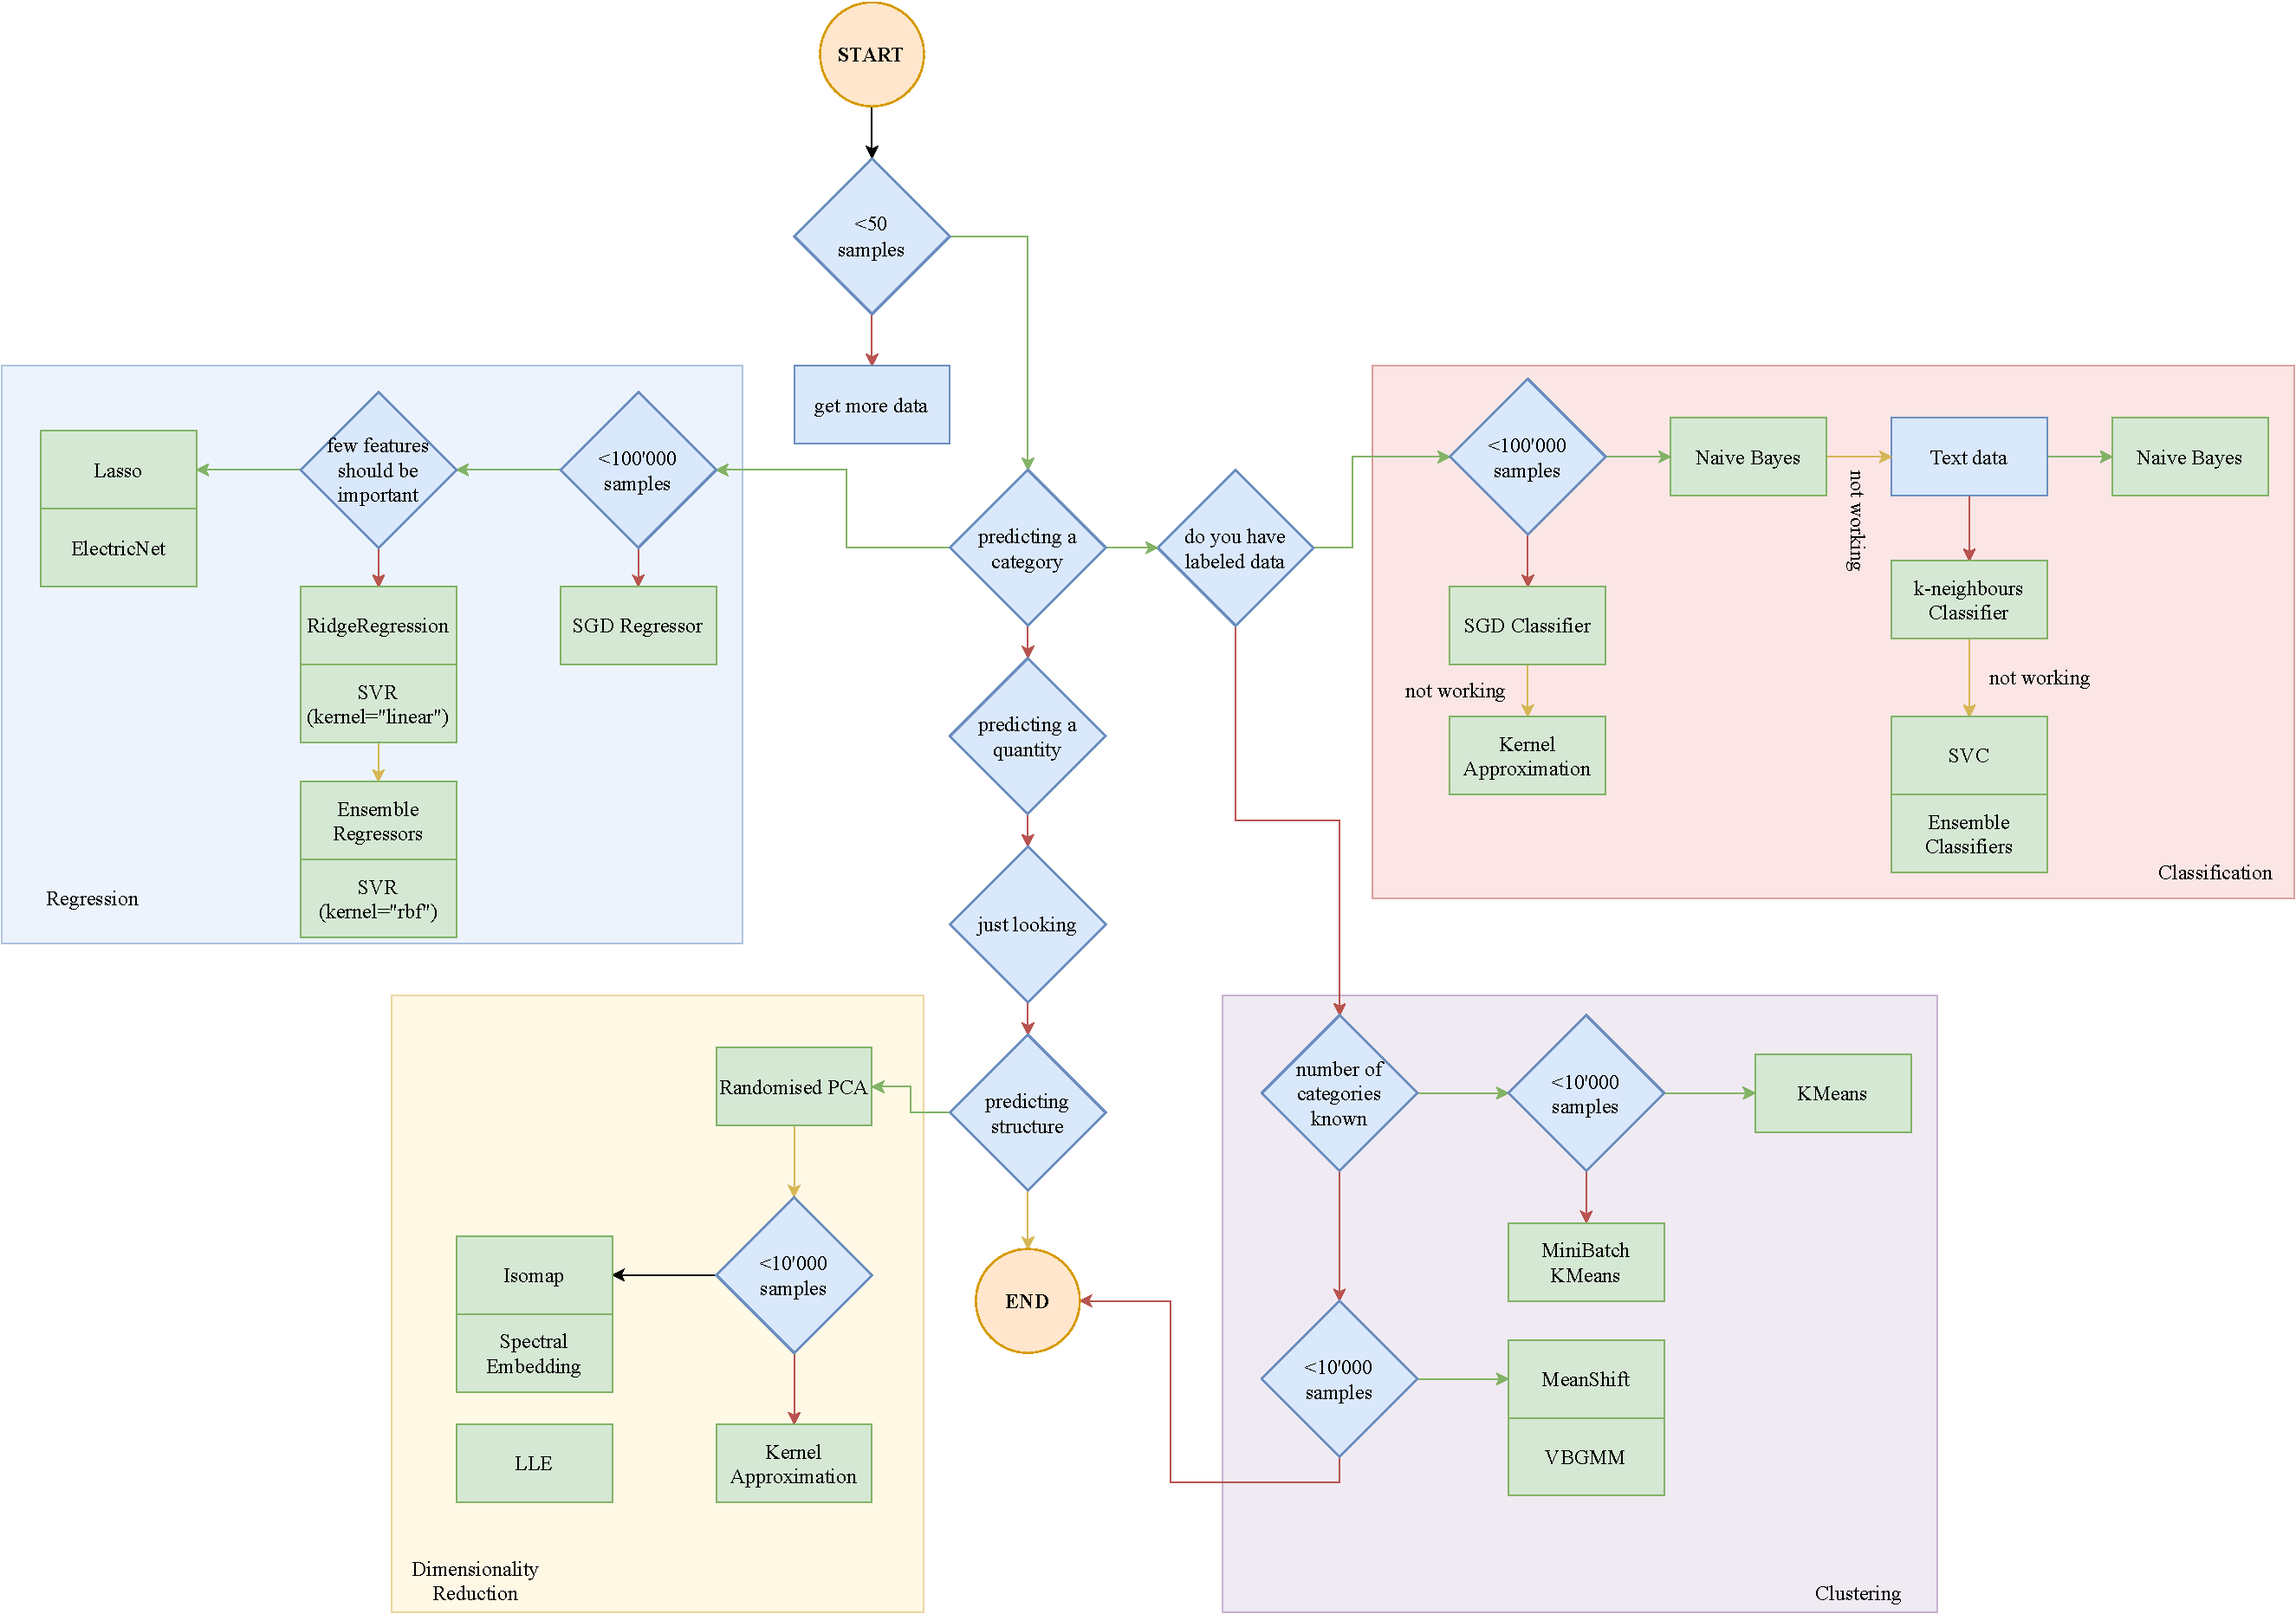
\includegraphics[height=0.9\textheight, keepaspectratio]{scikit-learn_algorithm_cheatsheet}
	\end{center}
\end{landscape}

\subsection{Inductive Supervised Learning}
The data usually has a semi-formal representation in attribute-label pairs $(\textbf{x}, y)$. The labels encode concepts or classes.
Approximate the mapping function from example $x$ to label $y$ with a hypothesis $h(x) = \hat{y} \approx f(x)$ so that it generalises well.

\subsection{Learning as Search}
\begin{center}
	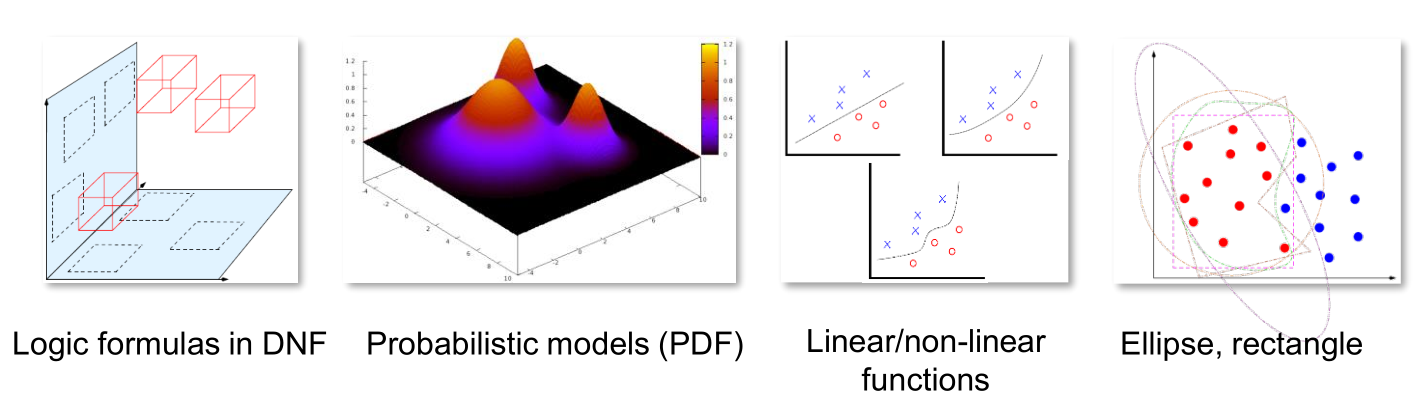
\includegraphics[width=0.7\linewidth]{img/hypothesis_space}
\end{center}

The hypothesis space $\Hilbert$ contains all possible hypotheses that can be built with the chosen representation, learning can thus be understood as a search for the global minima in this space \Hilbert.

\noindent
Formally this goal is expressed as follows: Find the hypothesis $h^* (x,\theta) = \hat{y}$ that best fits the training data, according to a loss or cost function $L(h(x,\theta))$ by searching the hypothesis space $\Hilbert = \left\{ h(x,\theta) \middle| \theta \in P\right\}$.

\subsection{Inductive Bias}
\begin{theorem}
	A learner that makes \textbf{no a-priori assumptions} regarding the identity of the target concept has \textbf{no rational basis for classifying} any unseen instances. - Mitchell
\end{theorem}
All learning algorithms have some preformed hypothesis that is helpful to look for. It is beneficial to choose algorithms whose implicit hypothesis fits the data.

No free lunch theorem regarding the general equivalence of learners states that if all functions $f$ are equally likely, the probability of observing an arbitrary sequence of cost values during training does not depend on the learning algorithm $\mathcal{L}$.

The inductive bias of a learning algorithm $\mathcal{L}$ for instances in $X$ are any \textbf{minimal set of assertions} $B$ that, together with $\mathcal{L}$ and the training set $D$ \textbf{allows for deductively inferring} the $y'$ for a new $x\in X$. Make all assumptions \textbf{explicit} in $B$ such that $\forall x' \in X: \left(B, \mathcal{L}, D, x' \right) \Rightarrow y'$ is provable.

Machine Learning depends on the intelligent choice of the class \Hilbert where $\mathcal{L}$ optimises the parameters. Machine Learning algorithms can be categorised by the strength of their inductive bias.

\subsection{Inductive Unsupervised Learning}
\begin{minipage}{0.6\linewidth}
	The usual task is Clustering, where the data $D$ are described by feature vectors without any labels, interesting structures and relationships in the data are then searched. The data naturally fall into $K$ groups, where the number of classes are not determined at the start but found through the learning scheme. This presents the challenge of searching by similarity in \textbf{distance} or \textbf{density}, which is another inductive bias to be considered, and by the choice of \textbf{parameters}.
	
\end{minipage}
\begin{minipage}{0.4\linewidth}
	\begin{center}
		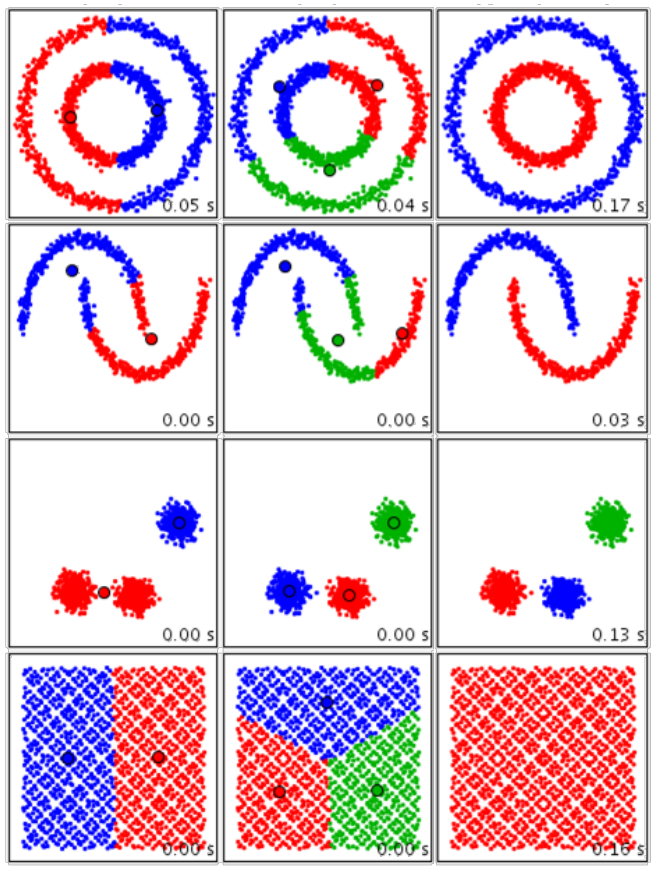
\includegraphics[width=0.6\linewidth]{img/clustering_example}
	\end{center}
\end{minipage}

\subsection{Learnability}
Any target function $f$ over an instance $X$ is learnable given an expressive enough deterministic hypothesis space \Hilbert, a large enough training set $D$, and stationarity of the distribution $X$, that is instances in $D_{\text{train}}$ and $D_{\text{test}}$ are independently, identically distributed.

Better questions are what size of \textbf{$D_{\text{train}}$} are large enough and given a large enough training set, how well does the \textbf{training error predict generalisability}. These questions are in the domain of \emph{computational learning theory}.

\subsection{Probably Approximate Correct Learning and Vapnik-Chervonenkis Complexity}
Sample complexity bounds using $\abs{\Hilbert}$ usually do substantially overestimate, thus the assumption that $\bm{f} \in \Hilbert$ is unrealistic.

Measuring Vapnik-Chervonenkis (VC) dimension for infinite \Hilbert:
$h\in\Hilbert$ is \textbf{shattering a set of instances} $S\in X$ \textbf{iif} $h$ can partition $S$ in any way possible.\\
$VC(\Hilbert) := \abs{\{S\in X | S\ \text{is the largest subset of}\ X\ \text{shattered by any}\ h\in\Hilbert\}}$. $VC(\Hilbert)$ can be used as an alternative measure of $\abs{\Hilbert}$ to compute sample complexity.

\begin{figure}[H]
	\centering
	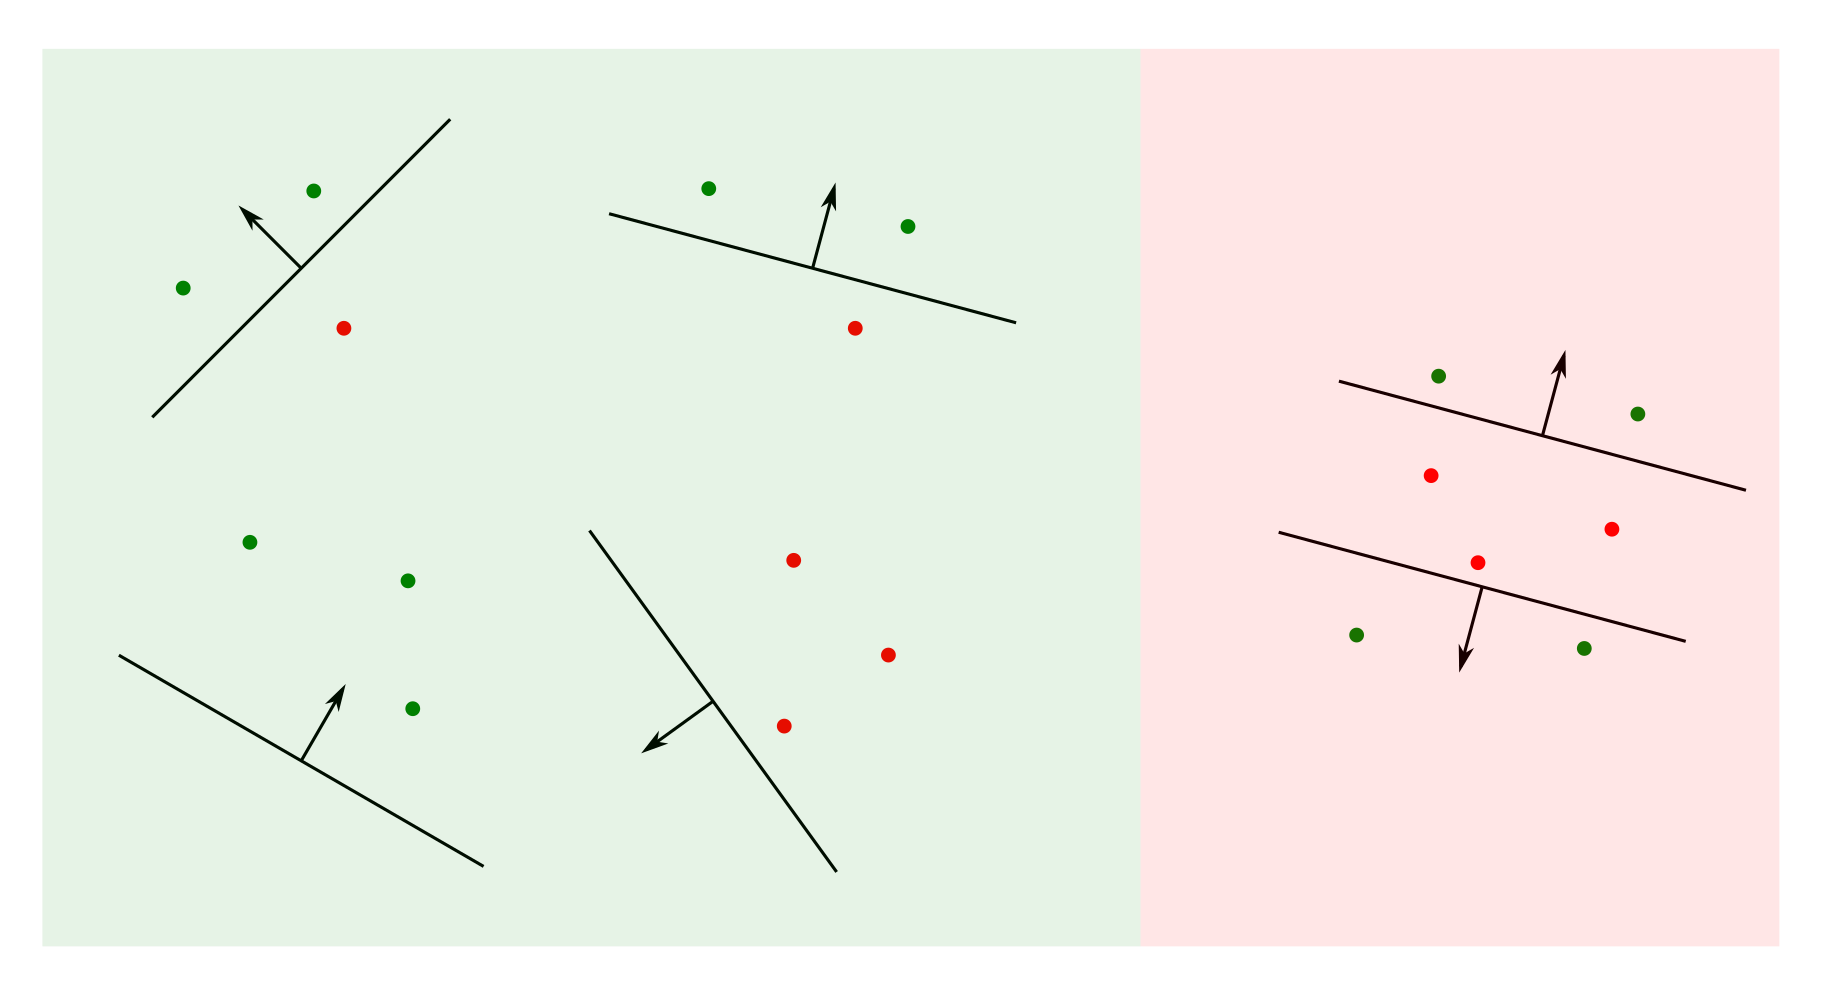
\includegraphics[keepaspectratio,width=0.9\linewidth]{VC_shattering}
	\caption{A two-dimensional linear classifier can shatter three points, $VC(\text{two-dimensional straight lines}=3$ but $\abs{\Hilbert} = \infty$}
\end{figure}

\section{Formulating Learning Problems}
\subsection{Designing a Learning Solution}
\begin{center}
	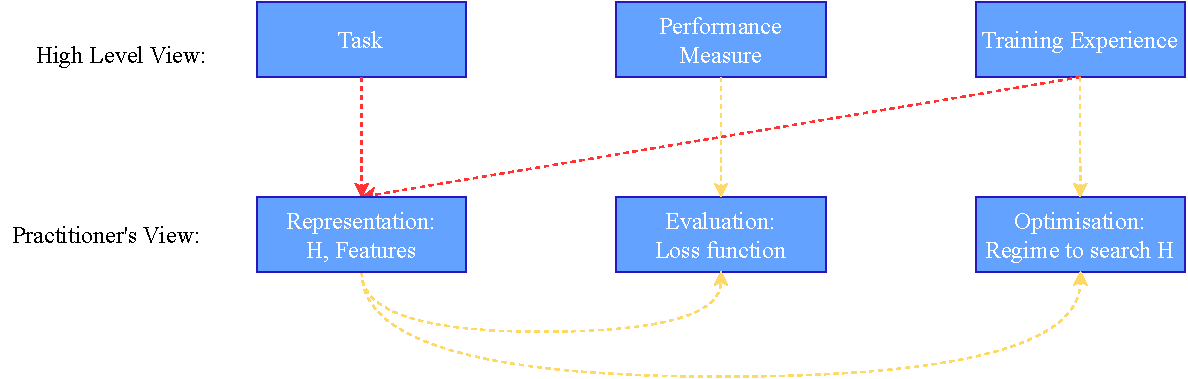
\includegraphics[width=\linewidth,keepaspectratio]{designing_learning_solution.pdf}
\end{center}

Designing a problem that is easiest for the algorithm to solve is the best thing one could do while formulating the problem. The first thing to do while first analysing data is to plot it.

\subsection{Machine Learning Development Process - Exploration and Experimentation}
There is a necessity to have a distinct conceptual approach to model data. Focus on \textbf{systematic experimentation} and \textbf{rigorous evaluation}, even automatised if needed. This is best implemented by a \textbf{pipeline of scripts} similar to the UNIX command line approach. Data exploration and rapid prototyping is key in the beginning of this process.

\begin{center}
	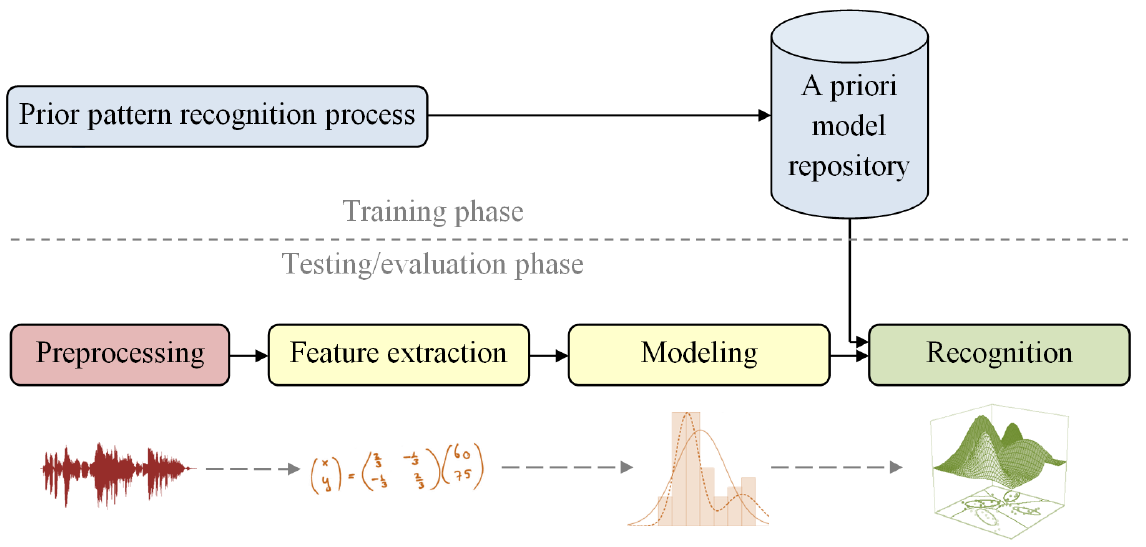
\includegraphics[width=0.6\linewidth]{exploration_evaluation_pipeline}
\end{center}

\section{Machine Learning Guiding Principles}

\subsection{Cost Function J}
Choose $\theta_0, \theta_1$ in such a way that $h(x)$ is close to $y$ for the training examples $(x,y)$. Let a function $J$ \textbf{number the cost of errors made} for the specific set of parameters.

\begin{equation*}
	J_{MSE}(\theta_0, \theta_1) = \frac{1}{2N} \sum_{i=1}^{N} \left(h(x_i, \vec{\theta}) - y_i\right)^2
\end{equation*}

The objective is to minimise $J$ with regards to $\theta_0, \theta_1$

\subsection{Optimisation by Gradient Descent}
Algorithm
\begin{itemize}
	\item Start with a random $\theta_0, \theta_1$
	\item Keep changing $\theta_0, \theta_1$ in a way to reduce $J(\theta_0, \theta_1)$
	\item End at a local minimum
\end{itemize}

\begin{align*}
	\text{\texttt{tmp\_0}} &:= \theta_0 - \alpha \cdot \frac{\partial J}{\partial \theta_0} J(\theta_0,\theta_1)\\
	\text{\texttt{tmp\_1}} &:= \theta_1 - \alpha \cdot \frac{\partial J}{\partial \theta_1} J(\theta_0,\theta_1)\\
	\theta_0 &:= \text{\texttt{tmp\_0}}\\
	\theta_1 &:= \text{\texttt{tmp\_1}}\\
\end{align*}

$\alpha$ is called the learning rate, and is a data-dependent hyper-parameter of the algorithm.

\section{Model Assessment and Selection}

\subsection{Data Handling for Model Evaluation}
Search for methods that help to learn and evaluate algorithms based on \emph{limited data} and help to \emph{deduce the true error} from the training error.

\begin{itemize}[leftmargin=*, labelindent=3cm, labelsep=1cm]
	\item[Model Assessment] \textbf{Evaluate} a model's \textbf{performance}
	\item[Model Selection] \textbf{Select} among competing models the one with the \textbf{proper level of flexibility}
\end{itemize}

\begin{center}
	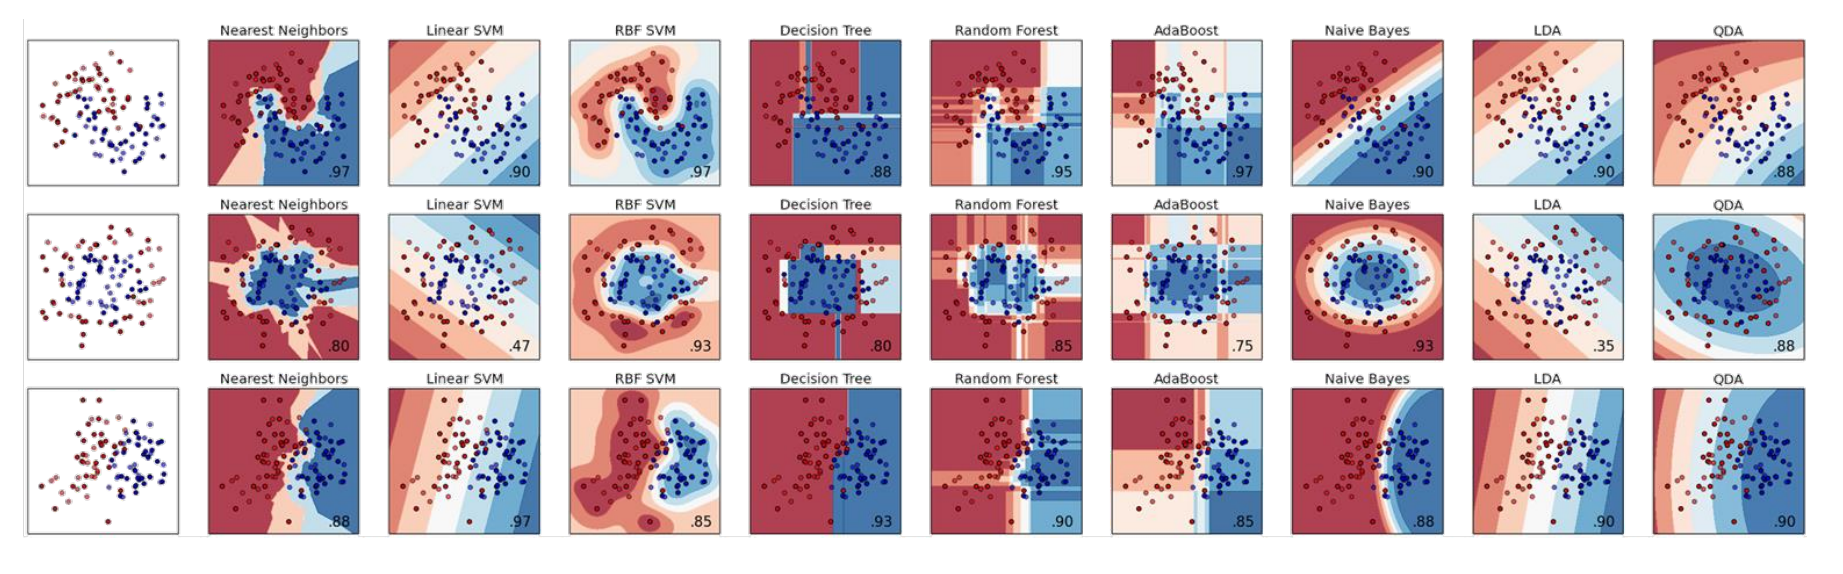
\includegraphics[width=0.9\linewidth]{img/model_flexibility}
\end{center}

\subsection{Optimal Usage of a Small Dataset}
Split into Training, Validation and Test set. Do k-fold Cross Validation on Training and Validation set, final test on Test set. Train k times on $(l - 1)$ folds, validate on the remaining one (until each fold was used for validation once), then average the error.

\subsection{Observable and Unobservable Errors}
True error $E_D$ is the probability that $h$ will misclassify a random instance from the \textbf{complete domain} $\bm{E}$ and is unobservable.

The empirical test error $E_{emp}$ is the proportion of \textbf{sample $S\in D$} misclassified by $h$ is en estimate for the true error and gets better with more error.

\begin{itemize}
	\item Assumption that training and test data are representative of underlying distribution of $D$
	\item $S$ and $h$ are usually not chosen independently, that means that the test error is \textbf{optimistically biased}
	\item The test error usually varies for different $S\in D$, that means it has a higher variance than the true error
\end{itemize}

\subsection{Error Sources}

The chosen hypothesis \Hilbert is the \textbf{best hypothesis at a distance of the true function}. Different chosen samples $X$ give \textbf{different information}.

\noindent
Error decomposition:
\begin{equation*}
	E_{MSE} = \underbrace{\text{systematic error}}_{\text{bias}} + \underbrace{\text{dependence on specific sample}}_{\text{variance}}  + \underbrace{\text{random nature of process}}_{\text{irreducible noise or Bayes rate}}
\end{equation*}

\subsection{ROC Curve}
First used in signal detection to show trade-off between \textbf{hit rate} and \textbf{false alarm rate} over noisy channel

\begin{center}
	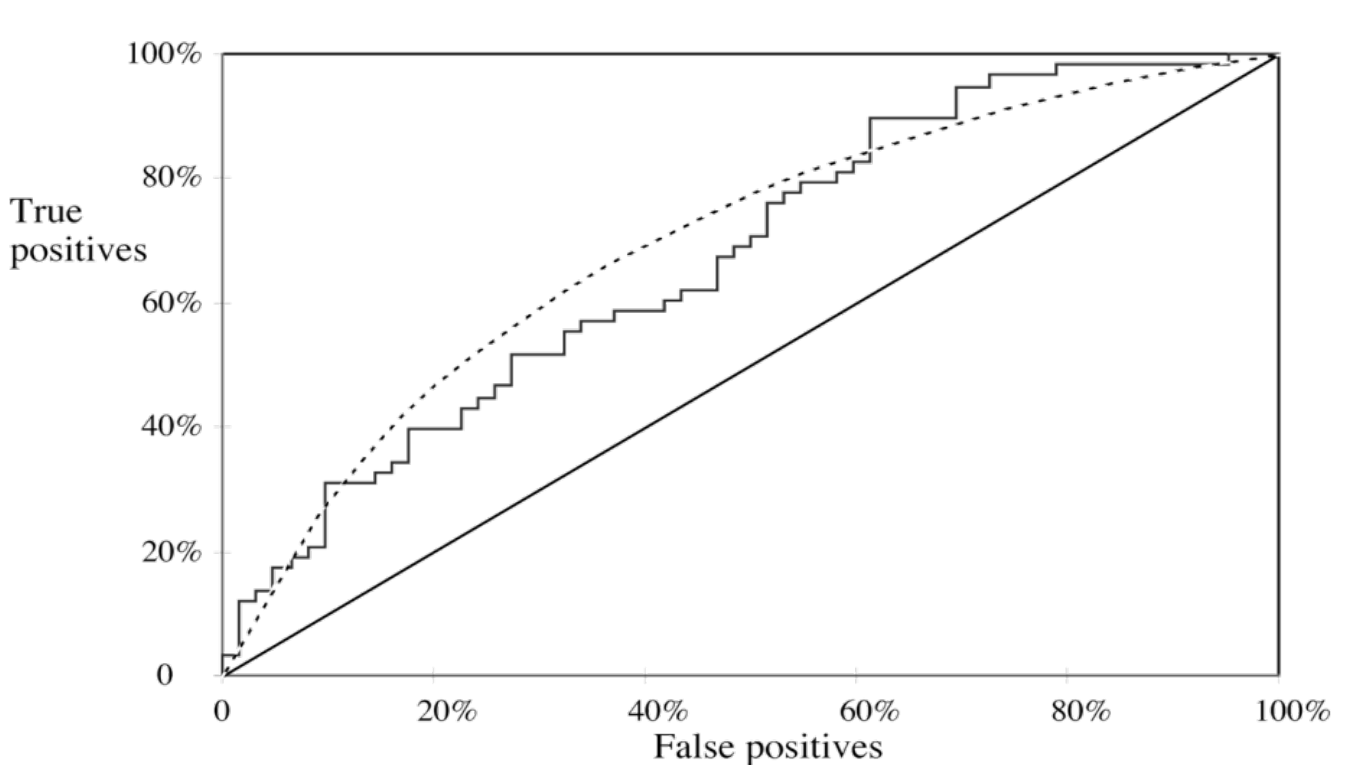
\includegraphics[width=0.7\linewidth]{img/ROC_curve}
\end{center}

\noindent
\textbf{Interpretation}
\begin{itemize}[leftmargin=*, labelindent=3cm, labelsep=1cm]
	\item[Straight Line] Indicates a random process
	\item[Jagged Curve] Created with one set of test data
	\item[Smooth Curve] Created using averages
\end{itemize}

\subsection{Error Measures}
\begin{tabularx}{\linewidth}{lX}
	Mean Square Error & $ E_{MSE} = \frac{1}{F}\sum_{i=1}^{N} (\widehat{y}_i - y_i)^2 $\\
	Root Mean-Squared Error & $E_{RMSE} = \sqrt{\frac{1}{F}\sum_{i=1}^{N} (\widehat{y}_i - y_i)^2 } $\\
	Mean Absolute Error & $ E_{MAE} = \frac{1}{F}\sum_{i=1}^{N} \abs{\widehat{y}_i - y_i}$\\
	(less sensitive to outliers)
\end{tabularx}

\subsection{Evaluating Clustering Methods}
\textbf{Without Labels}:\\
Use the \textbf{silhouette coefficient}, which is a measure for cluster validity or consistency, do a visual inspection of dendrograms and a visual comparison of the dimension reduction o the feature vectors.

\vspace{1em}
\noindent
\textbf{With ground truth available}:\\
Check \textbf{purity}, \textbf{rand index} and \textbf{misclassification rate}.

\subsection{Selection Among Competing Models}
On what basis can one \emph{algorithm be favoured over another} and how probable is it that the chosen method is \emph{truly significantly better}.

\subsection{Maximum Likelihood and Ockham's Razor}
Given competing $h_i \in \Hilbert_j$ \textbf{maximum likelihood parameters} can be found by \textbf{calculating the likelihood} $p(X|h_i)$ and \textbf{selecting the best} $\hat{h} = \underset{h_i}{\max} p(X|h_i)$.

The goal is to find a compromise between model complexity and accuracy on the validation data. Ockham's razor, an axiom in machine learning, states that "given two models with the \textbf{same empirical error}, the simpler one should be preferred because \textbf{simplicity is desirable in itself}". The reasoning is that for a simple hypothesis the \textbf{probability of it having unnecessary conditions is reduced}.

\subsection{Determining True Best Classifier}
In practice tenfold cross validation is often good enough and it does not matter which classifier is really better. Otherwise the \textbf{Student's t-test} can be used to compare two samples. Generally, the difference between $\mu_{\mathcal{L}_A}$ and $\mu_{\mathcal{L}_A}$ of the obtained cross-validation error estimates follows a Student's distribution with $m-1$ degrees of freedom.

If the number of features $p$ is large in comparison to the number of instances $N$ use \textbf{boosting} or \textbf{SVM}. If the data set is \emph{severely imbalanced}, \textbf{non-standard loss functions} that take class distribution in account or \textbf{Bayesian methods} and appropriate prior probabilities should be considered.

\section{Support Vector Machines}

Each observation is a vector of values ($p$-dimensional) for which the SVM \textbf{constructs a hyperplane} to separate class members. There are different support vectors for different tasks
\begin{enumerate}
	\item Maximal margin \textbf{hyperplane} classifier, for linearly separable data
	\item Support vector \textbf{classifier}, for almost linearly separable data
	\item Support vector \textbf{machine}, for non-linearly separable data
\end{enumerate}

\subsection{Maximal Margin Classifier}
\begin{minipage}{0.6\linewidth}
	Chooses the hyperplane maximising the distance from the hyperplane to the closest training point, denoted the support vectors, and can be represented as a linear combination of only a few training points.
\end{minipage}
\begin{minipage}{0.4\linewidth}
	\centering
	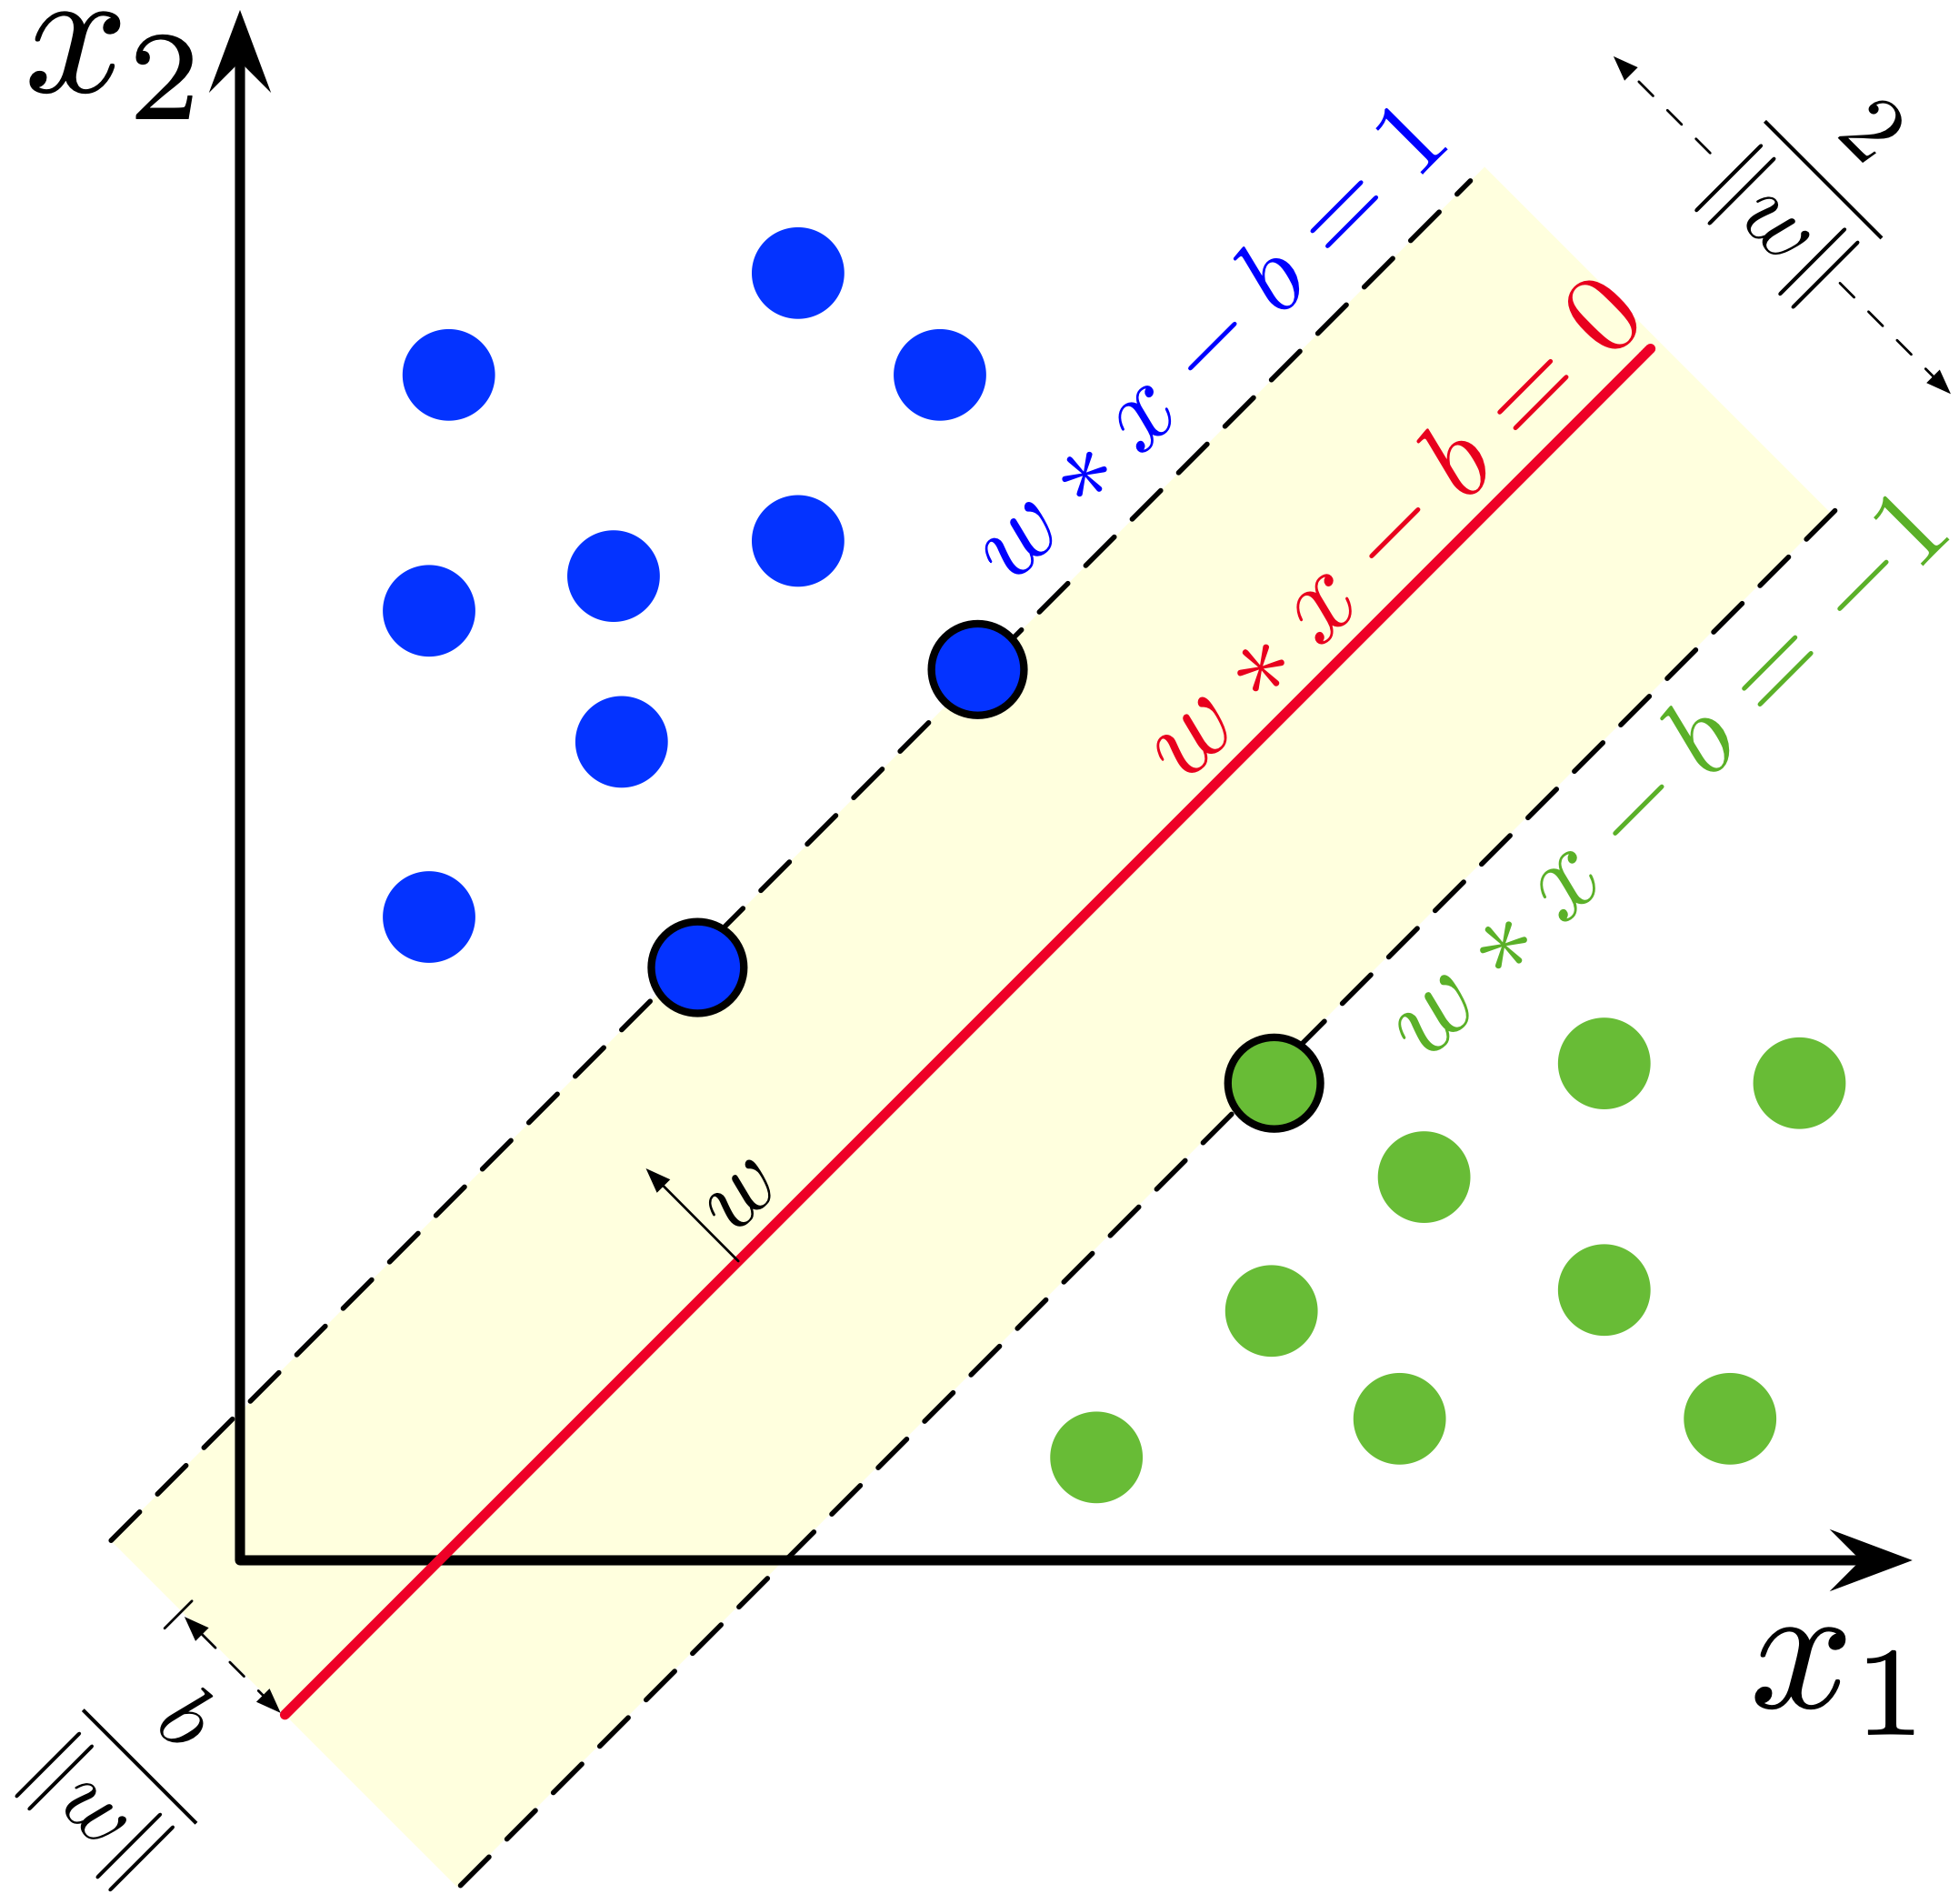
\includegraphics[keepaspectratio,width=0.8\linewidth]{img/maximum_margin_classifier.png}
\end{minipage}

\begin{definition}
	Definition of a hyperplane
	\begin{equation*}
		\{ \vec{x}: \beta_0 + \beta_1 x_1 + \beta_2 x_2 + \dots + \beta_p x_p = 0 \}
	\end{equation*}
\end{definition}
Separating hyperrplanes for classes encoded $\pm 1$
\begin{align*}
	\beta_0 + \beta_1 x_{i1} + \beta_2 x_{i2} + \dots + \beta_p x_{ip} &> 0 \qquad \text{if}\ y_i = 1\\
	\beta_0 + \beta_1 x_{i1} + \beta_2 x_{i2} + \dots + \beta_p x_{ip} &< 0 \qquad \text{if}\ y_i = -1\\
	\intertext{Equivalently}
	y_i\cdot (\beta_0 + \beta_1 x_{i1} + \beta_2 x_{i2} + \dots + \beta_p x_{ip}) &> 0
\end{align*}
Evaluating the hyperplane formula for a point $x$ gives its distance to the hyperplane, if $\bm{\beta}$ is a normal vector.

\subsection{Formulation of Optimisation Problem}
Intuitive Optimisation
\begin{itemize}[noitemsep]
	\item $\underset{\beta_0,\beta_1,\dots,\beta_p}{\text{maximise}} M$
	\begin{itemize}
		\item subject to $\sum_{j=1}^{p}\beta_j^2 = 1$
		\item and $y_i\cdot (\beta_0 + \beta_1 x_{i1} + \beta_2 x_{i2} + \dots + \beta_p x_{ip}) \geq M\qquad\forall i = 1..N$
	\end{itemize}
\end{itemize}
This can be reformulated using {\color{DodgerBlue2} Lagrange multipliers}
\begin{itemize}[noitemsep]
	\item Find $L_D = \sum_{i=1}^{N} \alpha_i - \frac{1}{2} \sum_{i=1}^{N}\left( \sum_{k=1}^{N} \alpha_i \alpha_k \bm{x}_i^T \bm{x}_k \right) $
		\begin{itemize}
		\item subject to $ \alpha_i \geq 0 $ and $\sum_{i=1}^{N} \alpha_i y_i = 0$
		\item Once the alphas are computed $\beta = \sum_{i=1}^{N} \alpha_i y_i \bm{x}_i$
	\end{itemize}
\end{itemize}

\subsection{Support Vector Classifier}
Based on the assumption that the data is not perfectly linearly separable any more, the idea is to introduce soft margins that allow for \emph{some} misclassifications. The number of misclassifications is controlled by a {\color{DodgerBlue2} penalty factor} $C$.

\begin{center}
	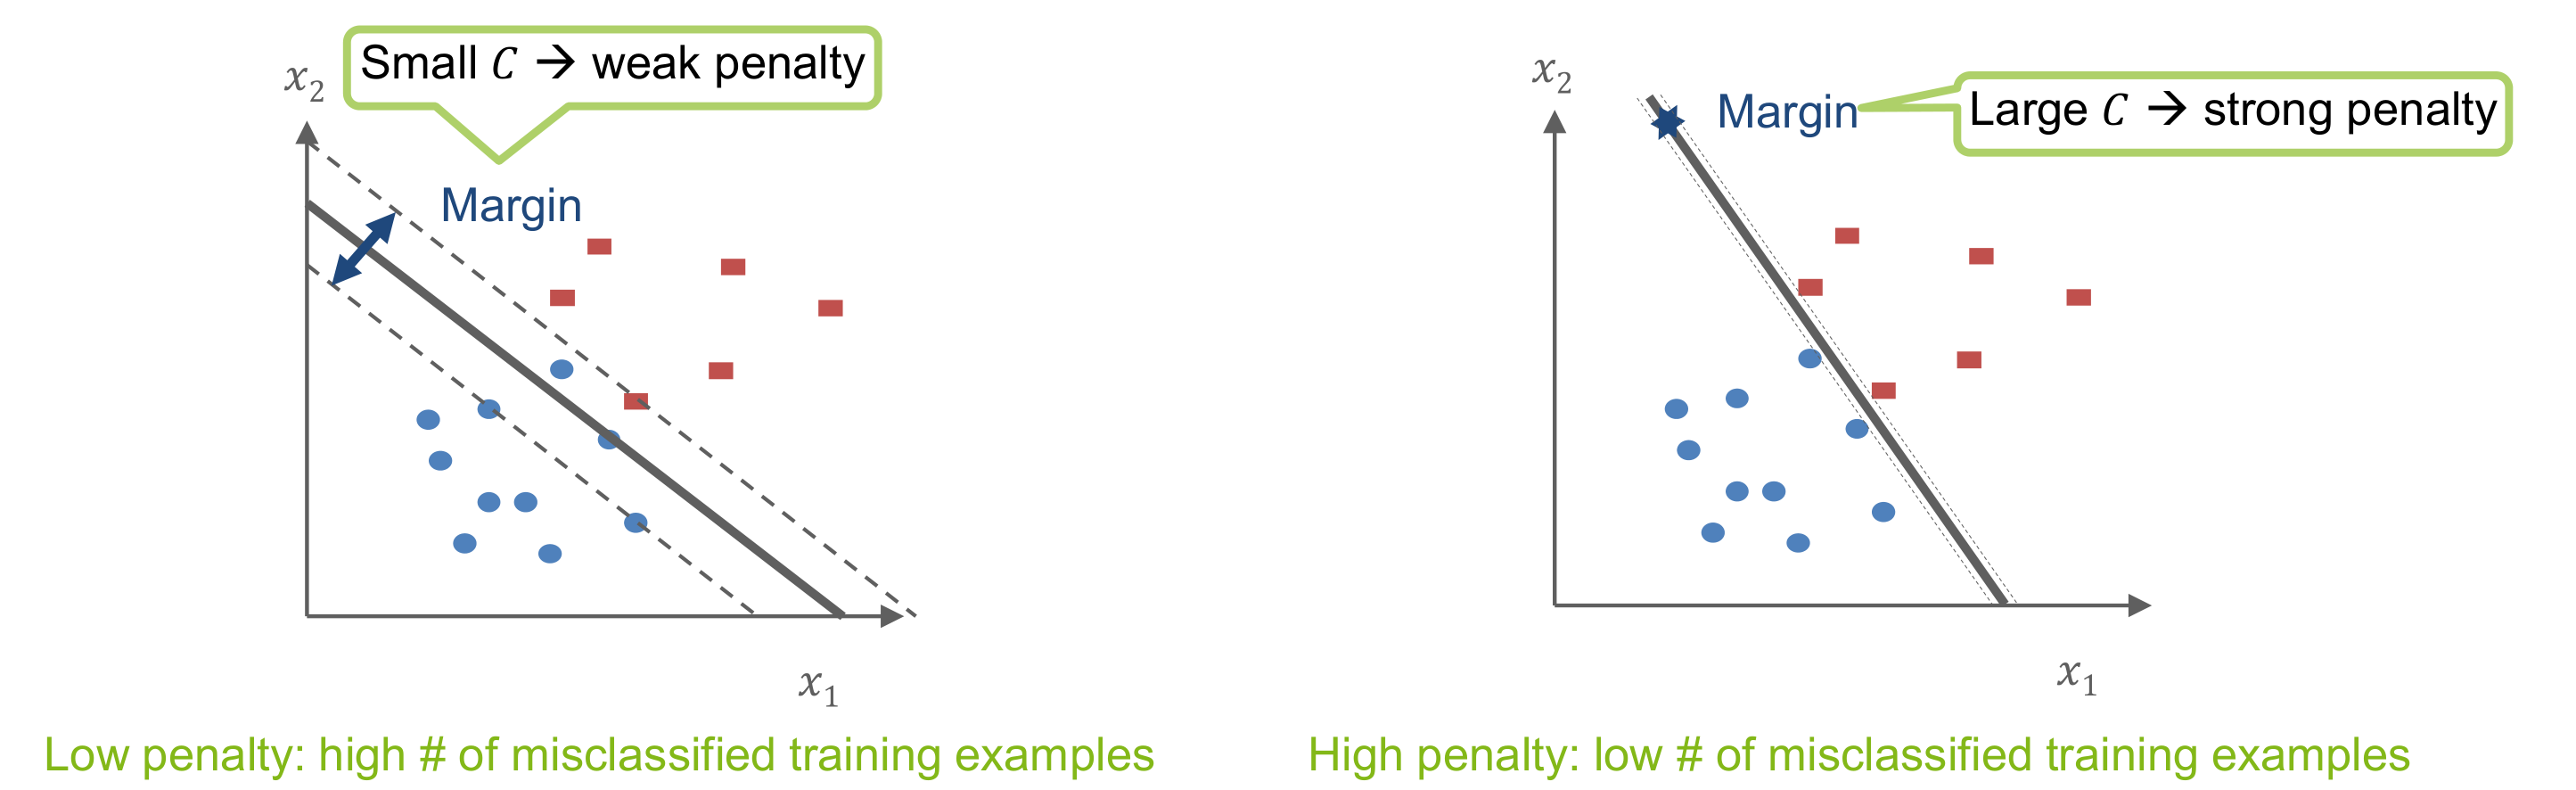
\includegraphics[width=0.7\linewidth]{img/support_vector_classifier}
\end{center}

\subsubsection{Support Vector Classifier Optimisation}
\begin{minipage}{0.6\linewidth}
Intuitive Optimisation
\begin{itemize}[noitemsep,nosep]
	\item $\underset{\beta_0,\beta_1,\dots,\beta_p}{\text{maximise}} M$
	\begin{itemize}
		\item subject to $\sum_{j=1}^{p}\beta_j^2 = 1$
		\item and $y_i\cdot (\beta_0 + \beta_1 x_{i1} + \beta_2 x_{i2} + \dots + \beta_p x_{ip}) \geq M(1 - \xi_i)   \qquad\forall i = 1..N$
		\item $\xi_i \geq 0, \sum_{i=1}^{N}\xi_i \leq \tilde{C}$
		\item where $\xi_i$ is a slack variable to allow instance $i$ to lie on the wrong side of the margin
		\item $\tilde{C}$ is the total budget for misclassifications
	\end{itemize}
\end{itemize}
Equivalent technical optimisation, so called "dual form"
\begin{itemize}[noitemsep,nosep]
	\item maximise\\
	$L_D = \sum_{i=1}^{N} \alpha_i - \frac{1}{2} \sum_{i=1}^{N}\sum_{k=1}^{N} \alpha_i \alpha_k y_i y_k x_i^T x_k$
	\begin{itemize}
		\item subject to $0 \leq \alpha_i \leq C$ and $\sum_{i=1}^{N}\alpha_i y_i = 0$
		\item $\beta = \sum_{i=1}^{N} \alpha_i y_i x_i$ is minimised
	\end{itemize}
\end{itemize}
\end{minipage}
\begin{minipage}[t]{0.4\linewidth}
		\centering
		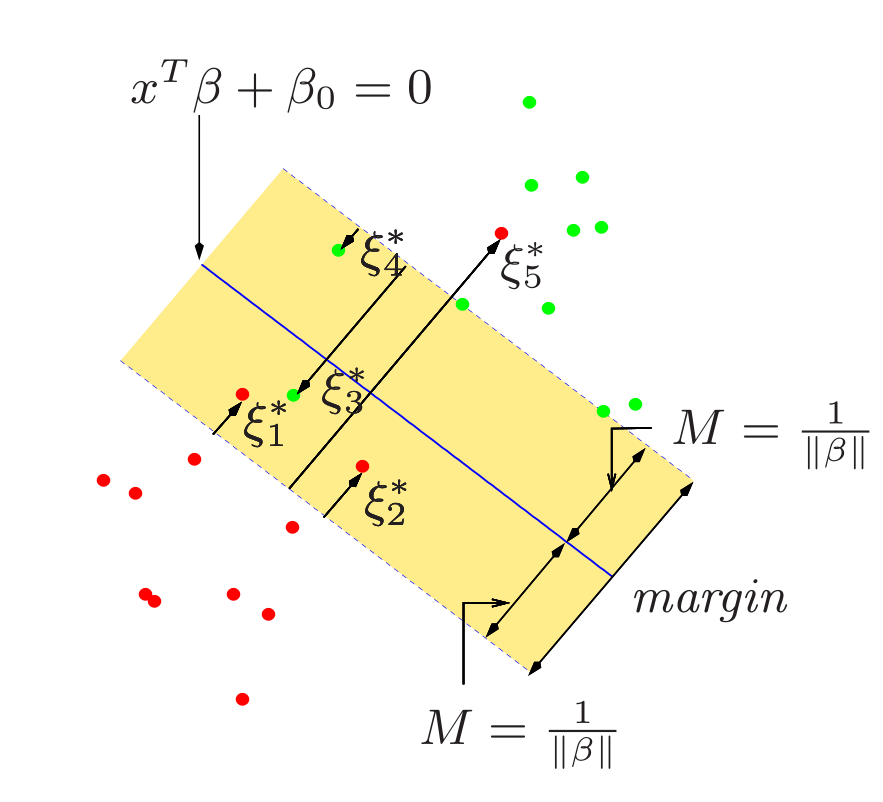
\includegraphics[width=0.8\linewidth]{img/support_vector_classifier_penalty}
\end{minipage}

\subsection{Support Vector Machines}
A possible solution for linearly completely non-separable data is to map the data into a higher-dimensional space. In this space a separating hyperplane may be defined. 

\subsubsection{Variable Transformation}
The same idea applies, transform a non-linearly separable input function in $\R^n$ to $\R^{n+k}, k\geq 1$ where it may be linearly separable.

\begin{center}
	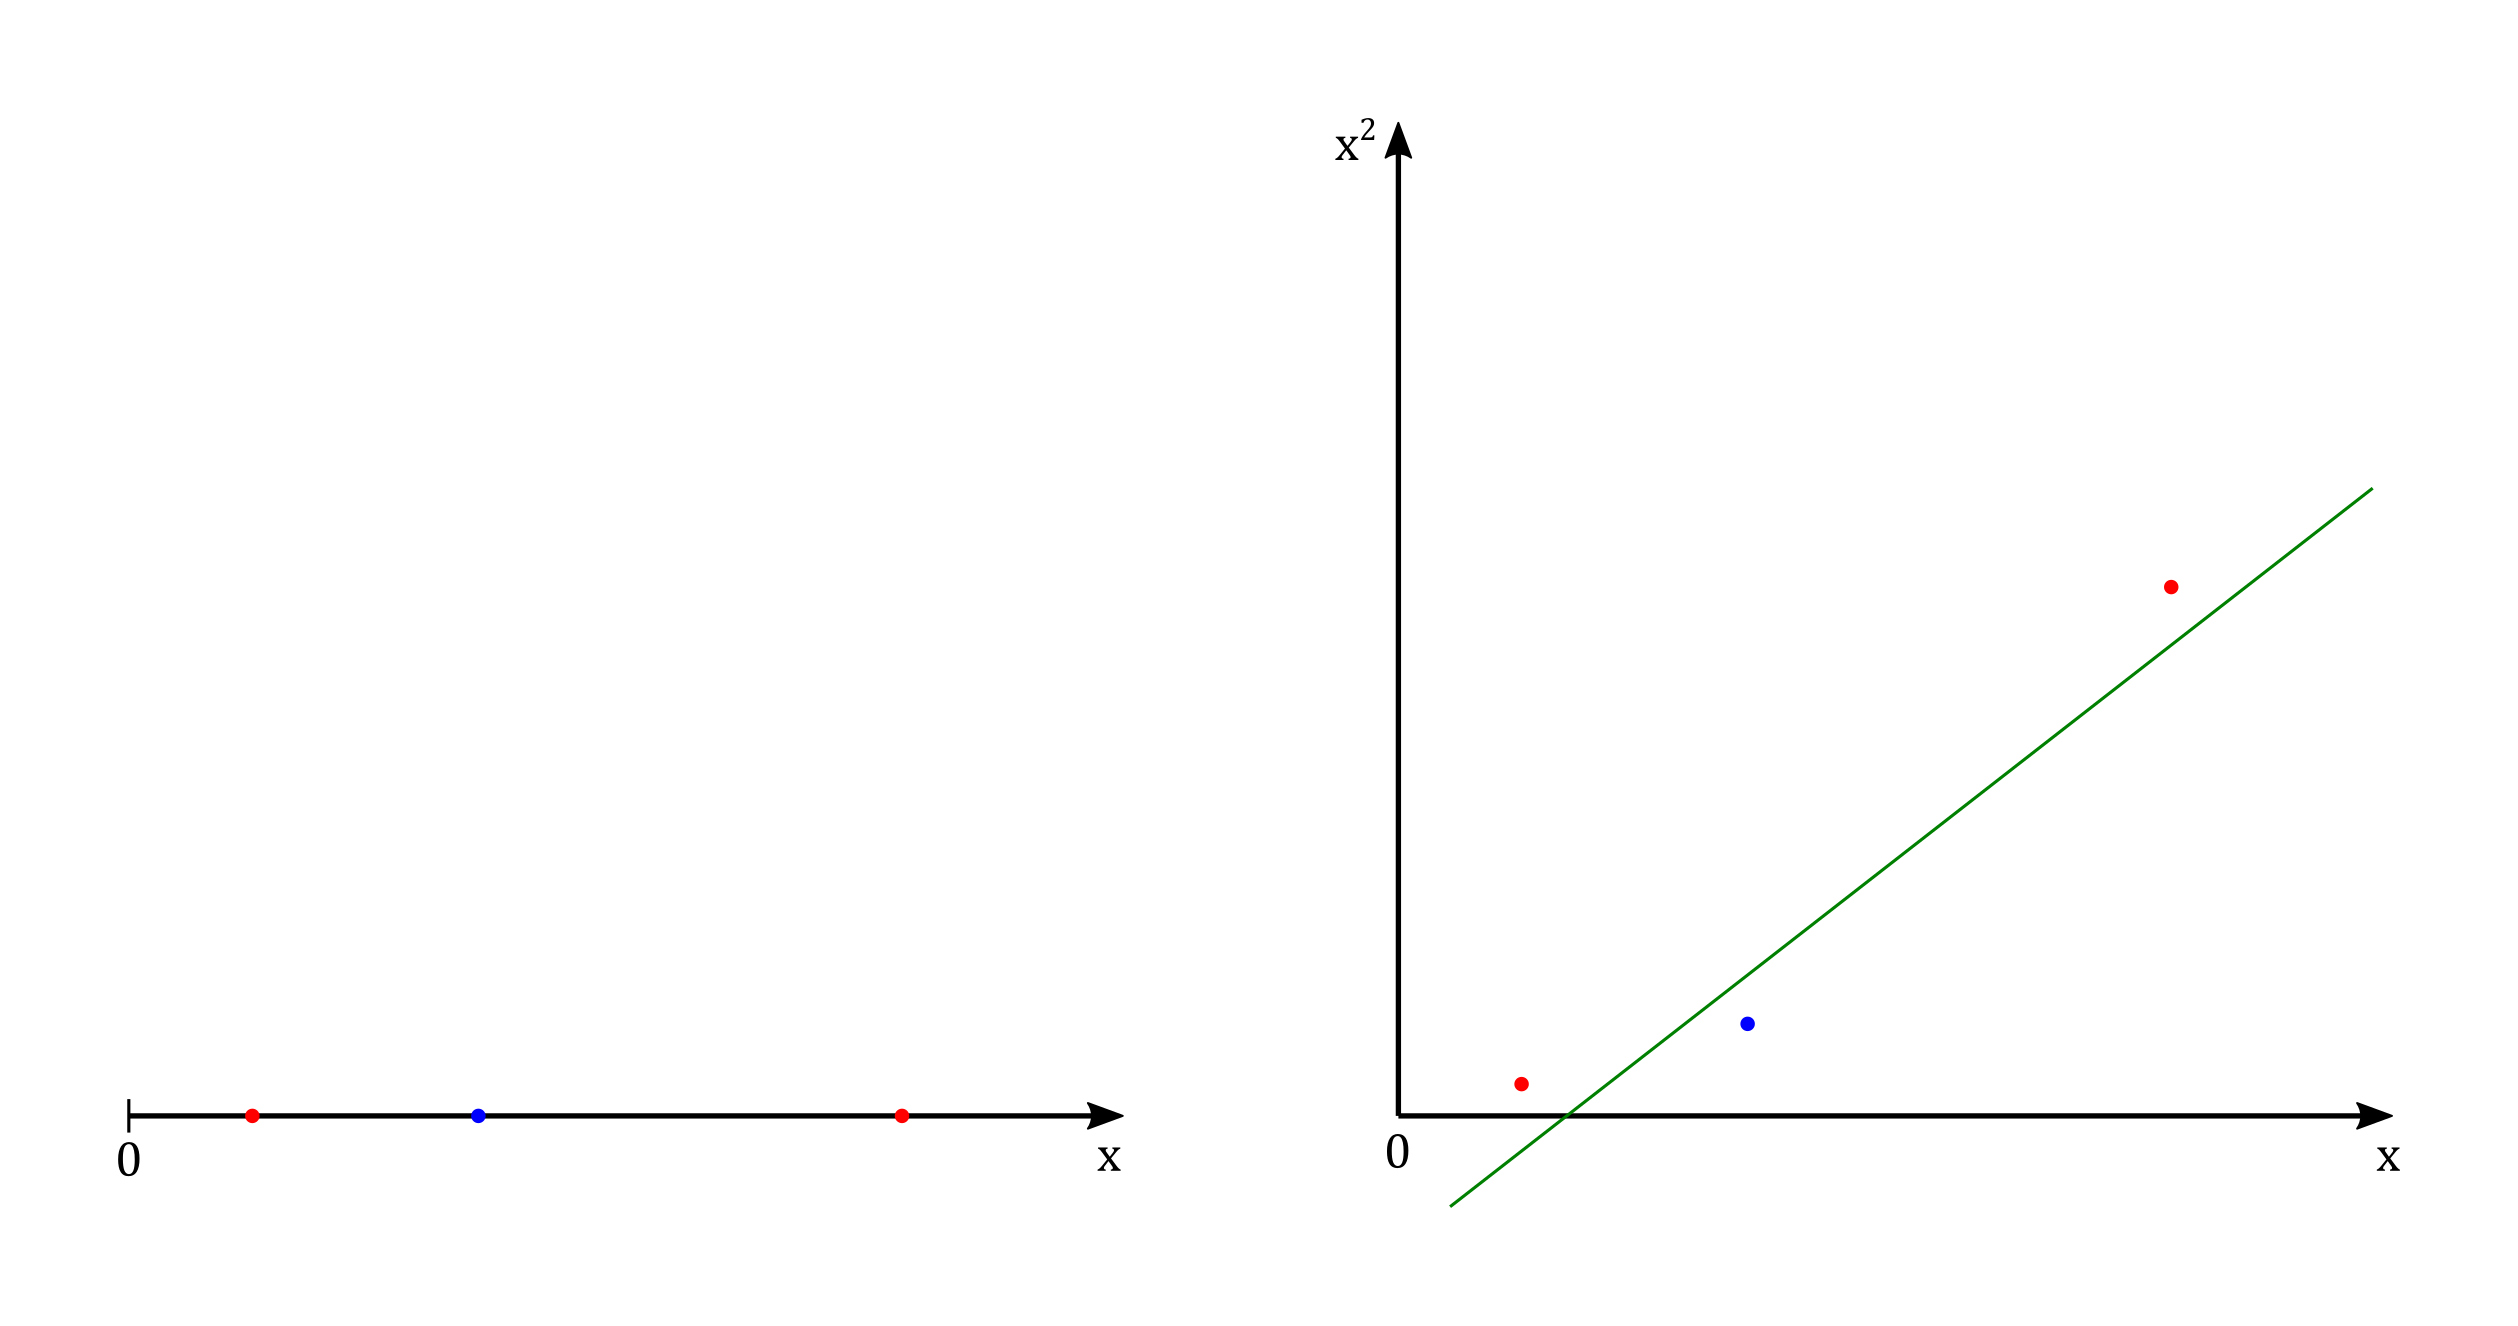
\includegraphics[keepaspectratio,width=0.6\linewidth]{variable_transformation.png}
\end{center}

The power of feature space transformation lies in the fact, that with an appropriately chosen feature space of sufficient dimensionality any consistent training set can be made separable.
\begin{equation*}
	\left\langle \begin{pmatrix}x_i\\x_i^2\end{pmatrix} \cdot\begin{pmatrix}x_{i'}\\x_{i'}^2\end{pmatrix} \right\rangle = x_i x_{i' } + x_i^2 x_{i' }^2 := K(x_i,x_{i'})
\end{equation*}
$K$ is known as a \textbf{kernel} function. It can be used to efficiently compute feature space transformations. Instead of calculating the inner product, the kernel $K(\cdot,\cdot)$ gets calculated. As soon as some $K$ is used, the resulting SVC becomes a SVM.

The following Kernels are common
\begin{itemize}[noitemsep]
	\item {\color{DodgerBlue2} Identity (inner product)}
	\begin{equation*}
		K(x_i,x_{i'}) = \sum_{j=1}^{p} x_{ij}x_{i'j}
	\end{equation*}
	this yields the standard support vector classifier
	\item {\color{DodgerBlue2} Polynomial of degree $d$}
	\begin{equation*}
		K(x_i,x_{i'}) = \left(1 + \sum_{j=1}^{p} x_{ij}x_{i'j}\right)^d
	\end{equation*}
	the polynomial kernel of degree $d = 1$ is just the identity kernel
	\item {\color{DodgerBlue2} Radial basis or Gaussian}
	\begin{equation*}
		K(x_i,x_{i'}) = e^{\left( -\gamma \sum_{j=1}^{p}(x_{ij} - x_{i'j})^2 \right)}
	\end{equation*}
	the Gaussian kernel computes a very local neighbourhood, with $\gamma$ being the hyper-parameter controlling the width of that neighbourhood. A low $\gamma$ yields a great width. The feature space spanned by the Gaussian kernel is implicit and infinite-dimensional.
\end{itemize}

\subsection{Multiclass Classification With Support Vector Machine}
With one versus rest or all classification, the binary classifier SVM can be adapted to choose between multiple classes.
\begin{center}
	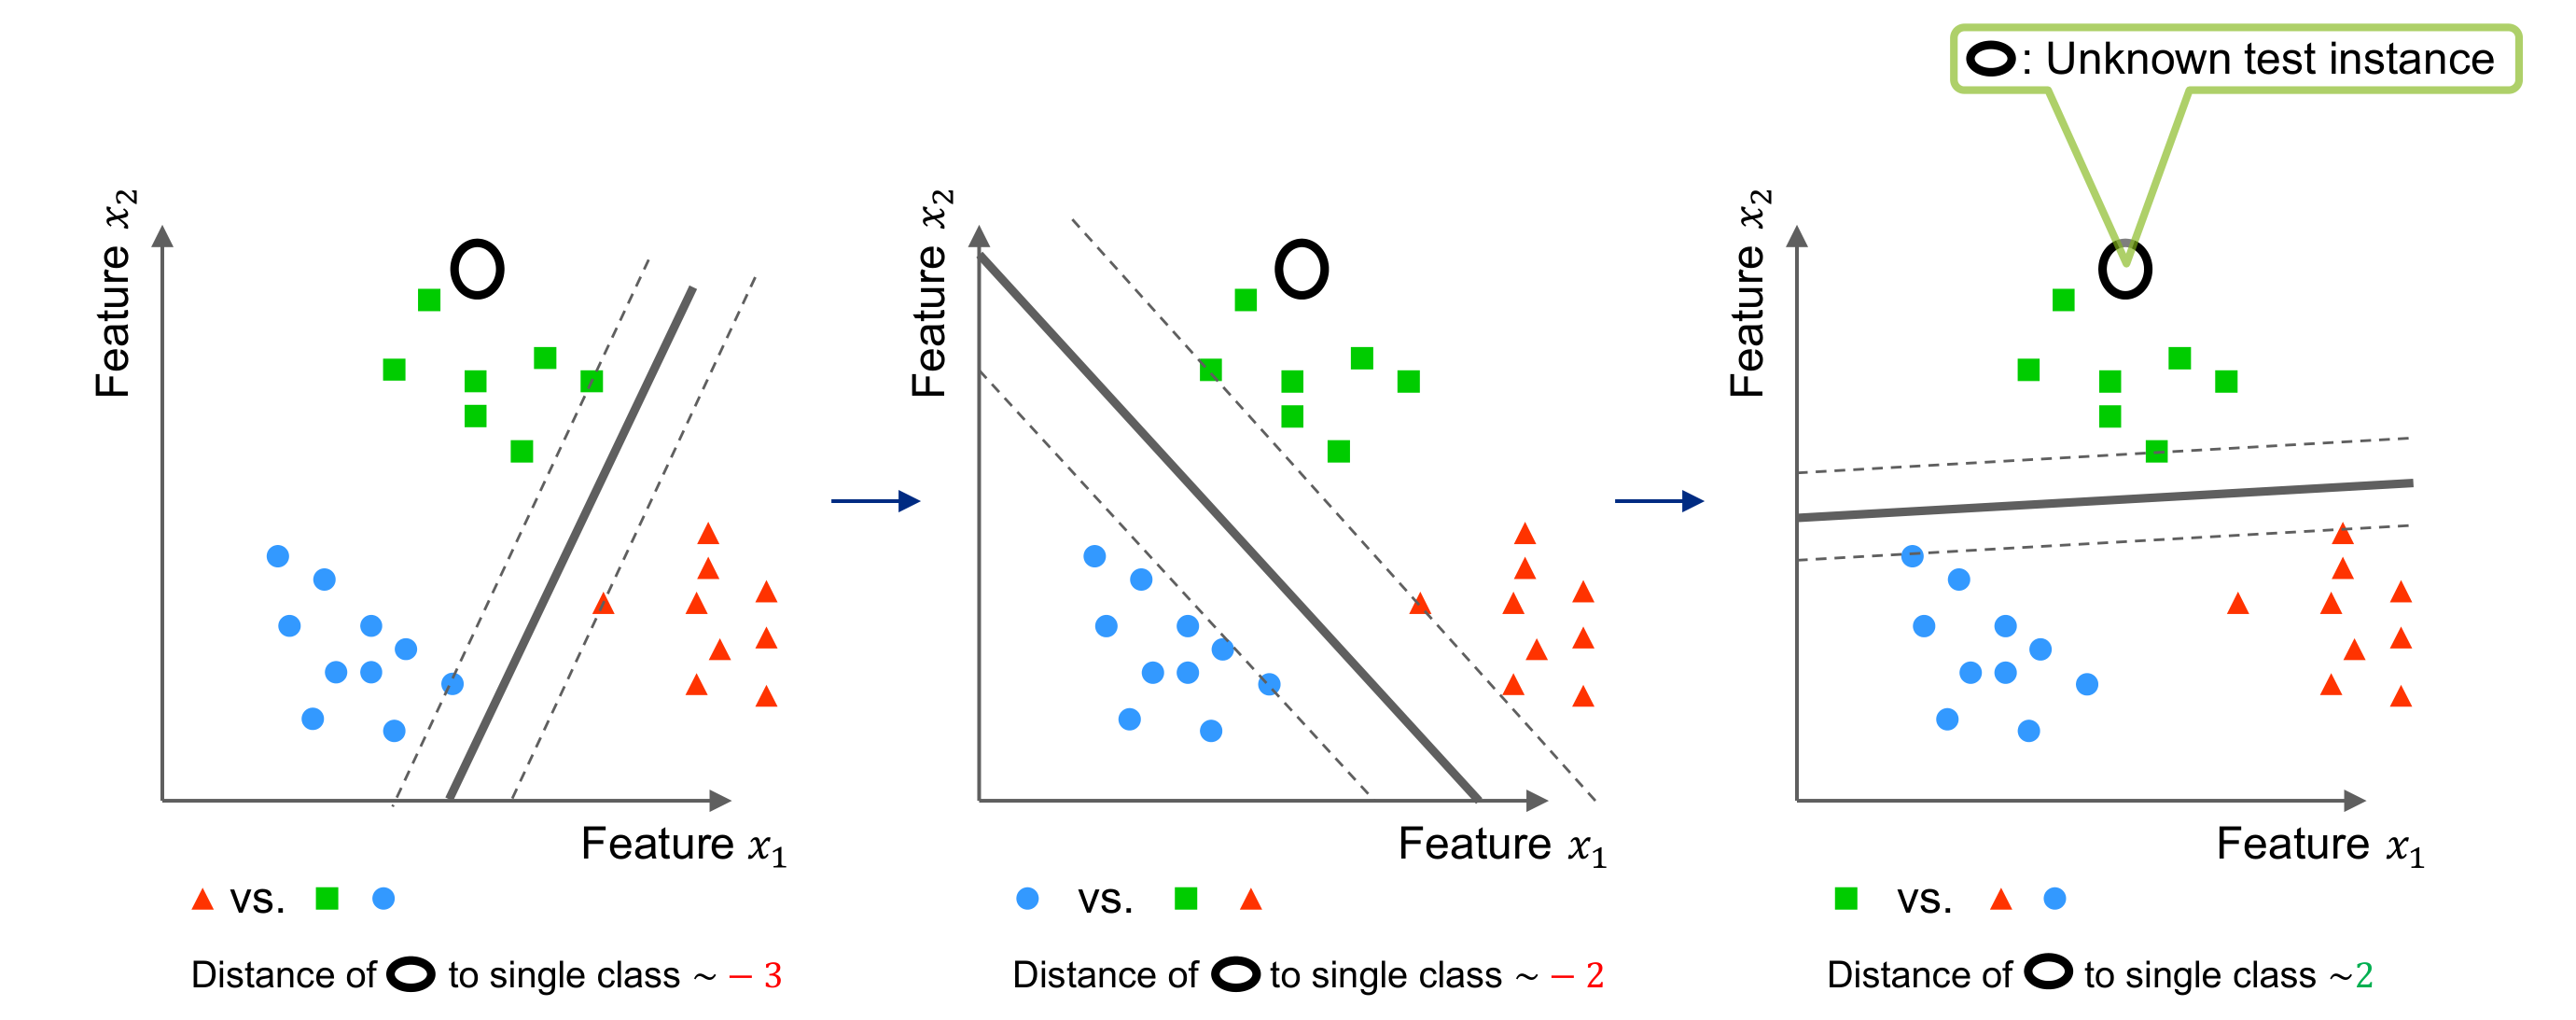
\includegraphics[width=0.8\linewidth]{img/support_vector_machine_multiclass}
\end{center}
Assume $k$ classes, learn all $\frac{k(k-1)}{2}$ pairwise comparisons and classify unknown instances by majority vote among all pairwise comparisons.

\section{Ensemble Methods}
The goal of ensembles is to increase performance by \textbf{combining multiple complementary classifiers}. The intuition behind it is to build different experts and let them decide by vote. This is {\color{Green3} very effective in practice} and has {\color{Green3}good theoretical guarantees}, but while being {\color{Green3} easy to implement} the result {\color{Firebrick3} lacks in transparency}, {\color{Firebrick3}interpretability} and a {\color{Firebrick3} compact representation}.

The formal problem description is: Given $T$ binary classification hypotheses $(h_1,\dots, h_T)$, find a combined classifier with better performance of the form
\begin{equation*}
	\hat{h}(x) = \text{sign}\left( \sum_{t=1}^{T} \alpha_t h_t (x) \right)
\end{equation*}
For regression the average is used.

Ensembles work because they average the error, in statistical terms the bias remains equal but the variance is reduced.

\subsection{AdaBoost}
\subsubsection{Boosting}
The general idea is to boost the performance of weak learners iteratively by making misclassified examples more important and then combining hypotheses. This way, each stage additively corrects shortcomings of previous stages by reweighing and majority voting on the result. The \textbf{Ada}ptive \textbf{Boost}ing algorithm works by
\begin{minted}[escapeinside=||,mathescape=true,fontsize=\small]{python}
initialize weights: |$w_i := \frac{1}{N}$|
for |$ t:=1..T $|
	|$ h_t $| := train decision stump on the |$ x_i $|, weighted by the |$ w_i $|
	|$ \varepsilon_t $| := |$ \frac{\sum_{i=1}^{N} w_i \cdot I(y_i\neq h_t(x_i) }{\sum_{i=1}^{N} w_i} $| # compute error, $ I() $ is the identity function
	|$ \alpha_t $| := |$ \log\left(\frac{1-\varepsilon_t}{\varepsilon_t} \right) $| # compute influence of weak learner
	|$ w_i $| := |$ w_i\cdot e^{\alpha_t\cdot I(y_i \neq h_t(x))} $| # increase weight by exp(Influence) in case of error
return |$ \hat{h} $| := |$ \text{sign}\left(\sum_{t=1}^T \alpha_t\cdot h_t(x)\right) $| # majority vote
\end{minted}

\section{Bias, Variance and Learning Curves}

\begin{center}
	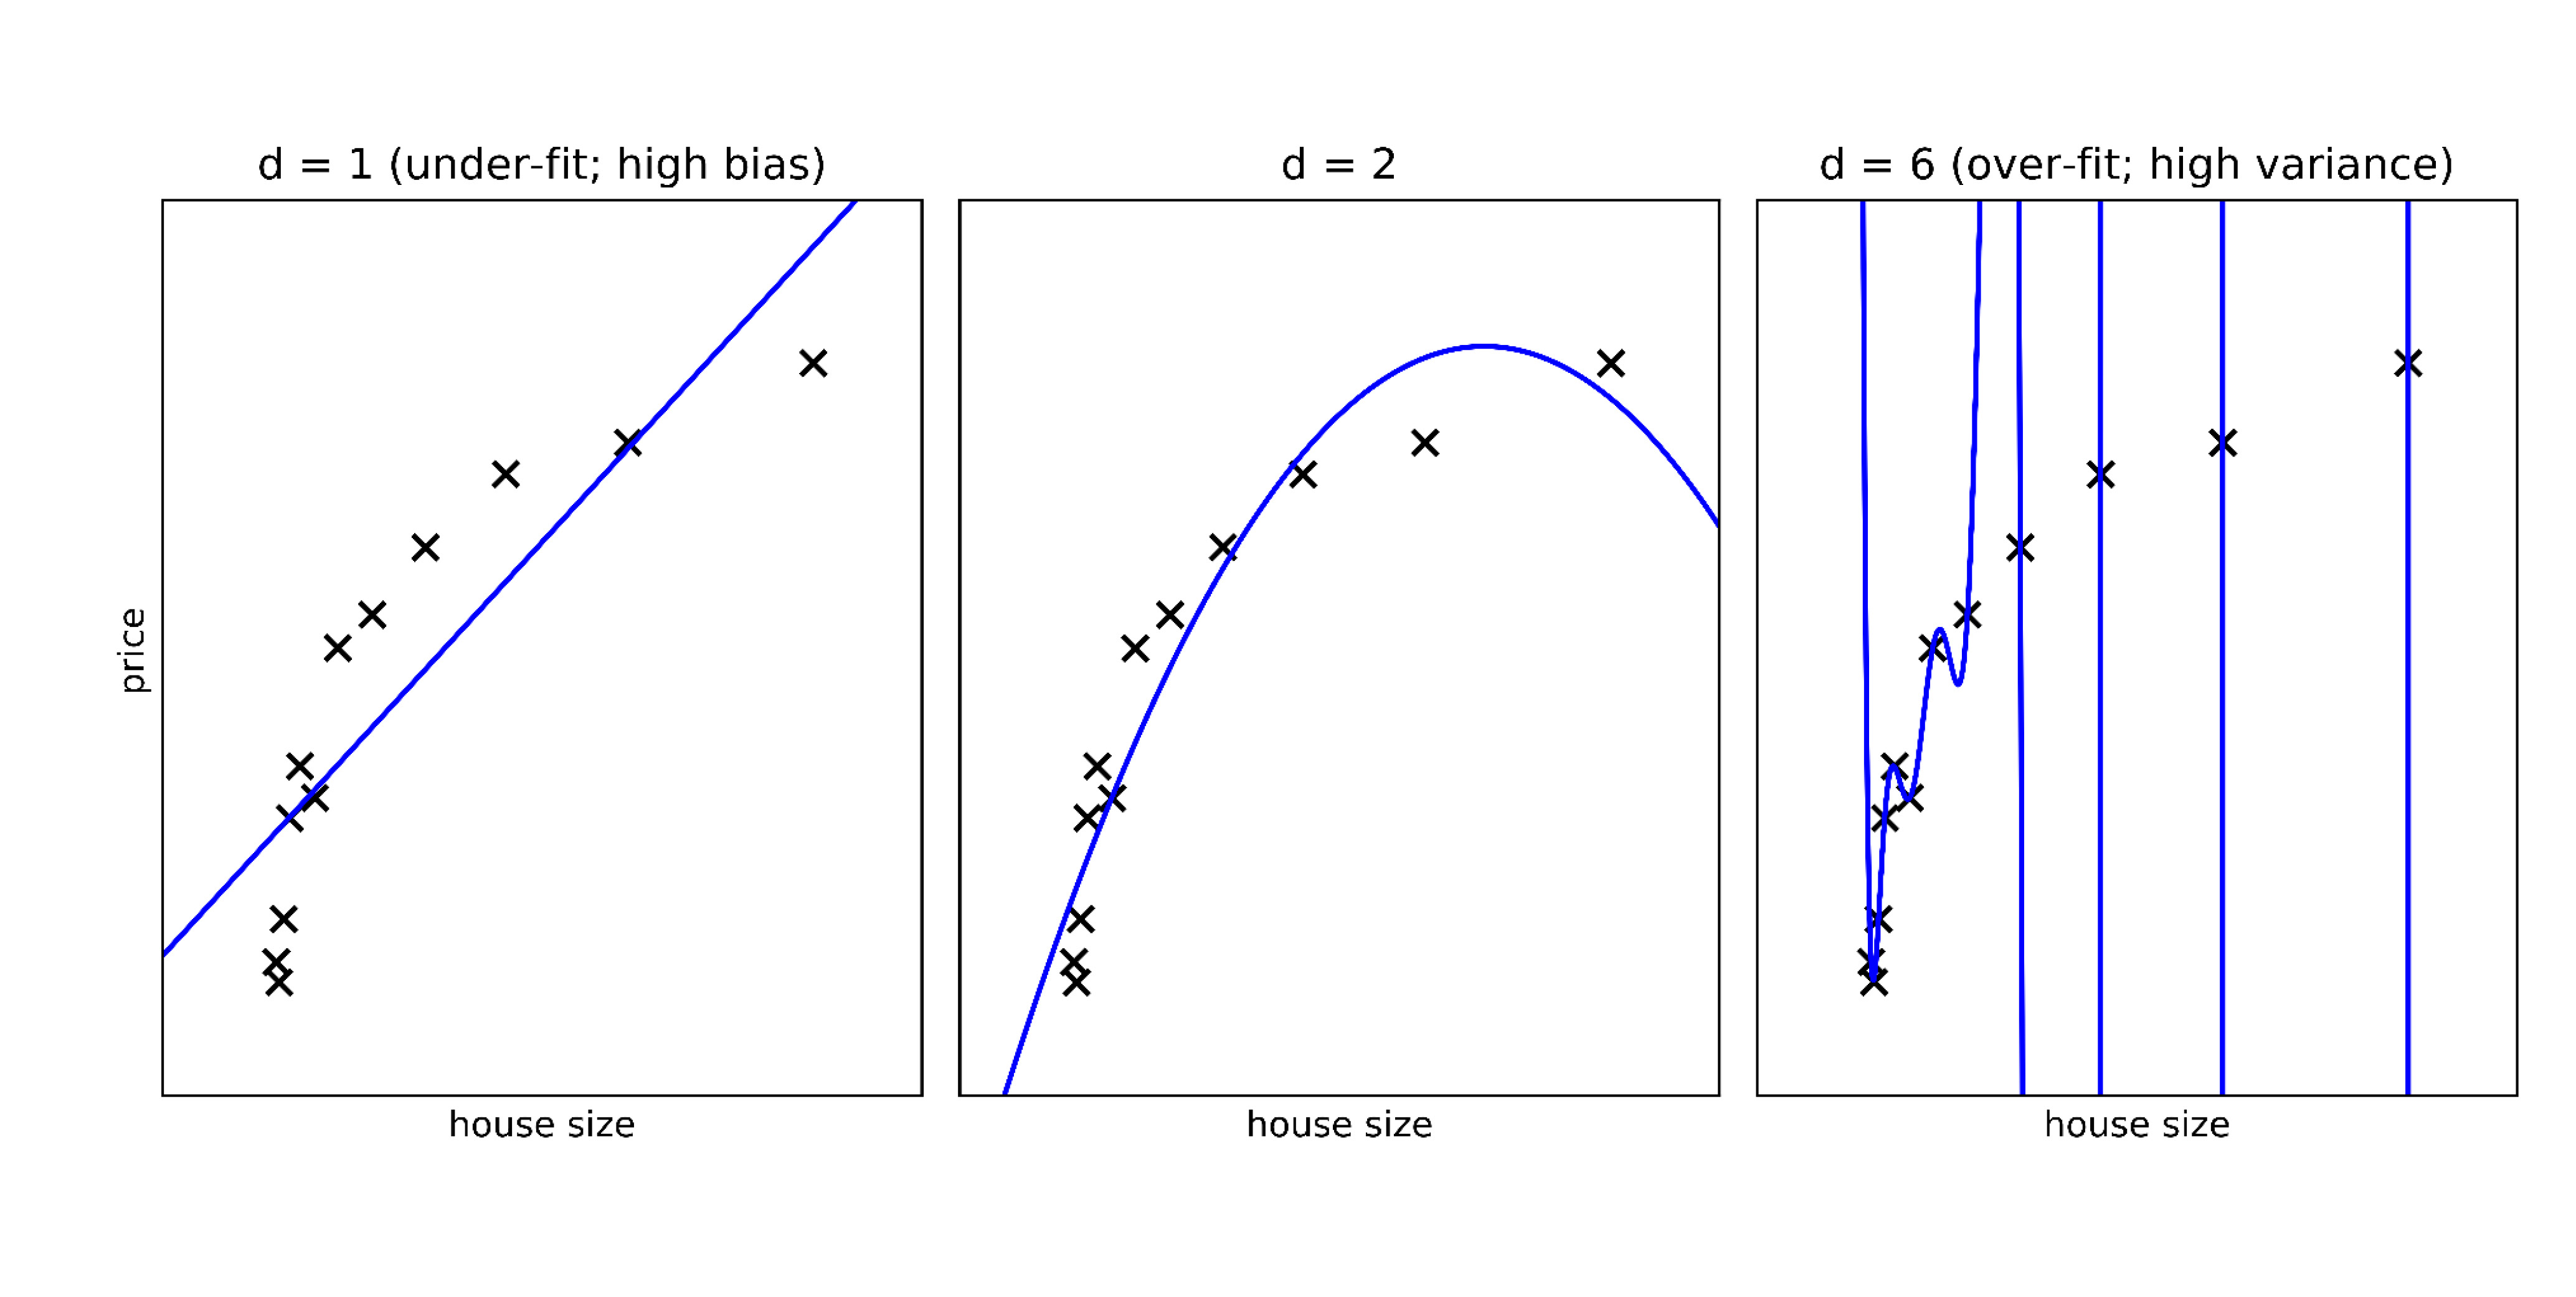
\includegraphics[width=0.8\linewidth]{img/bias_variance_tradeoff}
\end{center}

\subsection{Polynomial Regression using sklearn.pipeline}
\begin{minted}[linenos]{python}
from sklearn.pipeline import make_pipeline
from sklearn.linear_model import LinearRegression
from sklearn.preprocessing import PolynomialFeatures

model = make_pipeline(PolynomialFeatures(degree),
LinearRegression())
model.fit(x[:, np.newaxis], y)
ax.plot(x_test, model.predict(x_test[:, np.newaxis]), '-b')
\end{minted}

\subsection{Bias-Variance-Decomposition}
When the relationship between the predictor variable $X$ and the response variable $Y$ is written as
\begin{equation*}
	Y=f(X) + \epsilon \qquad \epsilon\sim\N{0,\sigma_{\epsilon}}
\end{equation*}
Then the expected value of the quadratic error can be written as
\begin{equation*}
	\text{SE}(x) = \ev{(Y - \hat{f}(x))^2}
\end{equation*}
Transformed
\begin{equation*}
	\text{SE}(x) = \underbrace{\left(\ev{\hat{f}(x)} - f(x)\right)^2}_{\text{Bias}^2} + \underbrace{\ev{\left(\hat{f}(x) - \ev{\hat{f}(x)}\right)^2}}_{\text{Variance}} + \underbrace{\sigma_{\epsilon}^2}_{\text{irreducible error}}
\end{equation*}

\subsection{The No-Free-Lunch Theorem (Probably Approximately Correct Theory)}
\begin{theorem}
	For every learner, there exists a task on which it fails, even though that task can be successfully learned by another learner.
\end{theorem}
Intuitively, as in the real world a learner is never trained on the whole data that exists, but only a subset of that data.

\subsection{Cross-Validation}
\begin{center}
	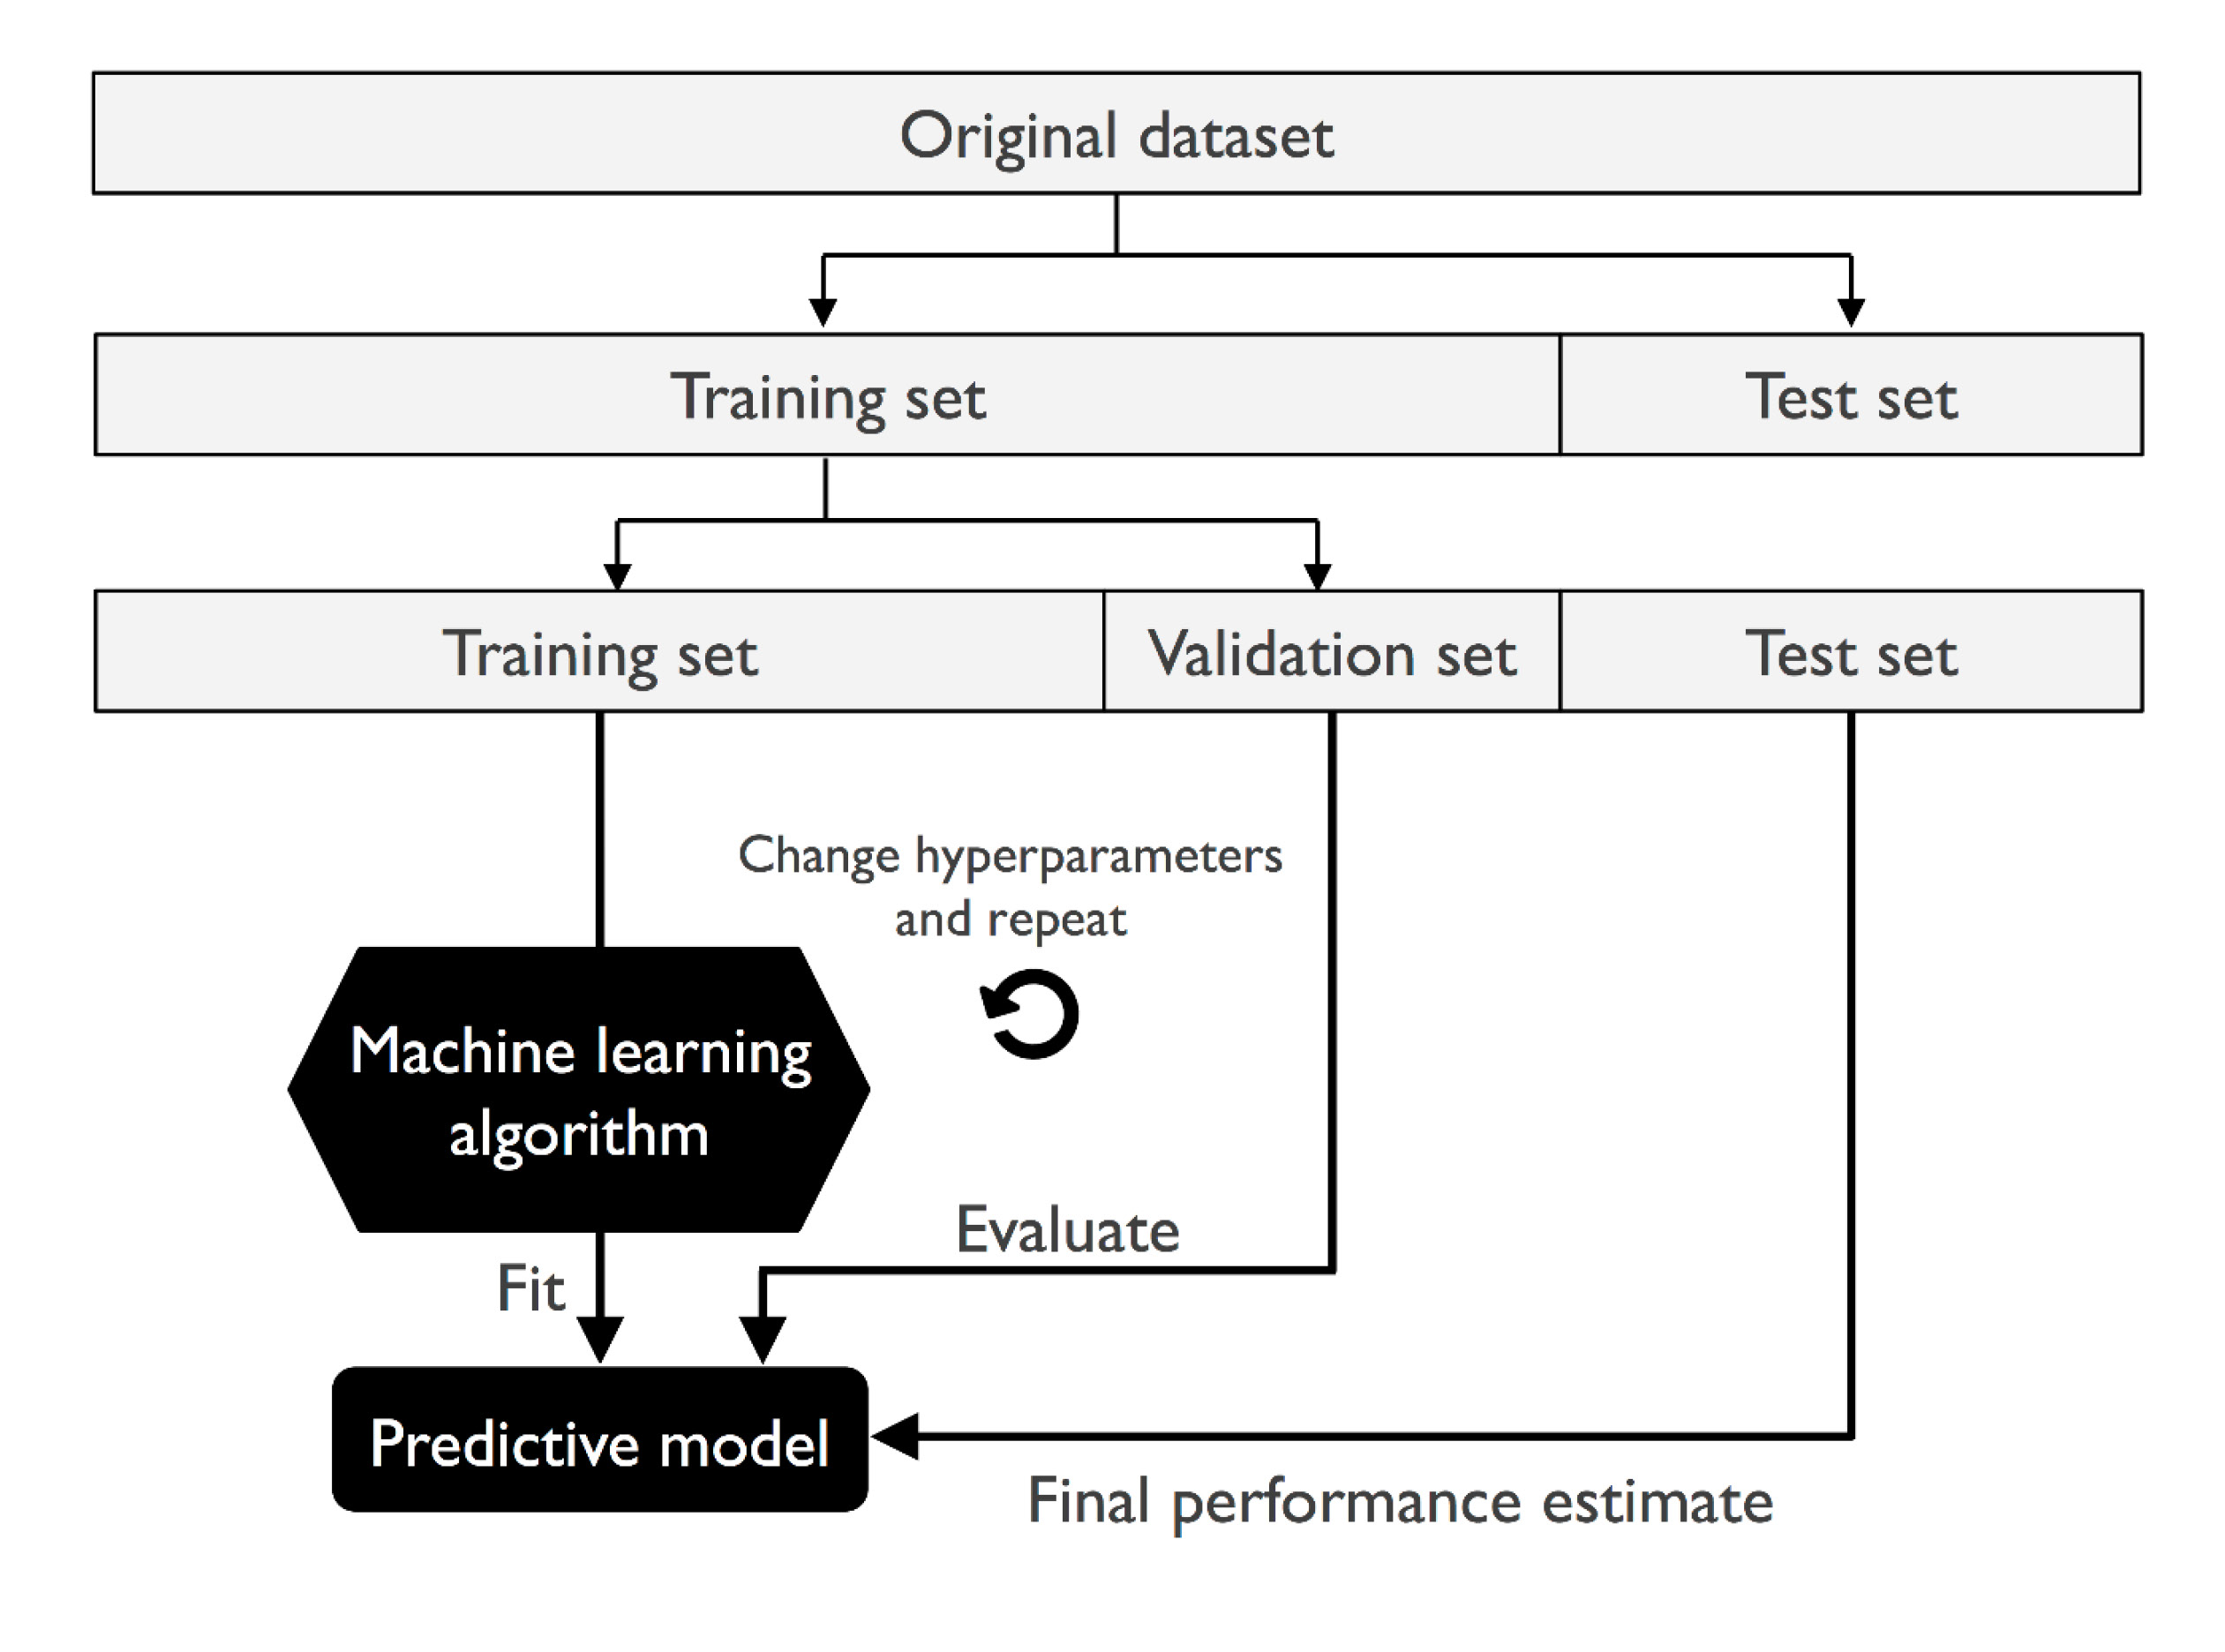
\includegraphics[width=0.7\linewidth]{img/cross_validation_hyperparameter_tuning}
\end{center}
\subsubsection{Stratified k-Fold Cross Validation for Unequal Classes}
In cases where classes are unevenly distributed, {\color{DodgerBlue3} stratified k-fold cross-validation} reduces bias and variance of the estimation. The implementation takes care to ensure that the classes are distributed approximately equally in the subsets. This ensures that the individual subsets are representative of the class distribution in the training data set.

\begin{minted}[linenos,fontsize=\small]{python}
from sklearn.model_selection import validation_curve

degrees = np.arange(1, 14)
model = make_pipeline(PolynomialFeatures(), LinearRegression())
# The parameter to vary is the "degrees" on the pipeline step "polynomialfeatures"

train_scores, validation_scores = validation_curve(
	model, x[:, np.newaxis],
	y,
	param_name='polynomialfeatures__degree',
	param_range=degrees)
\end{minted}

\subsubsection{Cross-Validated Grid Search in Python}
A grid search consists of
\begin{itemize}[nosep,noitemsep]
	\item an \textbf{estimator}
	\item a \textbf{parameter space}
	\item a method for searching or \textbf{sampling} candidates;
	\item a \textbf{cross-validation scheme}
	\item a \textbf{score function}
\end{itemize}
\begin{minted}[linenos,fontsize=\small]{python}
from sklearn import svm, datasets
from sklearn.model_selection import GridSearchCV

iris = datasets.load_iris()

parameters = {'kernel':('linear', 'rbf'), 'C':[1, 10]}
svc = svm.SVC(gamma="scale")

clf = GridSearchCV(svc, parameters, cv=5)
clf.fit(iris.data, iris.target)

sorted(clf.cv_results_.keys())
\end{minted}

\subsection{Learning Curves}
\begin{center}
	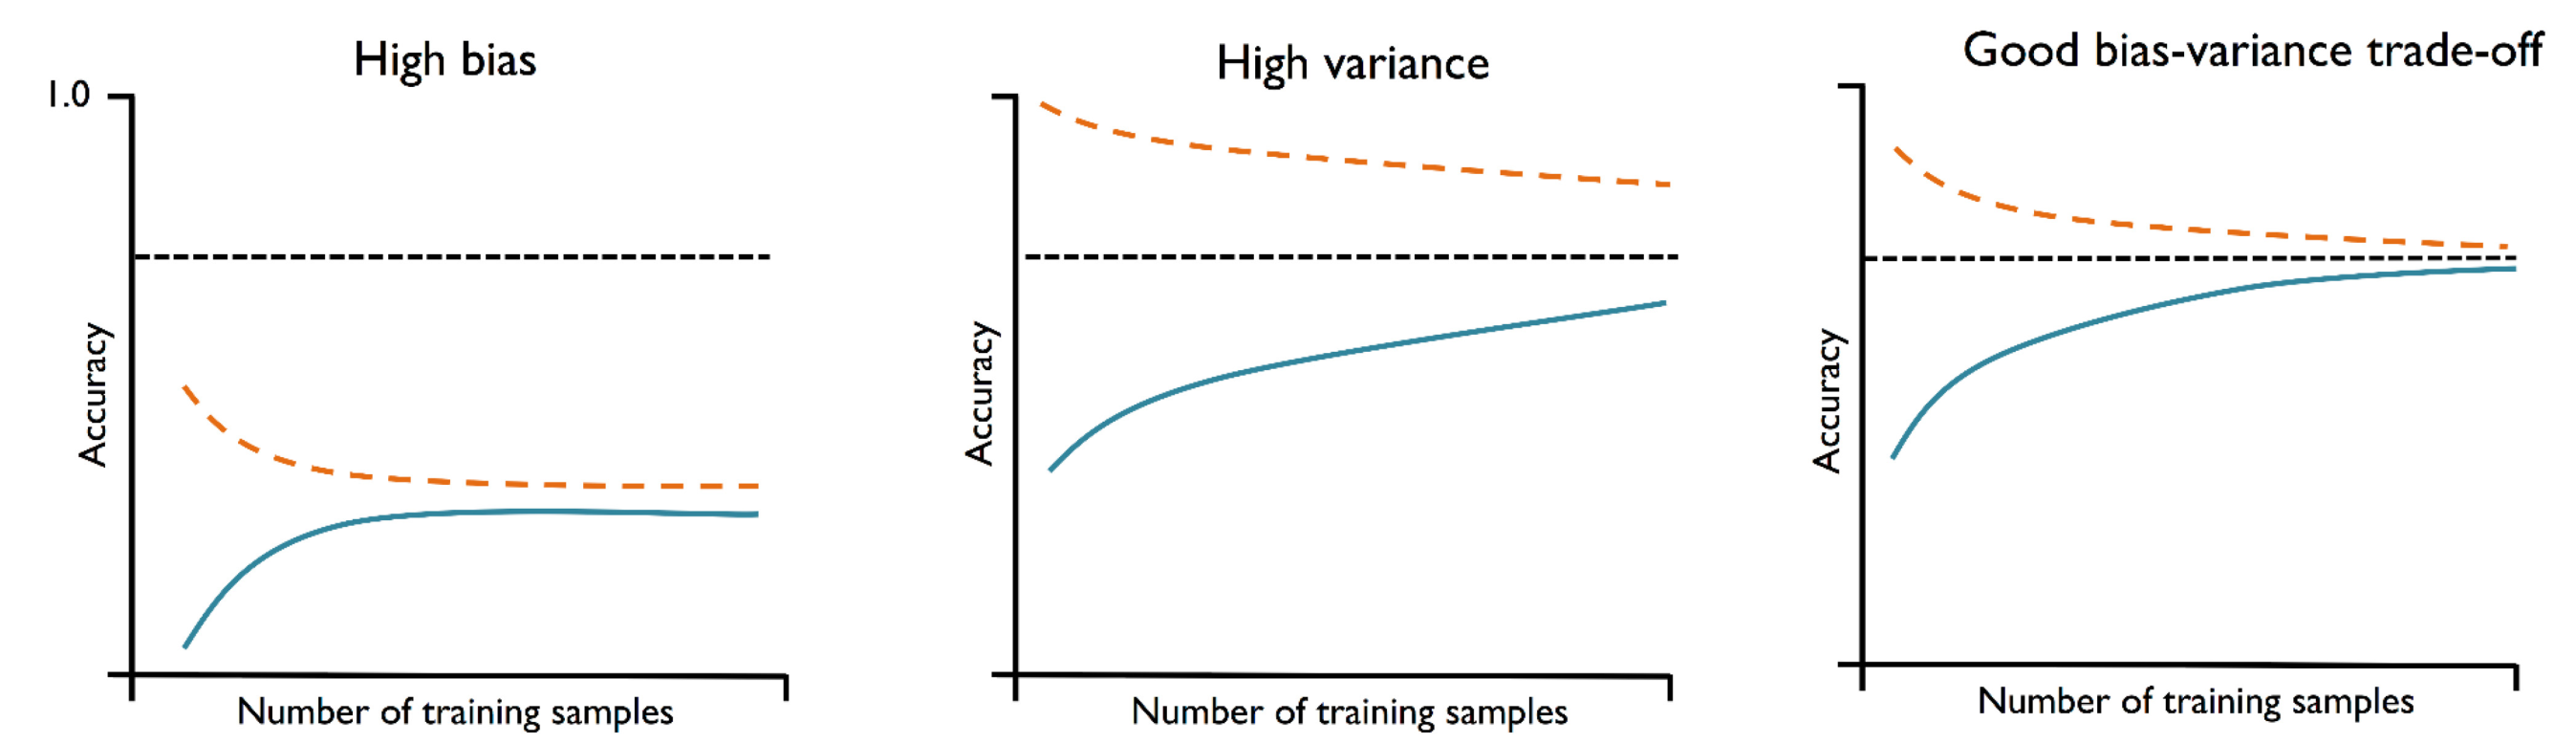
\includegraphics[width=0.9\linewidth]{img/learning_curve_bias_variance}
\end{center}
A \textbf{high bias} points to a systemic error or underfit, choose another model to approximate the real function. A \textbf{high variance} points to instability or overfit, getting more data or use more regularisation.
\subsection{Regularisation}
Ridge-Regression ($L_2$-Regression) \textbf{distributes weight} across related features and has an analytic solution
\begin{equation*}
	R_{\text{Ridge}}(\theta) = \sum_{i=1}^{d} \theta_i^2
\end{equation*}
LASSO Regression ($L_1$-Regression) encourages sparsity by setting some weights to zero and is used to select \textbf{informative features}
\begin{equation*}
	R_{\text{LASSO}}(\theta) = \sum_{i=1}^d\abs{\theta_i}
\end{equation*}

\subsection{Reduction of the Model Complexity}
Increasing the complexity of a model usually increases its variance and lowers its bias. Conversely, a lower complexity of the model increases its bias and lowers its variance. Therefore, this is called equilibrium. Regularising the model, by restricting it in some manner, is one way to avoid overfitting: The less freedom the model has, the more difficult it becomes to overfit the data. For example, a polynomial model can easily be regularised by reducing the degree of the polynomial.

\subsubsection{Minimisation of the Loss Function with Regularisation}
\begin{align*}
	L(\theta) &= \sum_{i=1}^{N} \left( y_i - \hat{y}_i(\theta) \right)^2 + \lambda \norm{\theta}_R\\
	\norm{\theta}_R:\qquad \norm{\theta}_2^2 &= \sum_{i=1}^{n} (\theta_k)^2\qquad \text{Ridge-Regression}\\
	\norm{\theta}_1 &= \sum_{i=1}^{n} \abs{\theta_k}\qquad \text{LASSO-Regression}\\
\end{align*}
with $\lambda$ being the Regularisation hyperparameter. By assigning larger values to the hyper parameter $\lambda$, we increase the regularisation strength and reduce the weights of our model. LASSO is an approach that can lead to sparse models. Depending on the regularisation strength, certain weights can become zero, which means that LASSO can also function as a \textbf{monitored feature selection procedure}.

\section{System Design}
Machine Learning systems as a whole are pipelines composed of individual components, that can be developed collaboratively as a team.

\subsection{Ceiling Analysis}
\begin{enumerate}[noitemsep,nosep]
	\item {\color{Tomato2} Baseline}: Measure the performance of the complete pipeline
	\item Replace {\color{Goldenrod1} first component} with the ground truth (perfect result for this stage) and measure performance of the system
	\item Replace {\color{OliveDrab3} next component} with the ground truth and measure performance of the system
	\item \qquad $\vdots$
\end{enumerate}
\begin{figure}[H]
	\centering
	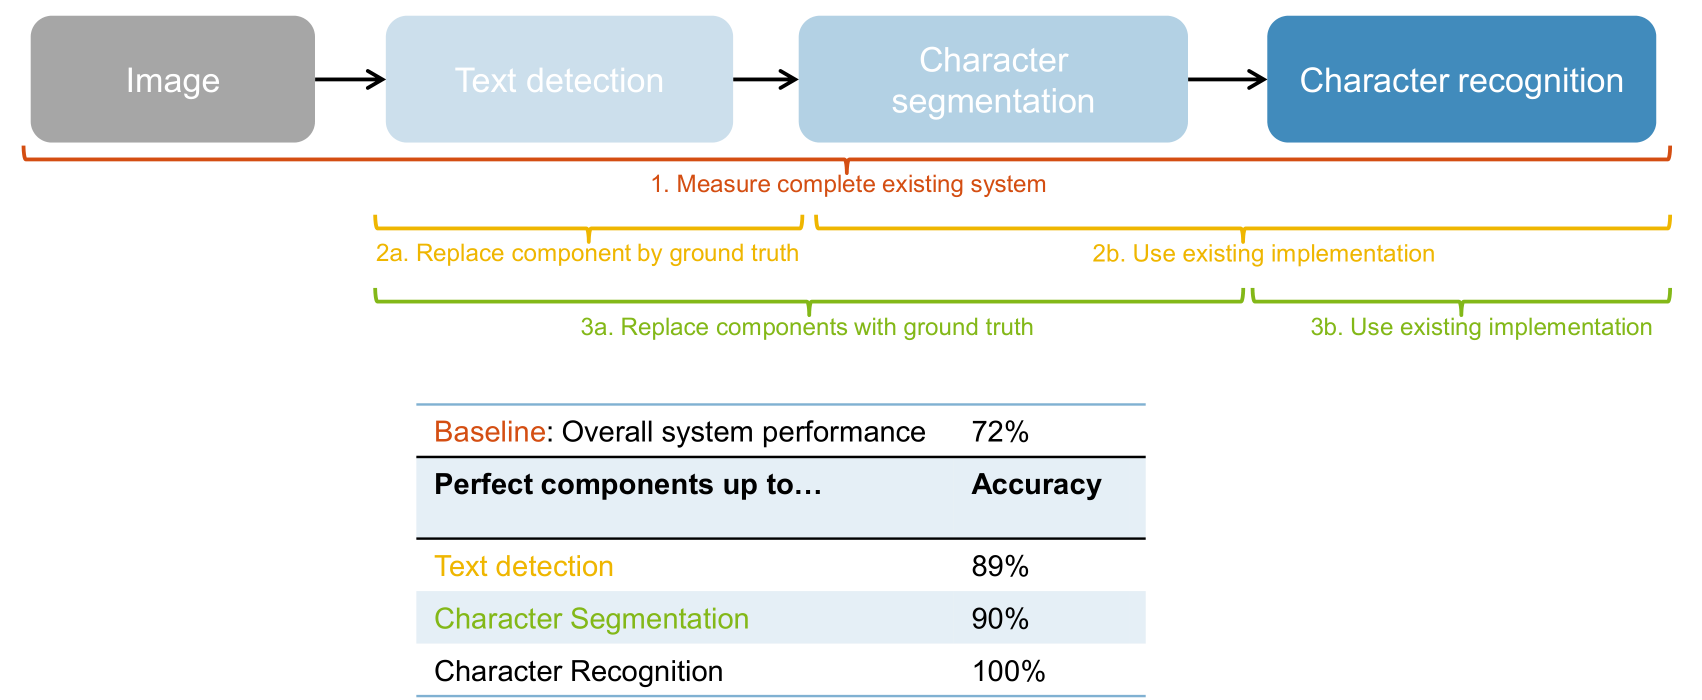
\includegraphics[width=\linewidth]{img/ceiling_analysis.png}
	\caption{Based on this analysis to improve Text Detection and Character Recognition makes sense, Character Segmentation only improves the overall performance by 1\% and is thus not worth the investment}
\end{figure}

\section{Feature Engineering}
A feature is an individual measurable property of a phenomenon being observed.

\subsubsection{Exploratory Data Analysis}
Whether collected by your workgroup or obtained from someone else, raw data is seldom ready for immediate analysis. Exploratory data analysis can help in discovering important anomalies, identifying limitations in the collection process, and to better inform subsequent goal oriented analysis.

Before generating features for the model, identify key properties of the data including structure, granularity, faithfulness, temporality and scope. This can be done by preparing, analysing and visualising the data using Histograms, QQ-Plots, Scatter-matrices and Heatmaps.

\subsubsection{Data Cleansing}
\begin{minted}{python}
# drop duplicates, drop not available
df.drop_duplicates()
df.dropna()

# replace the cells without any data in the column with the value 'None'
df = df.astype(object).where(pd.notnull(df),None)
weekday_counts = df.groupby('weekday').aggregate(sum)

# replace * in Name with empty string:
df['Name']=df['Name'].apply(lambda x:str(x).replace('*',''))

# convert dates to datetime, keeping only the month
df['MonthYear'] = pd.to_datetime(df['MonthYear'])
df['MonthYear'] = df['MonthYear'].apply(lambda x: x.date())
\end{minted}

\subsection{Feature Preparation}
\begin{itemize}
	\item \textbf{Data Cleaning}\\
	Homogenise missing values and different types of in the same feature, fix input errors, types, etc.
	\item \textbf{Aggregating / Pivoting}\\
	necessary when the entity to model is an aggregation from the provided data.
	\item \textbf{Imputation of missing values}\\
	Strategies: mean, median, mode, using a model
	\item \textbf{Binarisation}\\
	transform discrete or continuous numeric features into binary features
	\item  \textbf{Binning}\\
	Fixed width, adaptive quantile binning
	\item \textbf{Transformation}\\
	Compress the range of large numbers or expand the range of small numbers.
	\item \textbf{Scaling and normalisation}
	\item \textbf{Generate Interaction features}
\end{itemize}

\subsubsection{Box-Cox-Transformation}
\begin{minipage}{0.5\linewidth}
	The Box-Cox Transformation can be used to symmetrize positive numerical features
	\begin{equation*}
		\tilde{x}_i = \left\{ \begin{matrix}
		\frac{x_i^\lambda - 1}{\lambda} & \text{if }\lambda\neq 0\\
		\log(x_i) & \text{otherwise}
		\end{matrix} \right.
	\end{equation*}
\end{minipage}
\begin{minipage}{0.5\linewidth}
	\begin{center}
		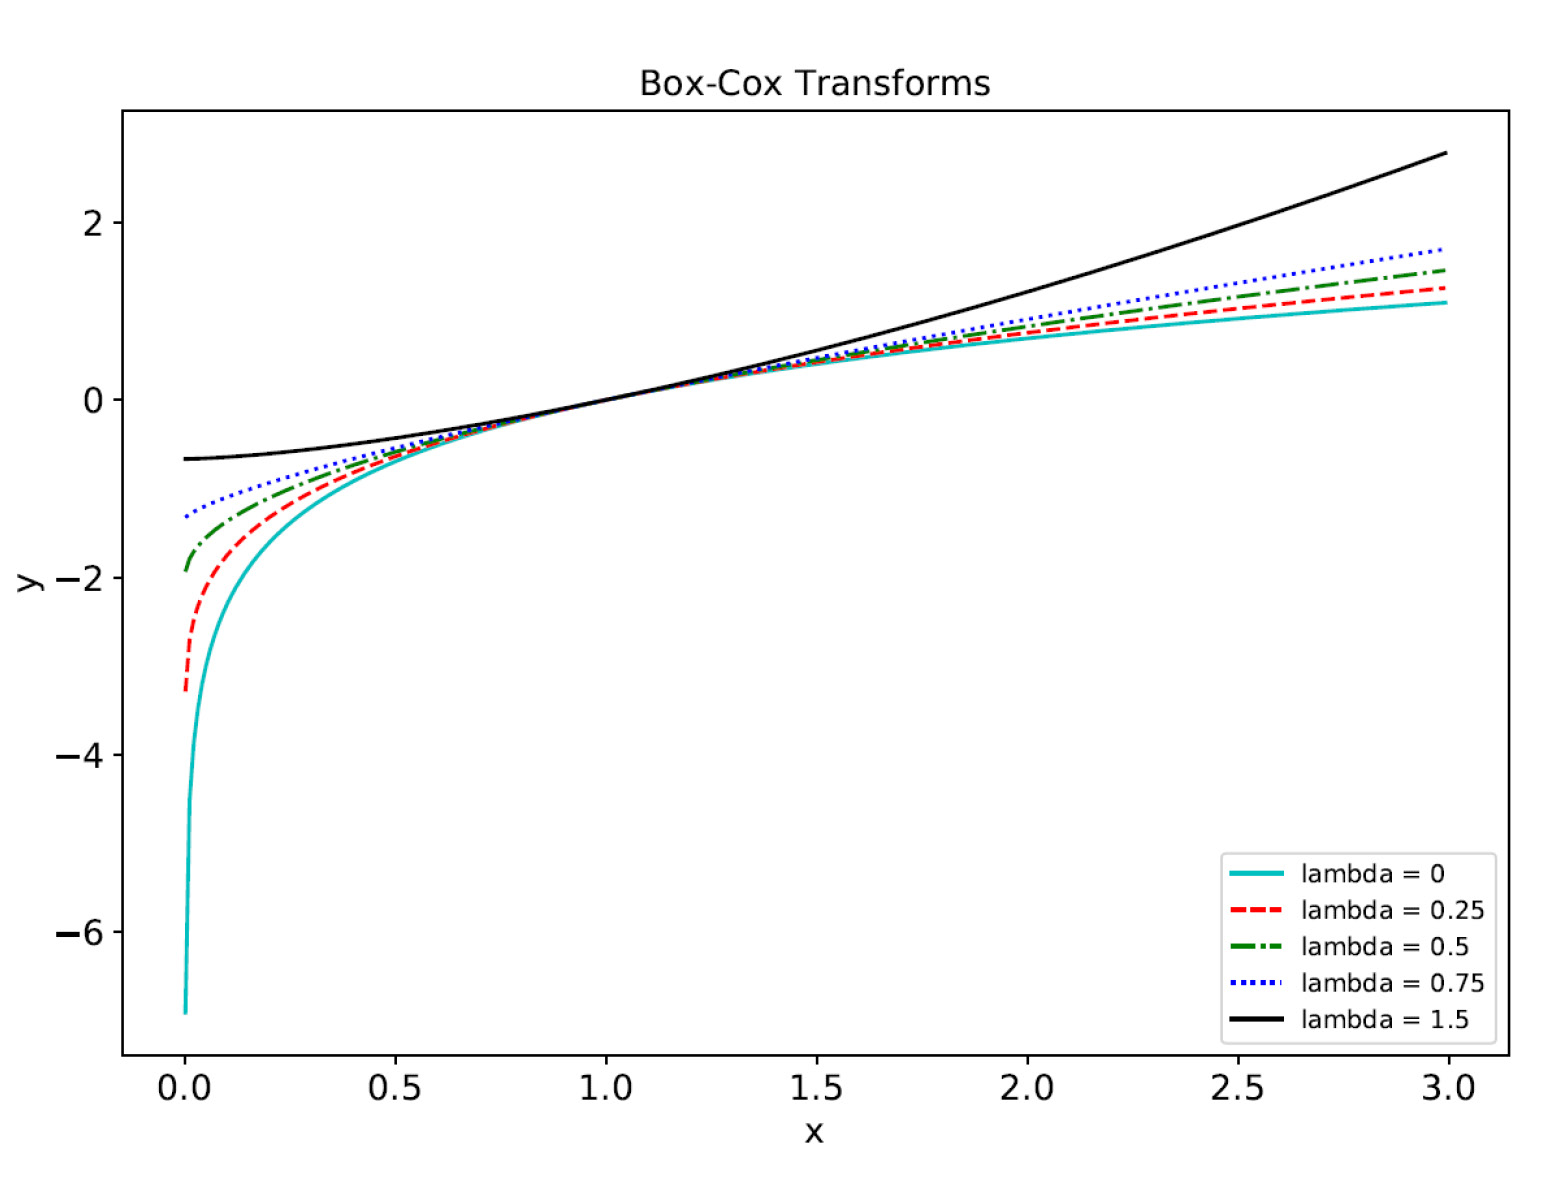
\includegraphics[width=0.9\linewidth]{img/boxcox_lambdas}
	\end{center}
\end{minipage}
\begin{minted}{python}
from sklearn.preprocessing import PowerTransformer

# select numeric features
weather_num = weather.select_dtypes(include =["float"]) #
# 'yeo-johnson' (default), works with positive and negative values
# 'box-cox', only works with strictly positive values
PowTrans = PowerTransformer(method='yeo-johnson')
# fit and transform data
weather_num_t = PowTrans.fit_transform(weather_num)
\end{minted}

\subsection{Feature Preparation}
\subsubsection{One-Hot Encoding}
\begin{minted}{python}
from sklearn.preprocessing import OneHotEncoder
enc = OneHotEncoder(handle_unknown='ignore')
X = [['Male', 1], ['Female', 3], ['Female', 2]]
enc.fit(X)
\end{minted}

\subsubsection{Bin Counting}
\begin{minted}{python}
rnd = np.random.RandomState(42); X = rnd.uniform(-3, 3, size=100)
y = np.sin(X) + rnd.normal(size=len(X)) / 3
X = X.reshape(-1, 1)
enc = KBinsDiscretizer(n_bins=10, encode='onehot')
X_binned = enc.fit_transform(X)
\end{minted}

\subsubsection{Label Encoding}
\begin{minted}{python}
le = preprocessing.LabelEncoder()
le.fit(["paris", "paris", "tokyo", "amsterdam"])
list(le.classes_)
> ['amsterdam', 'paris', 'tokyo']
le.transform(["tokyo", "tokyo", "paris"])
> array([2, 2, 1])
\end{minted}

\subsubsection{Note on NLP}
This section is covered in 'Analysis of Text Data' in much more detail, and has thus been omitted.

\subsection{Feature Selection}
The reason to use feature selection is reducing the number of features, to reduce overfitting and improve the generalization of models, and to gain  a better understanding of the features and their relationship to the response variables.

\subsection{Feature Selection using Linear Models and Regularisation}
Utilise machine learning models for feature ranking as many have some inherent internal ranking feature. Even simple linear regression
models can work when the data is not very noisy and the features are independent.

To avoid a multicollinearity problem either L1 (Lasso) or L2 (Ridge) regularisation should be used.

\begin{minted}{python}
from sklearn.linear_model import Lasso
from sklearn.preprocessing import StandardScaler
from sklearn.datasets import load_boston

boston = load_boston()
scaler = StandardScaler()
X = scaler.fit_transform(boston['data'])
Y = boston['target']
names = boston['feature_names']

lasso = Lasso(alpha=.3)
lasso.fit(X,Y)
\end{minted}
\texttt{Lasso model: -3.707 * LSTAT + 2.992 * RM + -1.757 * PTRATIO + -1.081 * DIS\\
	+ -0.7 * NOX + 0.631 * B + 0.54 * CHAS + -0.236 * CRIM + 0.081 * ZN\\
	+ {\color{red} -0.0 * INDUS} + {\color{red} -0.0 * AGE} + {\color{red}0.0 * RAD} + {\color{red}-0.0 * TAX}}
L2 or Ridge regularisation squares the coefficients in the penalty expression. This forces the coefficient values to be spread out more equally.

\subsection{Tree-based Methods for Feature Selection}
Random forest are popular methods due to their good accuracy, robustness and ease of use. Additionally, they provide a mean decrease purity and mean decrease accuracy.

\subsubsection{Information Gain}
\begin{equation*}
	\text{Entropy }H(T) = -\sum_{i=1}^{K} p_i\cdot\log_2(p_i)
\end{equation*}
Where $p_i$ represent the percentage of each class present in the child node that results from a split in the tree.
\begin{equation*}
	\text{Information Gain } \text{IG}(T,a) = H(T) - H(T|a)
\end{equation*}
\begin{equation*}
	\text{IG}(T,a) = -\sum_{i=1}^{K} p_i\cdot\log_2(p_i) - \sum_a p(a)\cdot\sum_{i=1}^{K} p(i|a)\cdot\log_2[p(i|a)]
\end{equation*}

\subsection{Recursive Feature Elimination (RFE)}
Given an external estimator that weighs features, RFE selects features by recursively considering smaller sets of features.

\section{Bayes' Theorem}
\subsection{Multivariate Gaussian Distribution}
Gaussian defined over a vector x of continuous variables in a D-dimensional space with mean vector $\mu$ and covariance matrix $\bm{\Sigma}$, where $ \abs{\bm{\Sigma}} $ is the determinant of $\bm{\Sigma}$.
\begin{equation*}
	p(\bm{x}) = \N{\bm{x}|\mu, \bm{\Sigma}} = \frac{1}{(2\pi)^{\frac{D}{2}} \norm{\bm{\Sigma}}^{\frac{1}{2}}} \exp\left\{ -\frac{1}{2} (\bm{x} - \mu)^T \bm{\Sigma}^{-1} (\bm{x} - \mu) \right\}
\end{equation*}
The quadratic form in the argument of the exponential is called \emph{Mahalanobis distance}
\begin{equation*}
	\bm{\Delta} = (\bm{x} - \mu)^T \bm{\Sigma}^{-1} (\bm{x} - \mu)
\end{equation*}
Without loss of generality, we can assume that $\bm{\Sigma}$ is symmetric with real eigenvalues and an orthonormal set of eigenvectors $\mu_i$.

\subsection{Probability Distribution}
Since $\bm{\Sigma}$ is real and symmetric, the eigenvectors $\lambda_i$ are real and the eigenvectors can be chosen from an orthonormal set, so that
\begin{align*}
	\textbf{u}_i^T \textbf{u}_j &= \delta_{ij}\\
	\bm{\Sigma} &= \sum_{i=1}^{D} \lambda_i \textbf{u}_i\textbf{u}_i^T\\
	\bm{\Sigma}^{-1} &= \sum_{i=1}^{D} \frac{1}{\lambda_i} \textbf{u}_i\textbf{u}_i^T\\
	\intertext{The quadratic form becomes}
	\Delta^2 &= \sum_{i=1}^{D}\frac{y_i^2}{\lambda_i}\\
	y_i &= \textbf{u}_j^T (\textbf{x} - \mu)
\end{align*}
This describes a D-dimensional ellipsoid with main axes $\sqrt{\lambda_i}$. The determinant is given by the product of the eigenvalues
\begin{equation*}
	\abs{\bm{\Sigma}}^{\tfrac{1}{2}} = \prod_{j=1}^{D} \lambda_j^{\tfrac{1}{2}}
\end{equation*}

\begin{definition}
	\begin{align*}
		\intertext{Expected Value}
		\ev{\textbf{x}} &= \bm{\mu}\\
		\intertext{Correlation}
		\ev{\textbf{xx}^T} &= \bm{\mu\mu}^T + \bm{\Sigma}\\
		\intertext{Covariance}
		\text{Cov}[\textbf{x}] &= \ev{(\textbf{x}-\ev{\textbf{x}})(\textbf{x}-\ev{\textbf{x}})^T} = \bm{\Sigma}
	\end{align*}
\end{definition}

Partition $\textbf{x}$ into two disjoint subsets $\textbf{x}_a$ and $\textbf{x}_b$. Without loss of generality, $\textbf{x}_a$ can be taken to form the first $M$ components of $\textbf{x}$ with $\textbf{x}_b$ comprising of the remaining $D-M$ components
\begin{alignat*}{4}
	\textbf{x}&=\begin{pmatrix}\textbf{x}_a\\\textbf{x}_b\end{pmatrix} &\qquad& \bm{\mu} &= \begin{pmatrix}\bm{\mu}_a\\\bm{\mu}_b\end{pmatrix} &\qquad& \bm{\Sigma} &= \begin{pmatrix}\bm{\Sigma}_aa & \bm{\Sigma}_ab \\\bm{\Sigma}_ba & \bm{\Sigma}_bb\end{pmatrix}
\end{alignat*}
In most situations it is more convenient to work with the \textbf{inverse of the covariance matrix}, which is called the \textbf{precision matrix}
\begin{align*}
	\bm{\Lambda} &\equiv \bm{\Sigma}^{-1}\\
	\bm{\Lambda} &= \begin{pmatrix}
		\bm{\Lambda}_{aa} & \bm{\Lambda}_{ab}\\
		\bm{\Lambda}_{ba} & \bm{\Lambda}_bb
	\end{pmatrix}
\end{align*}
The Conditional Probability Distribution of a Gaussian
\begin{align*}
	p(\textbf{x}_a| \textbf{x}_b) &= \N{\textbf{x}_a\middle| \bm{\mu}_{a|b}, \bm{\Delta}^{-1}_{aa}}\\
	\bm{\mu}_{a|b} &= \bm{\mu}_{a} - \bm{\Delta}^{-1}_{aa}\bm{\Delta}_{ab}(\textbf{x}_b-\bm{\mu}_b)\\
	&= \bm{\mu}_{a} + \bm{\Sigma}_{ab}\bm{\Delta}^{-1}_{bb}(\textbf{x}_b-\bm{\mu}_b)\\
	\bm{\Sigma}_{ab} &= \bm{\Delta}^{-1}_{aa}\\
	&= \bm{\Sigma}_{aa} - \bm{\Sigma}_{ab}\bm{\Sigma}^{-1}_{bb}\bm{\Sigma}_{ba}
\end{align*}
And the marginal probability distribution
\begin{equation*}
	p(\textbf{x}_a) = \N{\textbf{x}_a\middle| \bm{\mu}_{a}, \bm{\Sigma}_{aa}}
\end{equation*}

\subsection{Belief Networks or Bayesian Networks}
A belief network is a directed acyclic graph (DAG) in which each node has associated the conditional probability of the node given its parents. The joint distribution is obtained by taking the product of the conditional probabilities
\begin{center}
	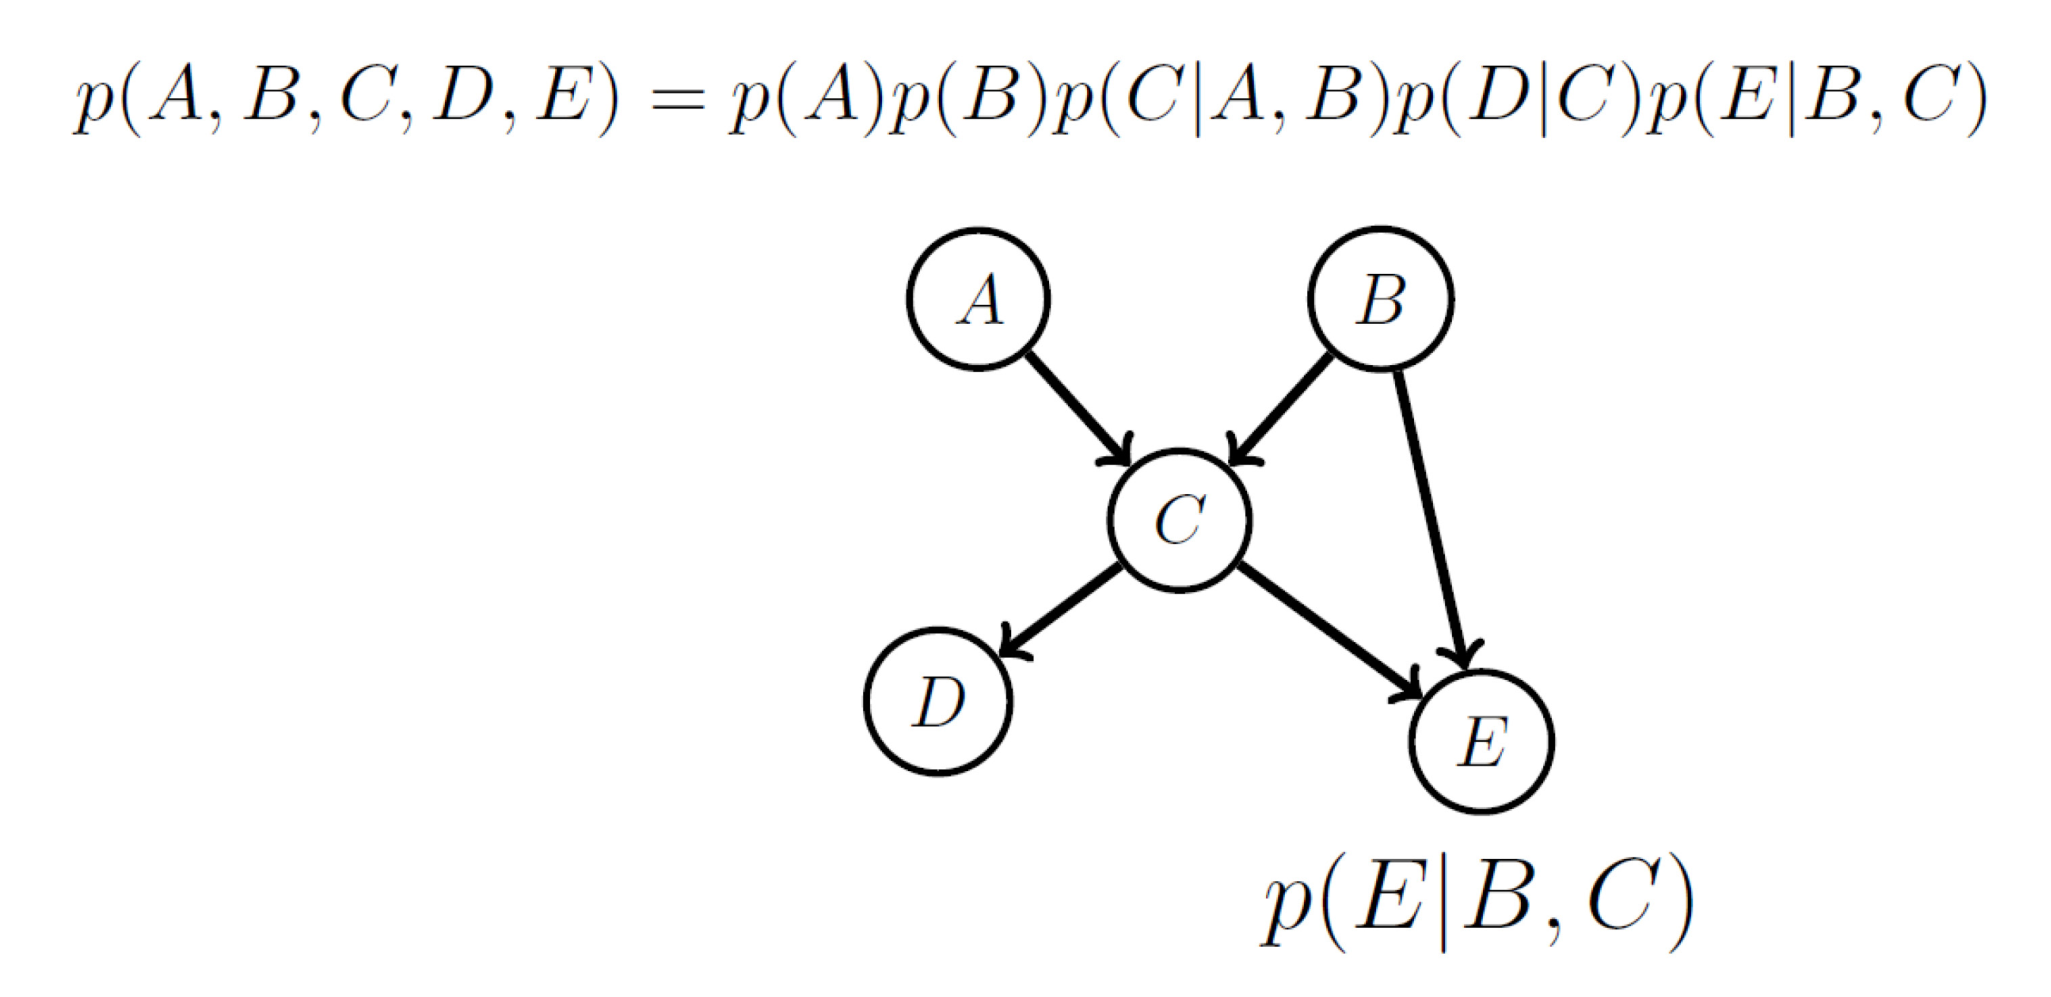
\includegraphics[width=0.7\linewidth]{img/belief_network}
\end{center}
$ \bm{X} \incond \bm{Y} | \bm{Z}$ denotes that two sets of variables $\bm{X}$ and $\bm{Y}$ are independent of each other given the state of the set of variables $\bm{Z}$. This means that
\begin{align*}
	p(\bm{X},\bm{Y}|\bm{Z}) &= p(\bm{X}|\bm{Z})\cdotp(,\bm{Y}|\bm{Z})\\
	p(\bm{X}|\bm{Y},\bm{Z}) &= p(\bm{X}|\bm{Z})
\end{align*}
for all states of $\bm{X},\bm{Y},\bm{Z}$. In case the conditioning set is empty we may also write
\begin{equation*}
	\bm{X} \incond \bm{Y}
\end{equation*}
in which case $\bm{X}$ is unconditionally independent of $\bm{Y}$.
\begin{center}
	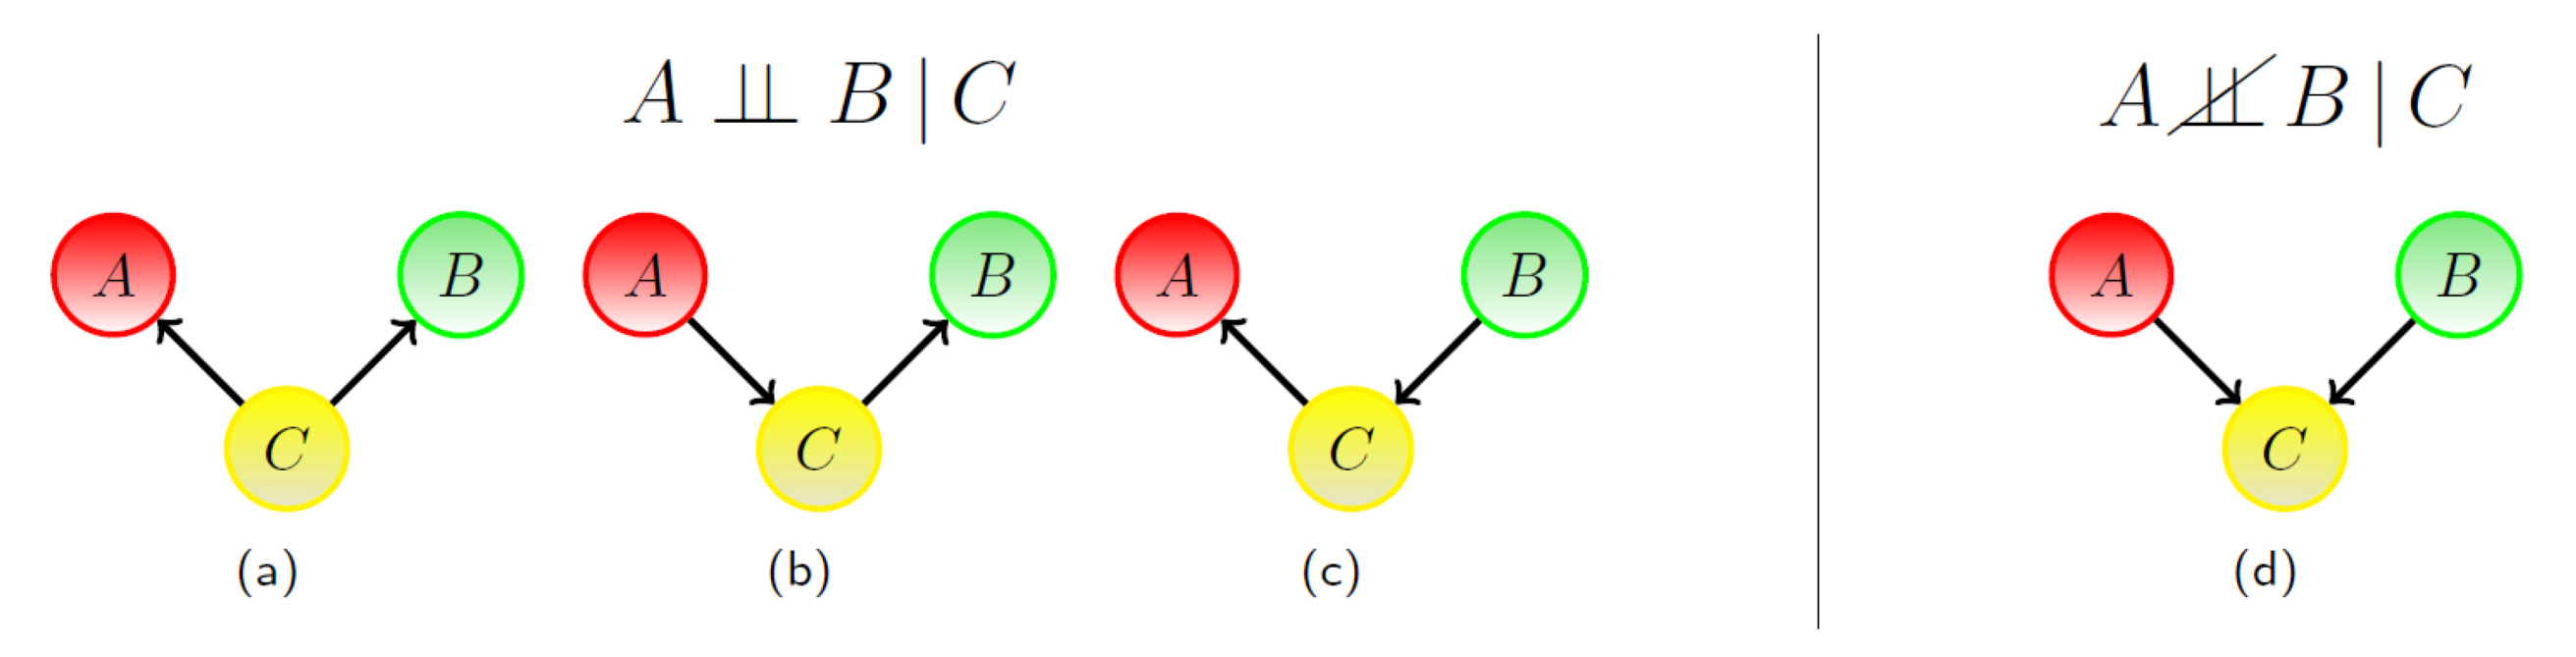
\includegraphics[width=0.7\linewidth]{img/conditional_independence}
\end{center}
In (d) the variables $A,B$ are conditionally dependent given $C$
\begin{equation*}
	P(A,B|C) \propto p(C|A,B)p(A)p(B)
\end{equation*}

\subsubsection{Collider}
A collider contains two or more incoming arrows along a chosen path.
\begin{center}
	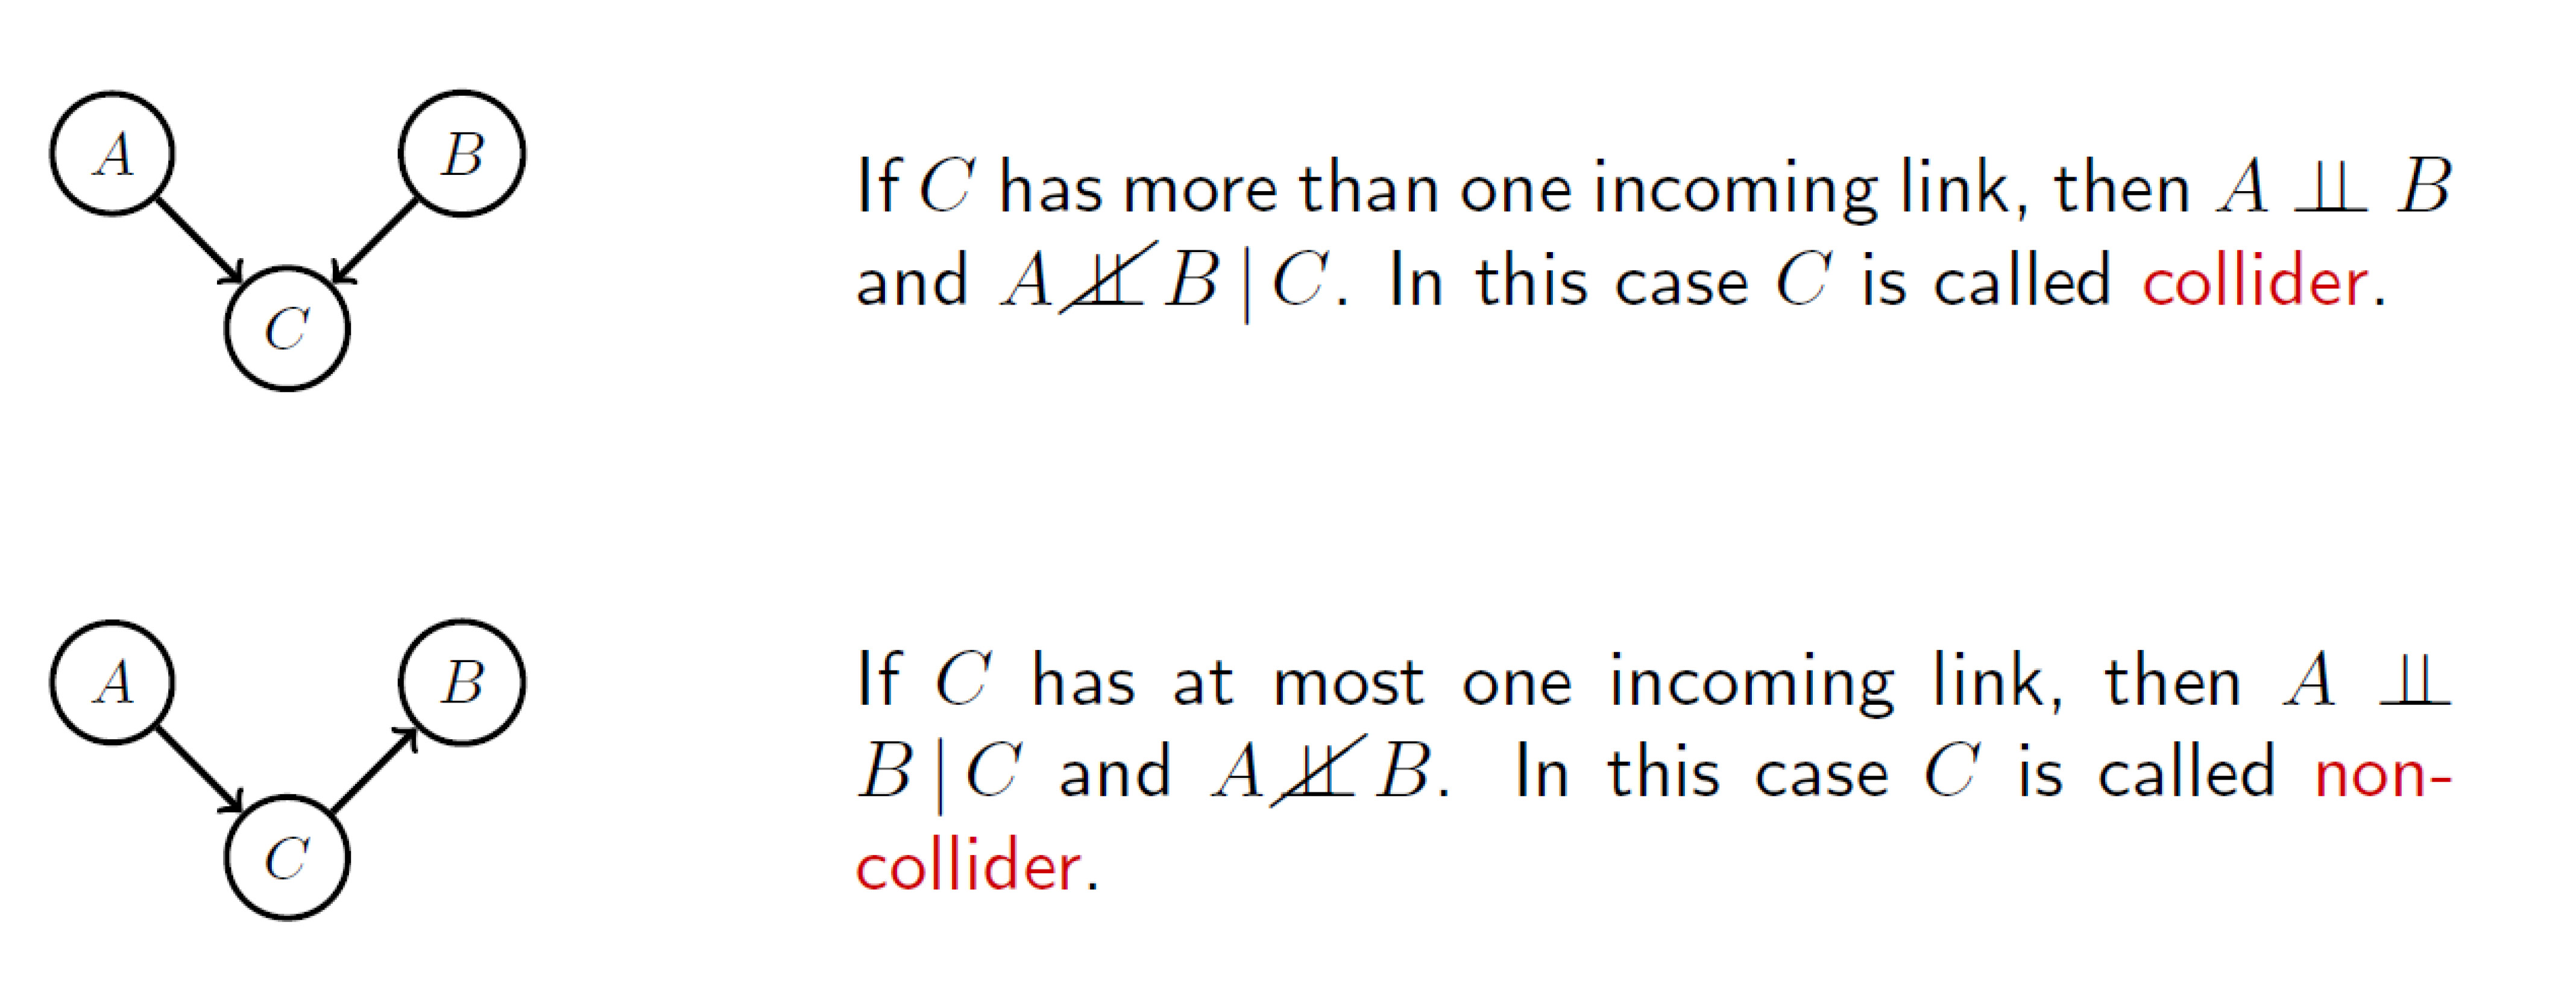
\includegraphics[width=0.8\linewidth]{img/conditional_independence_collider}
\end{center}

\subsection{Bayes' Theorem}
\begin{center}
	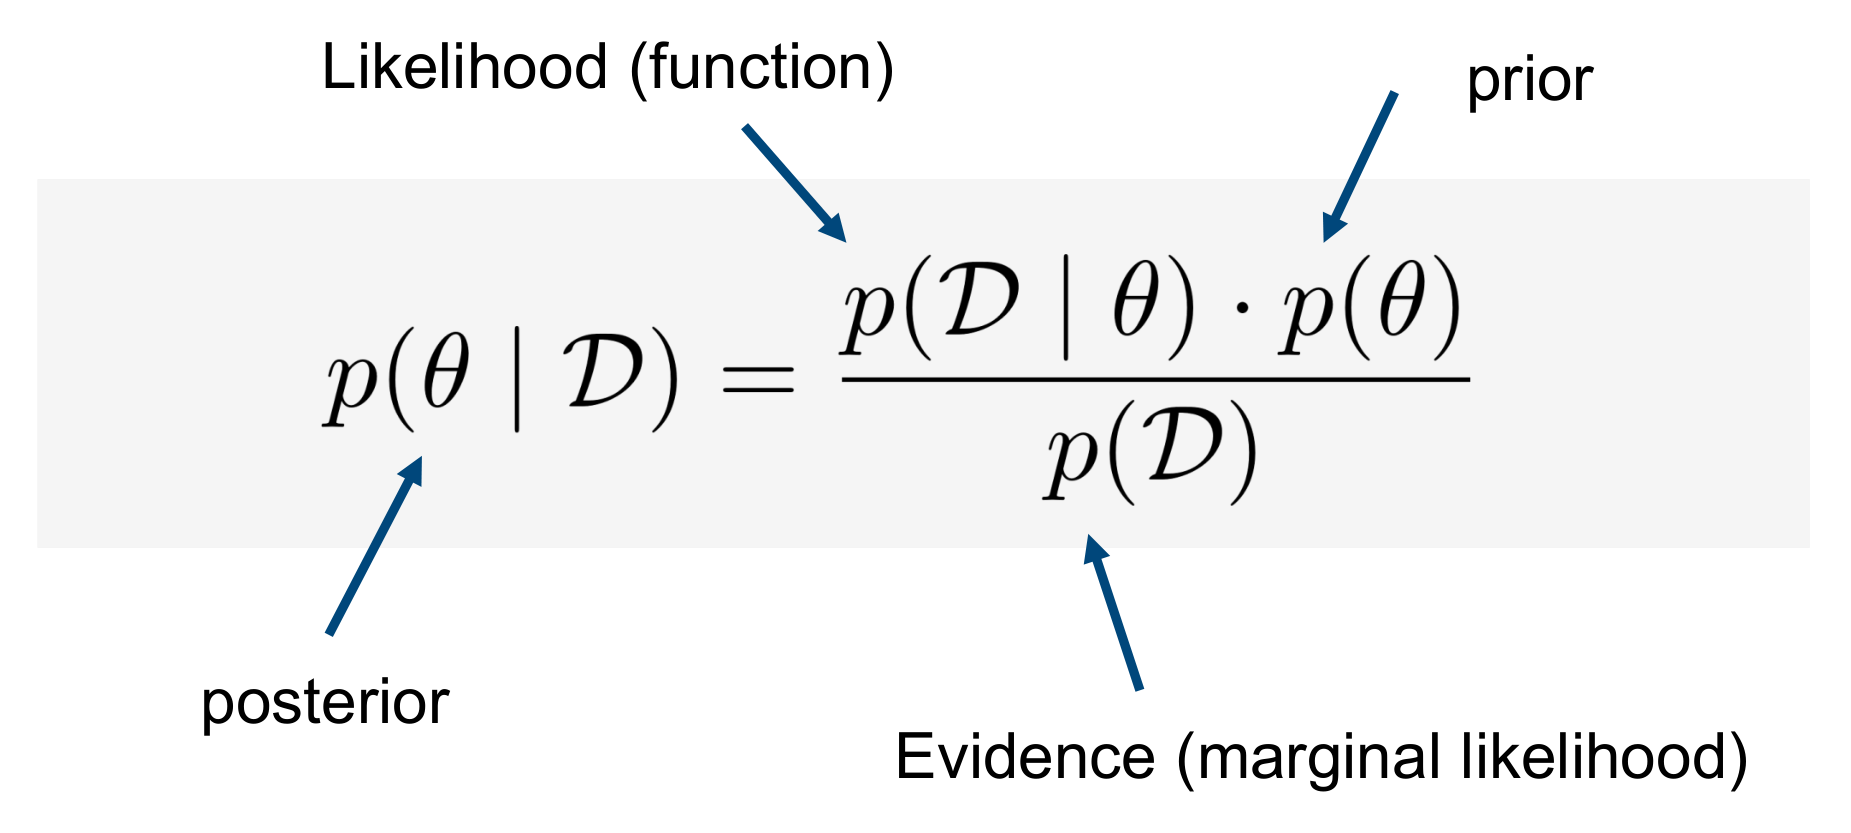
\includegraphics[width=0.6\linewidth]{img/bayes_theorem}
\end{center}

\begin{center}
	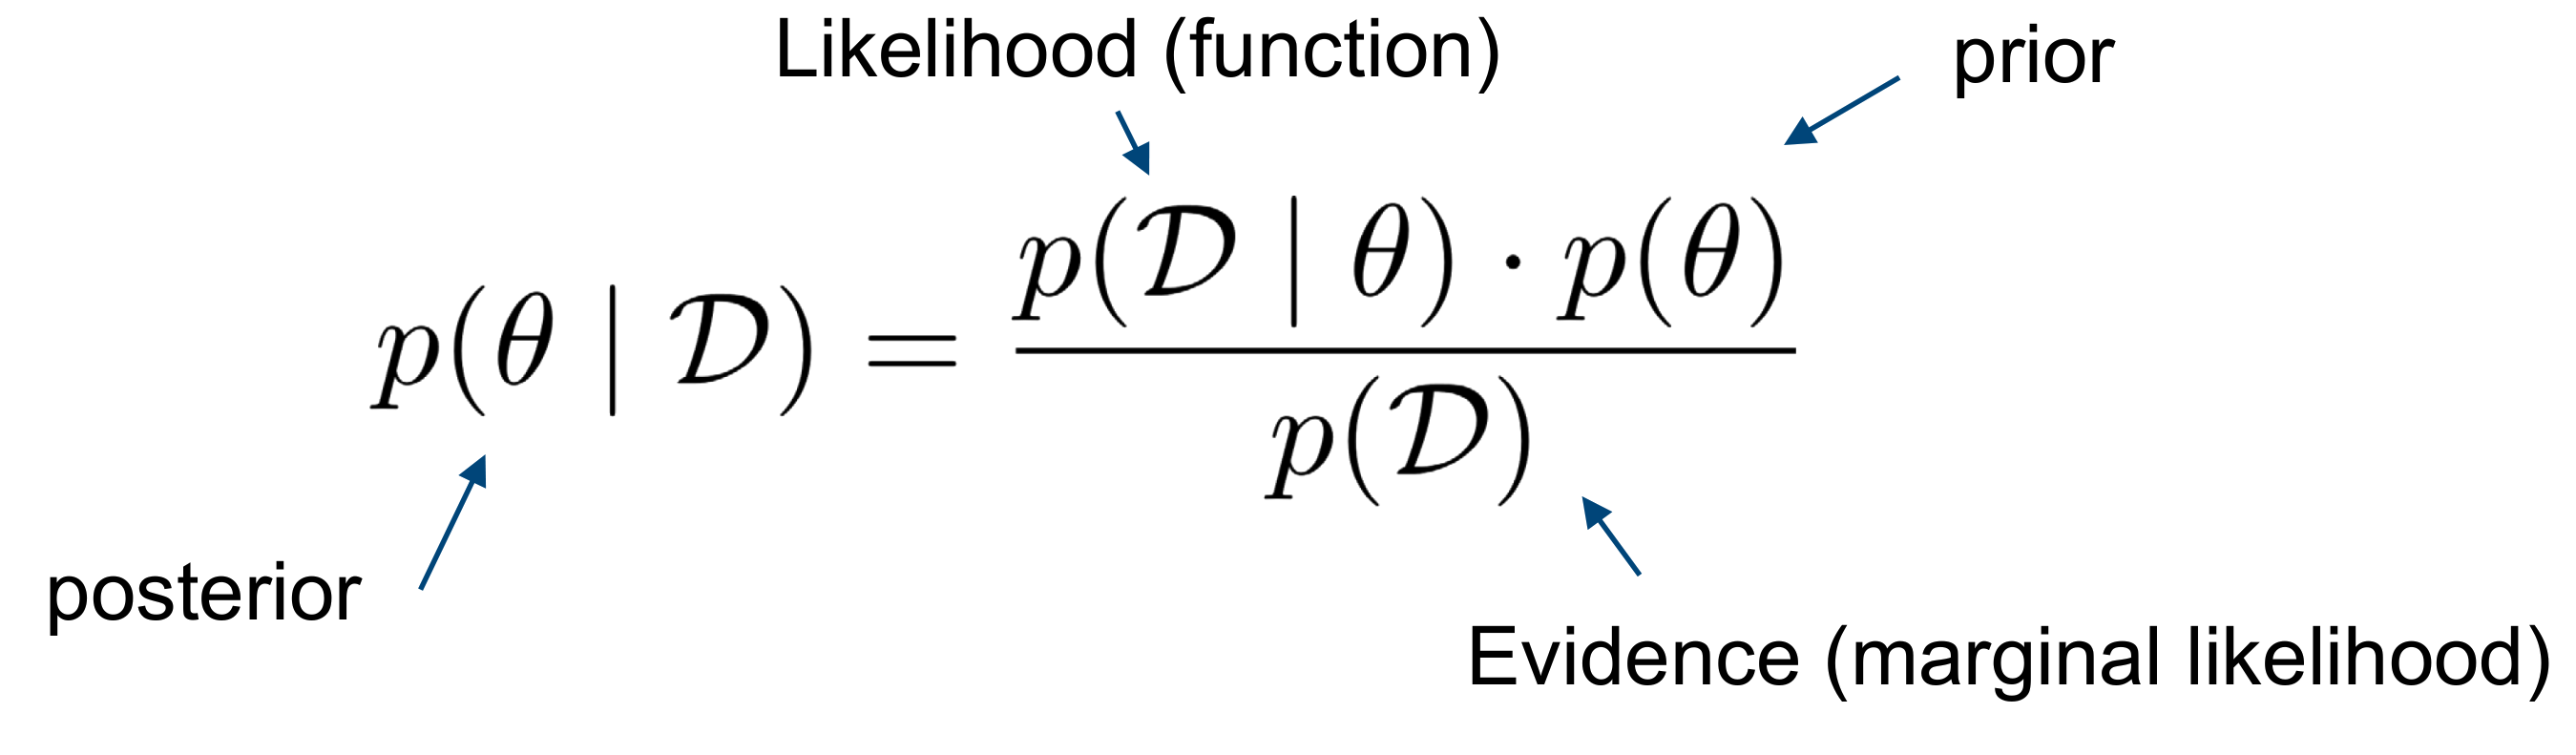
\includegraphics[width=0.7\linewidth]{img/bayes_theorem_descriptions}
\end{center}

In machine learning the condition of Bayes' theorem also includes the model $M$
\begin{equation*}
	p(\theta|D,M) = \frac{p(D | \theta, M) \cdot p(\theta | M)}{p(D|M)}
\end{equation*}
The Most probable A Posteriori (MAP) setting is that which maximises the posterior
\begin{equation*}
	\hat{\theta}_{\text{MAP}} = \argmax{\theta}\{p(\theta|D,M)\} = \argmax{\theta}\{p(\theta,D|M)\}
\end{equation*}
The Maximum Likelihood assignment is used whe $p(\theta|M)$ is constant
\begin{equation*}
	\hat{\theta}_{\text{ML}} = \argmax{\theta} \{p(\theta|D,M)\} = \argmax{\theta}\{p(D|\theta,M)\}
\end{equation*}
The Bayes optimal classifier gives the theoretically optimal classification, by combining the predictions of all hypotheses weighed by their posterior probabilities
\begin{equation*}
	Y \leftarrow \argmax{y_k} P(Y=y_k) \prod_{i} P(X_i | Y=y_k)
\end{equation*}

\section{Gaussian Processes}
Is referred to as the \textbf{infinite-dimensional extension of the multivariate normal distribution}. When we are working with Gaussian Processes the intuition is that we observe some finite-dimensional subset of infinite-dimensional data, and this finite subset follows a multivariate normal distribution, as would every finite subset.

Gaussian random variables are useful in machine learning and statistics for two main reasons.
\begin{enumerate}
	\item They are extremely common when modelling 'noise' in statistical algorithms
	\item Gaussian random variables are convenient for many analytical manipulations, because many of the integrals involving Gaussian distributions that arise in practice have \textbf{simple closed form solutions}
\end{enumerate}

\subsection{Bayesian Regression}
\begin{align*}
	\intertext{Parameter Posterior}
	p(\theta|\D) &= \frac{p(\D|\theta)\cdot p(\theta)}{\int_{\theta'} p(\D|\theta)\cdot p(\theta) \diff \theta'}
	\intertext{Posterior Predictive Distribution}
	p(y_{*}|x_{*}\D) &= \int_{\theta} p(x_{*}|y_{*},\theta)\cdot p(\theta|\D)\diff\theta
\end{align*}
\texttt{pymc3} is a comfortable package for Bayesian Inference in python.
\begin{minted}[breaklines, fontsize=\small]{python}
from pymc3 import *

with Model() as model:
    # model specifications in PyMC3 are wrapped in a with-statement
    # Define priors (#tau = precision = 1/variance = 1/sigma^2)
    sigma = HalfCauchy('sigma', beta=10, testval=1.)
    intercept = Normal('Intercept', 0, tau=1/20**2)
    x_coeff = Normal('x', 0, tau=1/20**2)
    
    # Define likelihood
    likelihood = Normal('y', mu=intercept + x_coeff * x, tau=1/sigma**2, observed=y)
    
    # Inference!
    trace = sample(3000, cores=2)
    
    # draw 3000 posterior samples using NUTS sampling
    plt.figure(figsize=(7, 7))
    traceplot(trace[100:]); plt.tight_layout();
\end{minted}

\subsection{Gaussian Processes}
\begin{equation*}
	h(\bm{x})\sim \N{\bm{m}(\bm{x}), \bm{k}(\bm{x},\bm{x}')}
\end{equation*}
\textbf{Gaussian Processes} are the extension of multivariate Gaussians to infinite-sized collections of real-valued variables. Gaussian processes can be thought of as distributions not just over random vectors but in fact distributions over random functions. A Gaussian process is a stochastic process such that any finite sub-collection of random variables has a multivariate Gaussian distribution.

In particular, a collection of random variables $ \{h(x): x\in\X\} $ is said to be drawn from a Gaussian process with \textbf{mean function $\bm{m(\cdot)}$} and \textbf{covariance function} 
$\bm{k(\cdot,\cdot)}$ if for any finite set of elements $x_1,x_2,\dots,x_m\in\X$ and the associated finite set of random variables $h(x_1), h(x_2),\dots,h(x_m)$ have a distribution
\begin{center}
	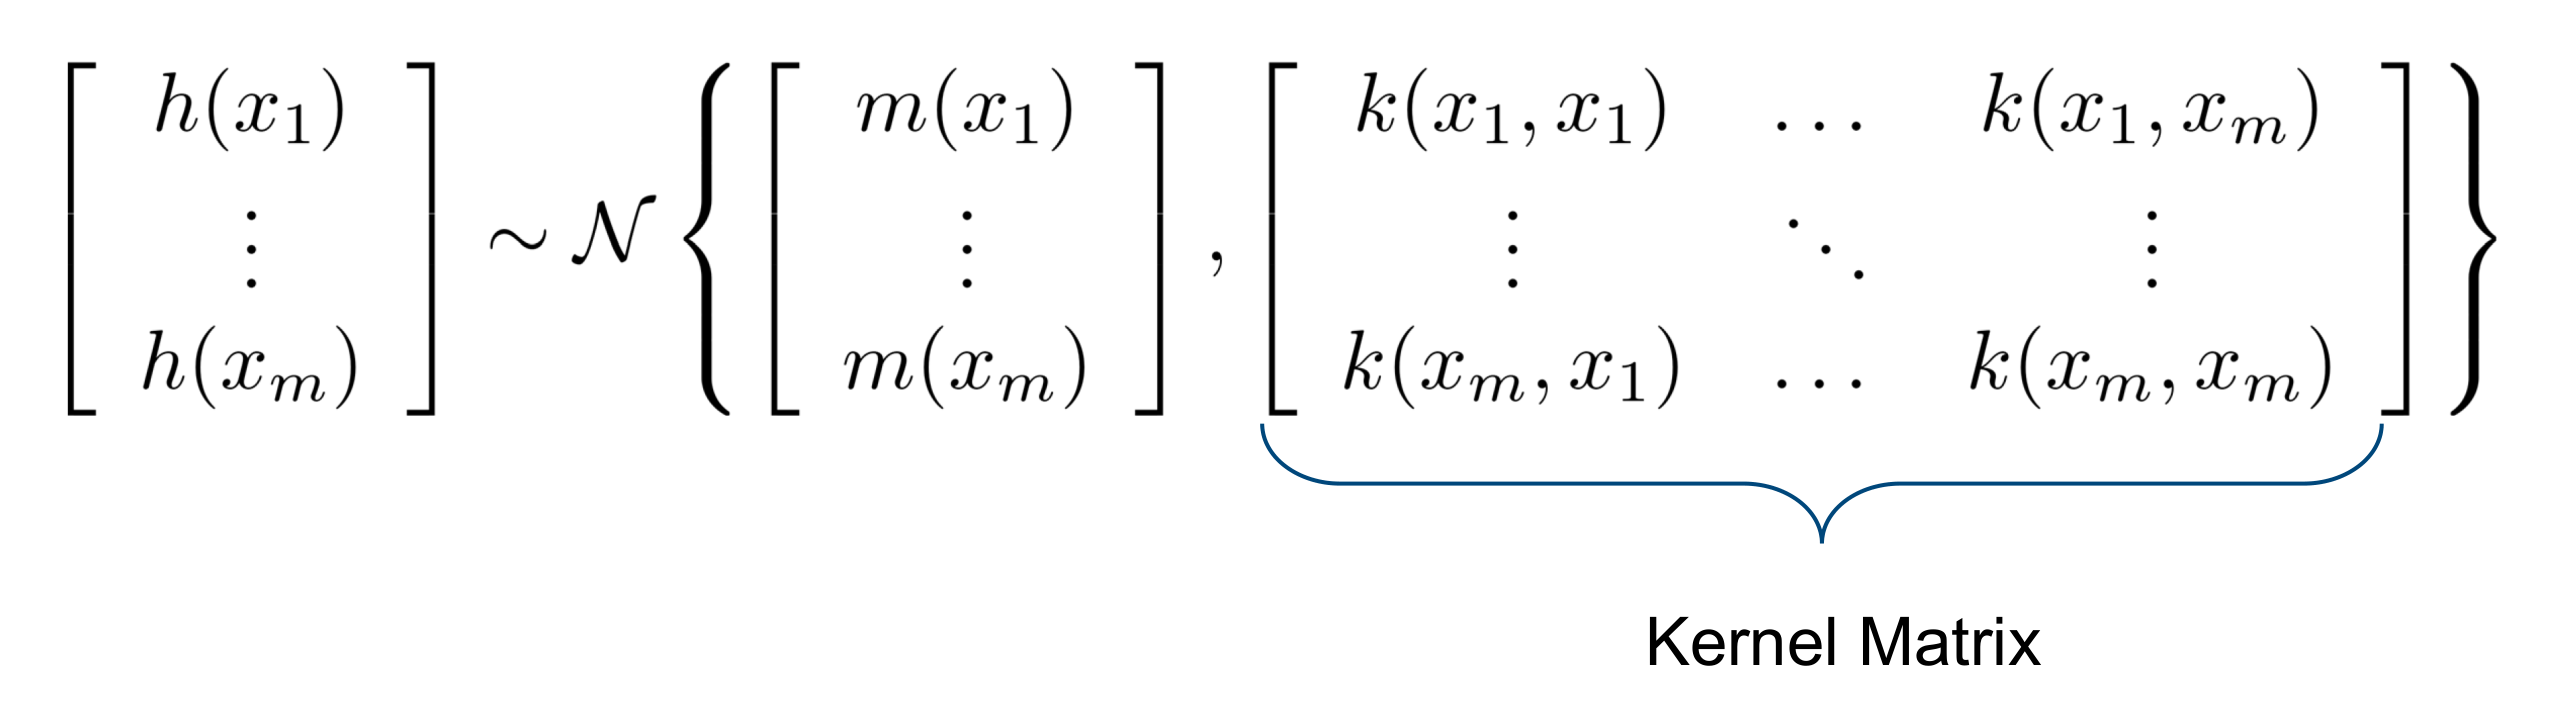
\includegraphics[width=0.8\linewidth]{img/gaussian_processes}
\end{center}

\noindent
\textbf{Gaussian Likelihood}
\begin{align*}
p(\textbf{y}|\textbf{x}, f(x), M_i) &\sim \N{\textbf{f}, \isocov\sigma_n^2}\\
p(\textbf{y}|\textbf{x}, f(x), M_i) &\propto \prod_i e^{-\frac{1}{2\sigma_n^2}\left(y_i -f(x_i)\right)^2}
\end{align*}
With $\isocov$ being the isotropic\footnote{A covariance matrix $\textbf{C}$ is called \emph{isotropic or spherical} if it is proportionate to the identity matrix $\textbf{C} = \lambda\cdot\mathbb{I}$} covariance matrix.

\vspace{1em}
\noindent
Zero mean Gaussian \textbf{process prior}
\begin{equation*}
p(f|M_i) \sim \GP{m(x) \equiv 0, k(x,x')}
\end{equation*}
Gaussian \textbf{process posterior}
\begin{align*}
	p\left( f(x) \middle| \textbf{x},\textbf{y}, M_i \right) &\sim \GP{m_p, k_p(x,x')}\\
	m_p(x) &= k(x,\textbf{x})[K(\textbf{x},\textbf{x}) + \isocov\sigma_n^2]^{-1}\textbf{y}\\
	k_p(x,x') &= k(x,x') - k(x,\textbf{x})[K(\textbf{x},\textbf{x}) + \isocov\sigma_n^2]^{-1} k(\textbf{x},x')
\end{align*}
Gaussian \textbf{predictive distribution}
\begin{align*}
	p\left( y^* \middle| x^*, \textbf{x},\textbf{y}, M_i \right) &\sim \GP{m^*, k^*(x,x')}\\
	m^*(x) &= k(x^*,\textbf{x})[K(\textbf{x},\textbf{x}) + \isocov\sigma_n^2]^{-1}\textbf{y}\\
	k^*(x,x') &= k(x^*,x^*) - k(x^*,\textbf{x})[K(\textbf{x},\textbf{x}) + \isocov\sigma_n^2]^{-1} k(x^*,\textbf{x})
\end{align*}

\subsection{Non-Parametric Gaussian Process Models}
Parametric models assume some finite set of parameters $\theta$. Given the parameters, future predictions $x$, are independent of the observed data $\D$, then $P(x|\theta,\D) = P(x|\theta)$ and therefore $\theta$ captures everything that is to know about the data. This makes the complexity of the model bounded even though the amount of data might be unbounded, and makes the model inflexible. Non-parametric models assume that the data distribution can't be defined in terms of such a finite set of parameters. But they can often be defined by assuming an infinite dimensional $\theta$. Usually $\theta$ is thought of as a function. This gives the following \textbf{Gaussian likelihood}
\begin{equation*}
	p(\textbf{y}| \textbf{x}, f, M_i) \sim \N{\textbf{f}, \isocov\sigma_n^2}
\end{equation*}
And a zero mean Gaussian process prior of
\begin{equation*}
	p(f|M_i) \sim \GP{\textbf{m},\textbf{k}}
\end{equation*}
\textbf{Posterior "functions" distribution} (over functions)
\begin{equation*}
	p(f|\textbf{x},\textbf{y}, M_i) = \frac{p(\textbf{y}| \textbf{x}, f, M_i)\cdot p(f|M_i)}{p(\textbf{y}| \textbf{x},M_i)}
\end{equation*}
Predictive distribution
\begin{equation*}
	p\left( y^* \middle| x^*, \textbf{x},\textbf{y}, M_i \right) = \int p\left( y^* \middle| x^*, f, M_i \right) \cdot p(f|\textbf{x},\textbf{y}, M_i) \diff f
\end{equation*}
Intuitively, one can think of a function $f(\cdot)$ drawn from a Gaussian process prior as an extremely high-dimensional vector drawn from an extremely high- dimensional multivariate Gaussian. In Machine Learning, each dimension of the Gaussian corresponds to an element $x$ from the index set \X, and the corresponding component of the random vector represents the value of $f(x)$.

\subsubsection{Mercer Kernel}
The positive semi-definiteness requirement for covariance matrices computed based on arbitrary input points is identical to \textbf{Mercer's condition for kernels}. A function $(\cdot,\cdot)$ is a valid kernel provided the resulting \textbf{kernel matrix $K$} defined as above is always positive semi-definite for any set of input points $x_1, x_2, \dots, x_m \in \X$. Therefore, Gaussian processes are kernel-based probability distributions in the sense that any valid kernel function can be used as a covariance function.
\begin{definition}
	Let \X be a measure space with $k: L^2(\X\times\X)\rightarrow \R$. $k$ is called a kernel iff there is some feature map $\phi: \X \rightarrow \Hilbert$ into a separable Hilbert space \Hilbert such that
	\begin{equation*}
		k(x,x') = \left\langle \theta(x) \middle| \theta(x') \right\rangle_{\Hilbert}
	\end{equation*}
	that is $k$ is a kernel iff for some space \Hilbert and map $\theta$ the following diagram commutes
	\begin{center}
		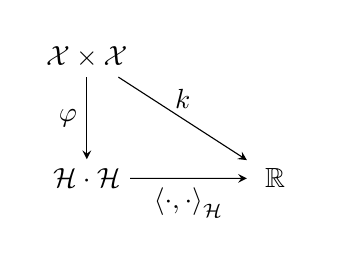
\begin{tikzpicture}
		\matrix (m) [matrix of math nodes,row sep=3em,column sep=4em,minimum width=2em]
		{
			\X\times\X & \\
			\Hilbert\cdot\Hilbert & \R\\
		};
		\path[-stealth]
			(m-1-1) edge node [left] {$\varphi$} (m-2-1)
			edge node [above] {$k$} (m-2-2)
			(m-2-1) edge node [below] {$\left\langle\cdot,\cdot\right\rangle_{\Hilbert}$} (m-2-2);
		\end{tikzpicture}
	\end{center}
	This means that $k(x,x')$ is a kernel, if there is a feature mapping $\varphi(x)$ into some (higher dimensional) space \Hilbert, where it can be represented by a \textbf{scalar or dot product}.
\end{definition}

\subsubsection{Mercer Theorem}
Let \X\ be a measure space with $k:L^2(\X\times\X)\rightarrow \R$ and $k$ be a function with the following properties
\begin{itemize}
	\item $k$ is \emph{symmetric}:
	\begin{equation*}
		k(x,x') = k(x',x)
	\end{equation*}
	\item $k$ is \emph{positive-semidefinite}:
	\begin{equation*}
		k(x,x') \geq\qquad \forall x,x'
	\end{equation*}
	\item $k$ is \emph{continuous}: $k(x,x') \rightarrow \R$ is a continuous function in $x$ and $x' \in \X$ 
\end{itemize}
Then there is a feature mapping $\theta : \X \rightarrow \R^d$, such that
\begin{equation*}
	k(x,x') = \left\langle \theta(x) \middle| \theta(x') \right\rangle_\Hilbert = \theta(x)^T \cdot \theta(x')
\end{equation*}

\subsubsection{Kernel Properties}
If $k_1(x,y)$ and $k_1(x,y)$ are kernels, then the following functions are kernels as well
\begin{align*}
	k(x,y) &= \langle\theta(x) | \theta(x')\rangle_{\mathcal{F}}\\
	k(x,y) &= k_1(x,y) + k_2(x,y)\\
	k(x,y) &= \alpha\cdot k_1(x,y)\qquad\text{where}\ \alpha>0\\
	k(x,y) &= f(x) \cdot f(y)\qquad\text{for any function}\ f(x)\\
	k(x,y) &= k_1(x,y) \cdot k_2(x,y)
\end{align*}

\subsubsection{Radial Basis Function or Squared Exponential Kernel}
\begin{equation*}
	k(x,x') = \sigma_0^2 e^{-\frac{1}{2}\left(\frac{x-x'}{\lambda}\right)^2}
\end{equation*}
The radial basis function kernel (RBF) kernel is a stationary kernel. It is known as the \textbf{squared exponential kernel} as well and parametrised by a length-scale parameter $\lambda$. This parameter can either be a scalar (the isotropic variant of the kernel) or a vector with the same number of dimensions as the inputs (the anisotropic variant of the kernel). The RBF kernel is infinitely differentiable, which implies that a $\mathcal{GP}$ with this kernel as covariance function has mean square derivatives of all orders, and \textbf{is thus very smooth}.

\subsubsection{Rational-Quadratic Kernel}
\begin{equation*}
	k(x,x') = \left( 1 + \frac{(x-x')^2}{2\alpha\lambda^2} \right)^{-\alpha}
\end{equation*}

\noindent
\begin{minipage}{0.55\linewidth}
	The Rational Quadratic kernel can be seen as a scale mixture (an infinite sum) of RBF kernels with different characteristic length-scales. It is parametrised by a length-scale parameter $\lambda$ and a scale mixture parameter $\alpha$.
\end{minipage}
\hfill
\begin{minipage}{0.42\linewidth}
	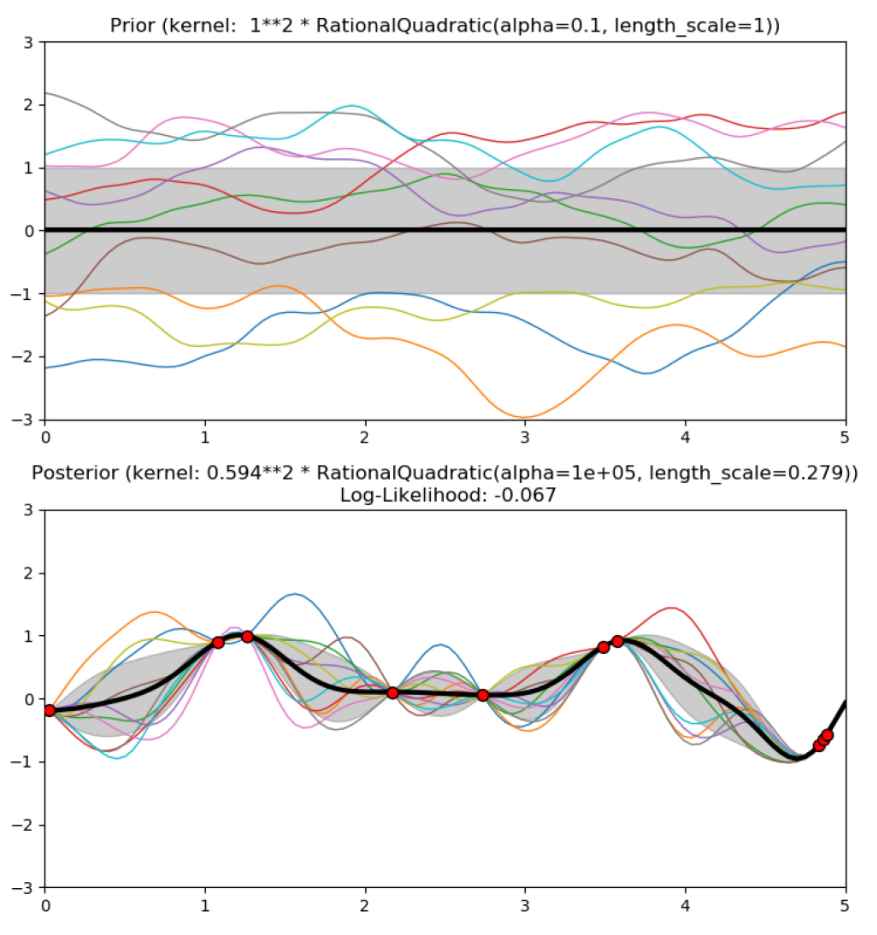
\includegraphics[width=\linewidth]{img/rational_quadratic_kernel}
\end{minipage}

\subsubsection{Exp-Sine-Squared Kernel}
\begin{equation*}
	k(x,x') = e^{-\frac{2\cdot \sin^2\left(\frac{\pi}{p}\cdot\abs{x-x'}\right)}{\lambda^2}}
\end{equation*}

\noindent
\begin{minipage}{0.55\linewidth}
	The Exp-Sine-Squared kernel allows modelling periodic functions. An example of such a periodic function would be the $\text{CO}_2$ concentration or daily temperature changes. It is parametrised by a length-scale parameter $\lambda$ and a periodicity parameter $p$.
\end{minipage}
\hfill
\begin{minipage}{0.42\linewidth}
	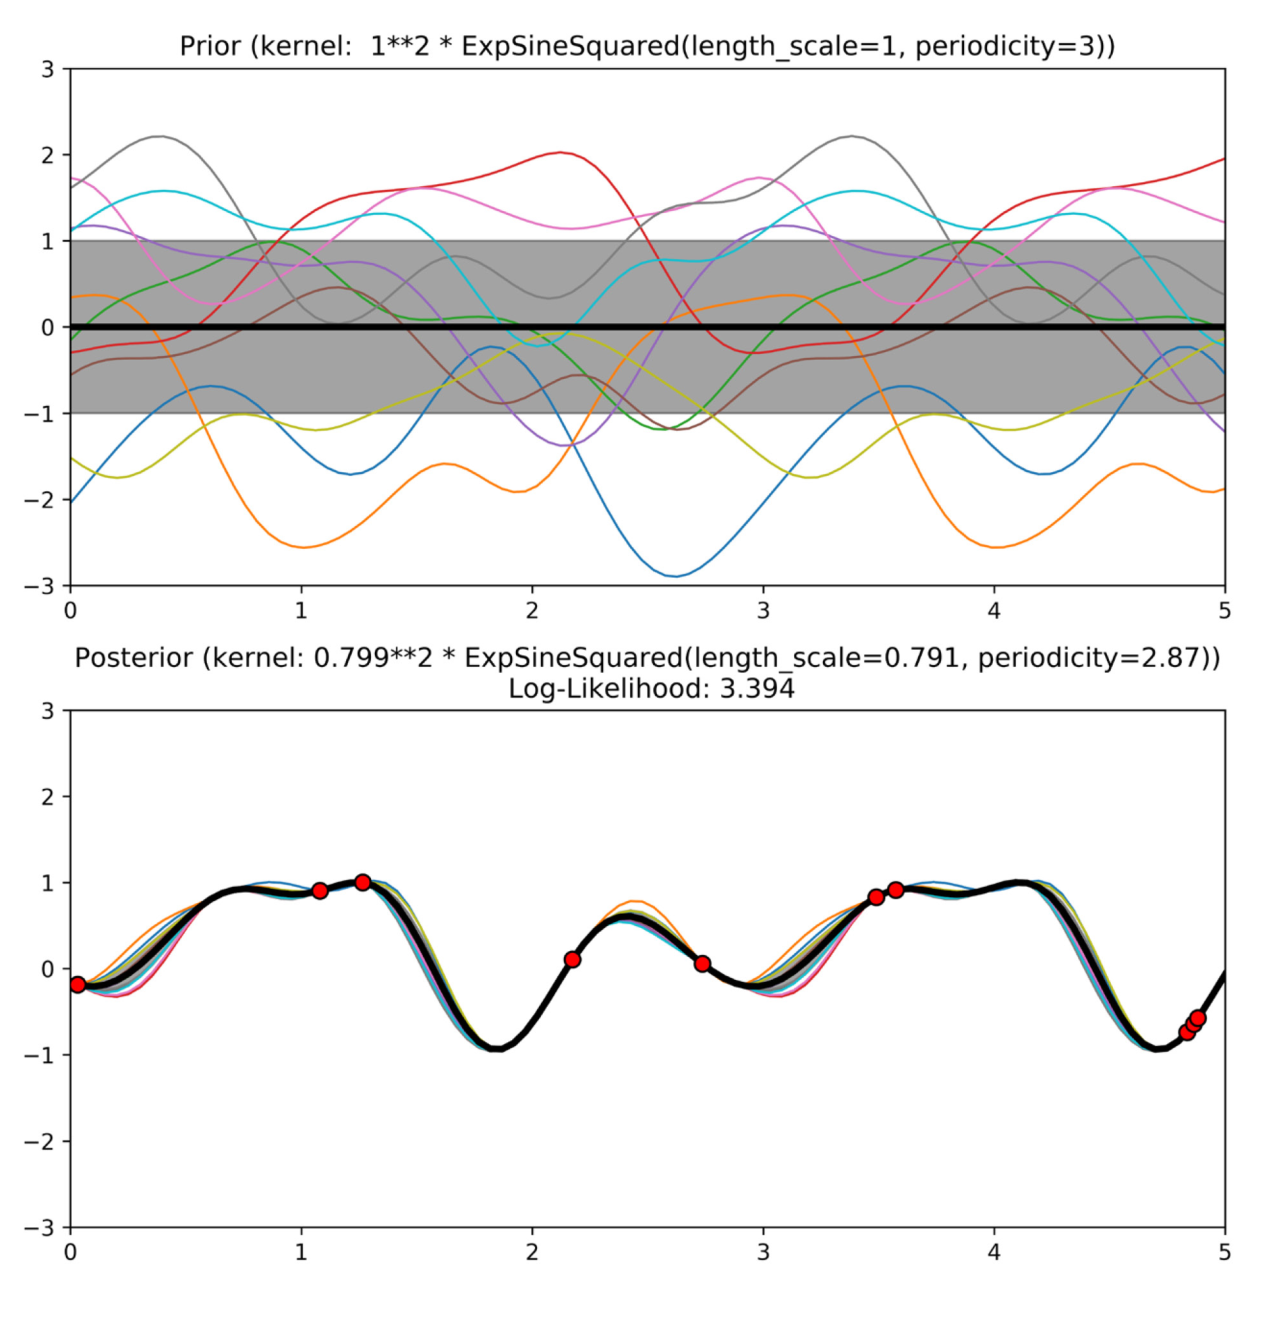
\includegraphics[width=\linewidth]{img/exp_sine_kernel}
\end{minipage}

\subsubsection{Dot-Product Kernel}
\begin{equation*}
	k(x,x') = \sigma_0^2 + x\cdot x'
\end{equation*}

\noindent
\begin{minipage}{0.55\linewidth}
	The Dot-Product kernel is non-stationary and can be obtained from linear regression by putting $a_d \sim \N{0,1}$ priors on the coefficients of $x_d\quad d=1..D$ and a prior of $b_0 \sim \N{0,\sigma_0^2}$ on the bias. The Dot-Product kernel is invariant to a rotation of the coordinates about the origin, but not translations. It is parametrised by a parameter $\sigma_0^2$. For $\sigma_0^2=0$ the kernel is called the homogeneous linear kernel, otherwise it is inhomogeneous.
\end{minipage}
\hfill
\begin{minipage}{0.42\linewidth}
	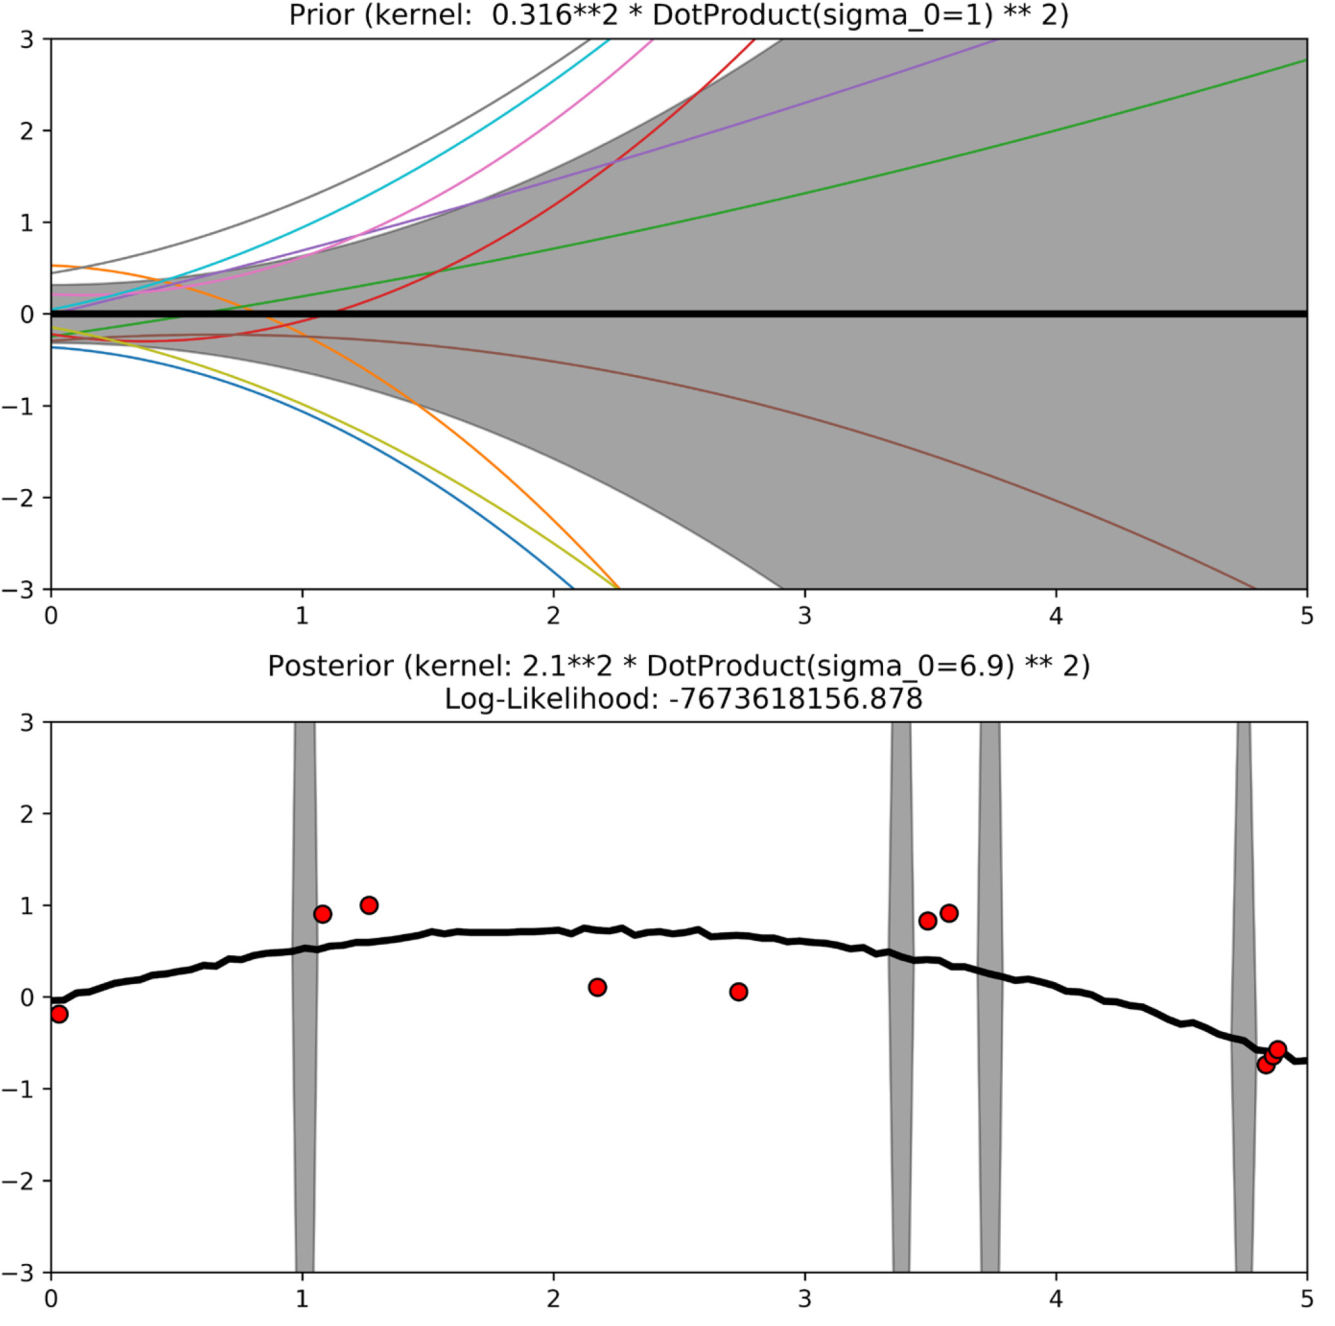
\includegraphics[width=\linewidth]{img/dot_product_kernel}
\end{minipage}

\subsubsection{Matérn Kernel}
\begin{equation*}
	k(x_i, x_j) =  \frac{1}{\Gamma(\nu)2^{\nu-1}}\left( \frac{\sqrt{2\nu}}{l} d(x_i , x_j ) \right)^\nu K_\nu\left( \frac{\sqrt{2\nu}}{l} d(x_i , x_j )\right)
\end{equation*}

\noindent
\begin{minipage}{0.55\linewidth}
	The Matérn kernel is a stationary kernel and a generalization of the RBF kernel. It has an additional parameter $\nu$ which controls the smoothness of the resulting function. It is parametrised by a length-scale parameter $\lambda$, which can either be a scalar (isotropic variant of the kernel) or a vector with the same number of dimensions as the inputs (anisotropic variant of the kernel). 
	
	For a finite $\nu$, the Matérn kernel generates much rougher sample functions than RBF. For the special case of $\nu = \frac{1}{2}$ the kernel becomes $ k(x,x') = e^{-\abs{x-x'}\lambda}$. This is called an \textbf{Ornstein-Uhlenbeck process}, yielding very rough sample functions.
\end{minipage}
\hfill
\begin{minipage}{0.42\linewidth}
		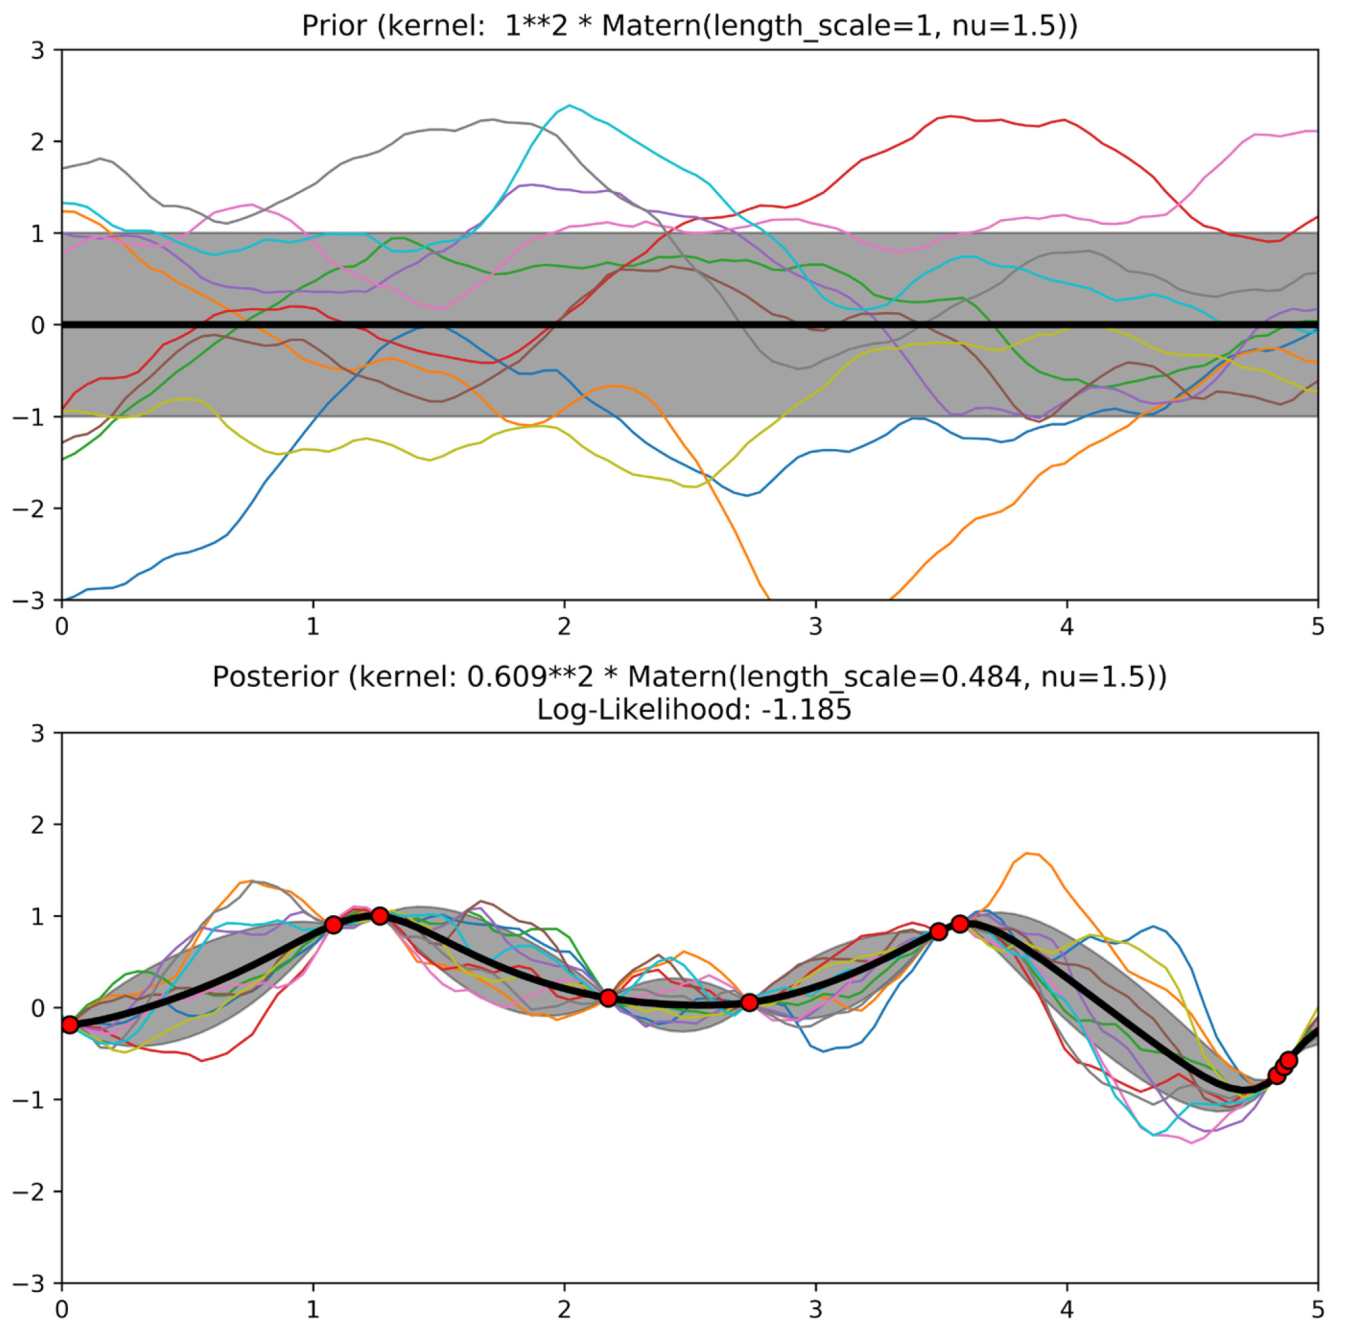
\includegraphics[width=\linewidth]{img/matern_kernel}
\end{minipage}

\subsection{Section Summary}
\begin{itemize}
	\item \emph{Assumptions} are made explicit in the form of a \textbf{prior}
	\item \emph{Predictions} are made by \textbf{averaging over the posterior}, taking all possible interpretations of the data into account
	\item Bayesian inference does not involve any maximization so there is \textbf{no possibility of over-fitting}. Instead, parameters are integrated out.
	\item Bayesian inference is \textbf{usually difficult}, because it is difficult to do integrals.
\end{itemize}

\section{Dimensionality Reduction}
The "Curse of Dimensionality" is the problem that inputs are high dimensional when working with data from speech, images, genomes and other sources. One of the characteristics of high-dimensional data is that the number of dimensions is comparable or larger than the number of samples. This has the consequence that the sample complexity of function approximation can grow exponentially.

\begin{figure}[H]
	\centering
	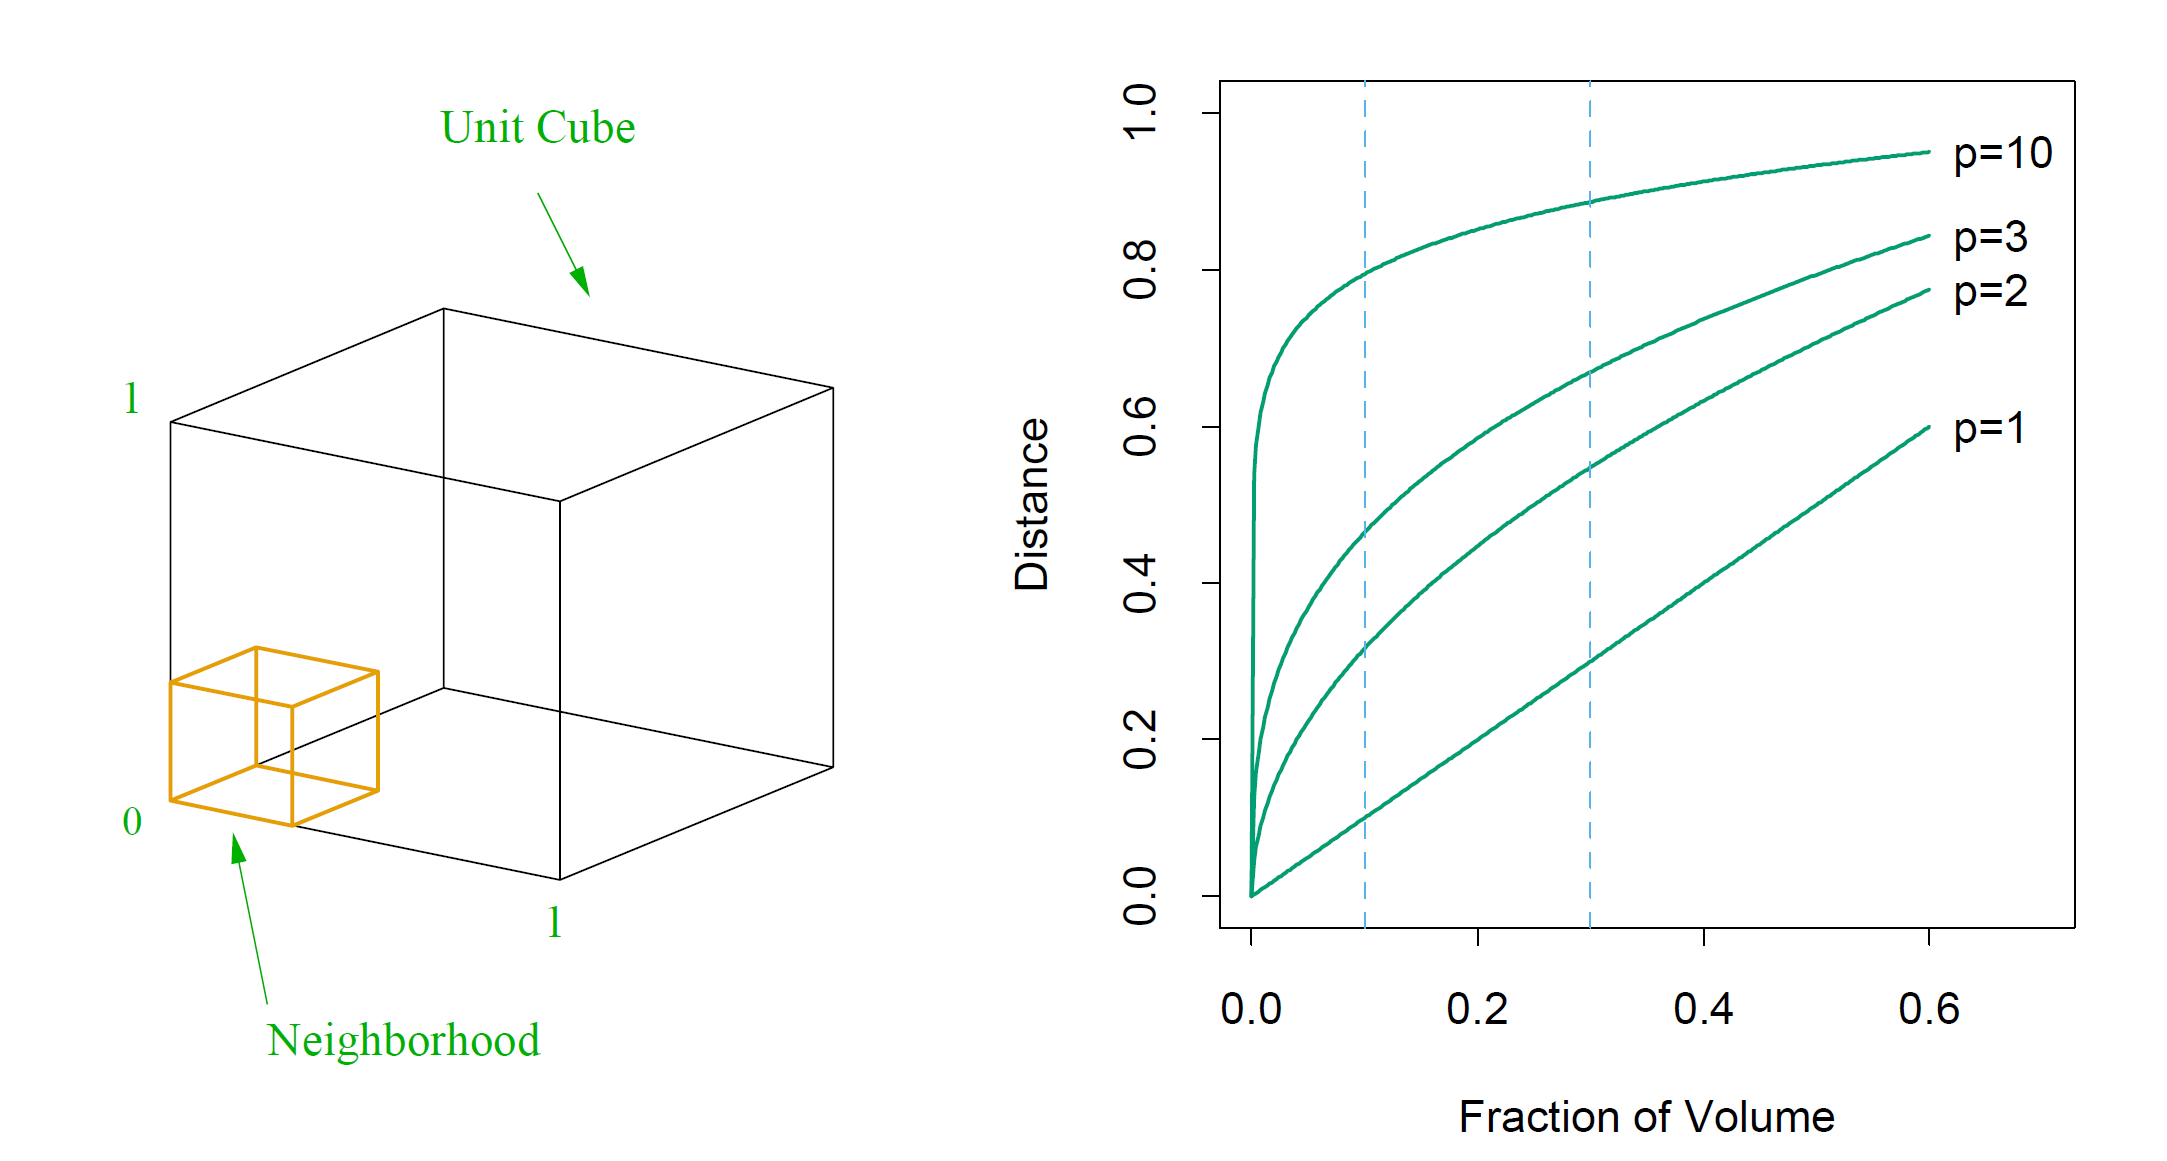
\includegraphics[width=0.6\linewidth]{img/curse_dimensionality}
	\caption{The curse of dimensionality is well illustrated by a sub-cubical neighbourhood for uniform data in a unit cube. The figure on the right shows the side-length of the sub-cube needed to capture a fraction r of the volume of the data, for different dimensions p. In ten dimensions we need to cover 80\% of the range of each coordinate to capture 10\% of the data.}
	\label{fig:cursedimensionality}
\end{figure}

High dimensional data is very sparse: most training instances are likely to be far away from each other making predictions much harder, greater risk of overfitting, joint probabilities are hard to fit.

\subsection{Dimensionality Reduction}
Dimensionality reduction is the process of reducing the number of random variables under consideration by obtaining a set of principal variables.
\begin{itemize}
	\item \textbf{Feature Reduction} approaches try to find a subset of the original variables (also called features or attributes).
	\begin{itemize}
		\item filter strategy, \emph{information gain}
		\item wrapper strategy, \emph{search guided by accuracy}
		\item embedded strategy, \emph{features are selected to add or be removed while building the model based on the prediction errors}
	\end{itemize}
	\item \textbf{Feature Extraction} transforms the data in the high-dimensional space to a space of fewer dimensions
\end{itemize}

\newpage
\noindent
\begin{tabularx}{\linewidth}{m{0.2\linewidth} m{0.6\linewidth}}
	\multicolumn{2}{l}{\textbf{Linear Techniques}}\\
	\hline
	&\\[-0.5em]
	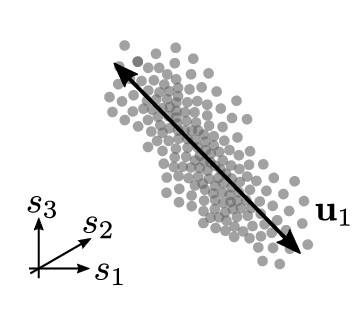
\includegraphics[width=\linewidth]{img/input_data_variance} & Several methods (starting from PCA) attempt to identify the low- dimensional subspace that captures the largest fraction of the input data variance\\
	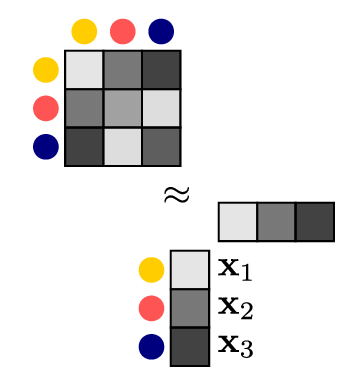
\includegraphics[width=\linewidth]{img/kernel_method} & This is equivalent to finding the best L2-norm approximation of the Gram matrix, and generalises to \textbf{kernel methods}\\
	& \\
	\multicolumn{2}{l}{\textbf{Manifold Techniques}}\\
	\hline
	&\\[-0.5em]
	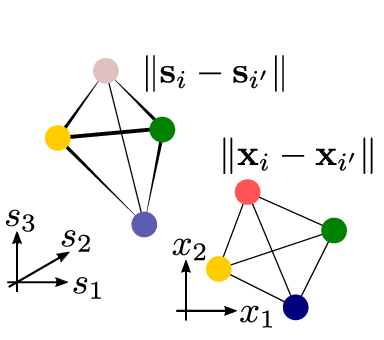
\includegraphics[width=\linewidth]{img/multi-dimensional_scaling} & \textbf{Multi-dimensional scaling} and related approaches attempt to reproduce the similarity between high-dimensional data points in low dimension\\
	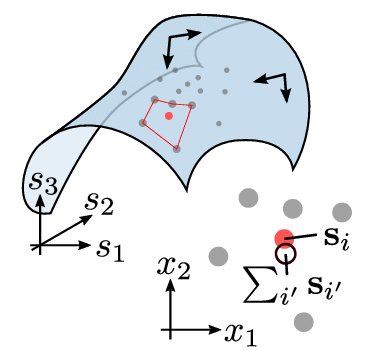
\includegraphics[width=\linewidth]{img/embedding_methods} & \textbf{Embedding methods} explicitly try to preserve local relations between points, under the assumption that they lie on a (locally) low-dimensional manifold
\end{tabularx}

\subsection{Principal Component Analysis}
The main linear technique for dimensionality reduction, principal component analysis PCA, performs a linear mapping of the data to a lower-dimensional space in such a way that the variance of the data in the low-dimensional representation is maximized.

The eigenvectors that correspond to the largest eigenvalues (the principal components) can now be used to reconstruct a large fraction of the variance of the original data. PCA identifies the d-dimensional hyperplane that lies closest to the data and then projects the data on it (d is a hyperparameter).

\begin{center}
	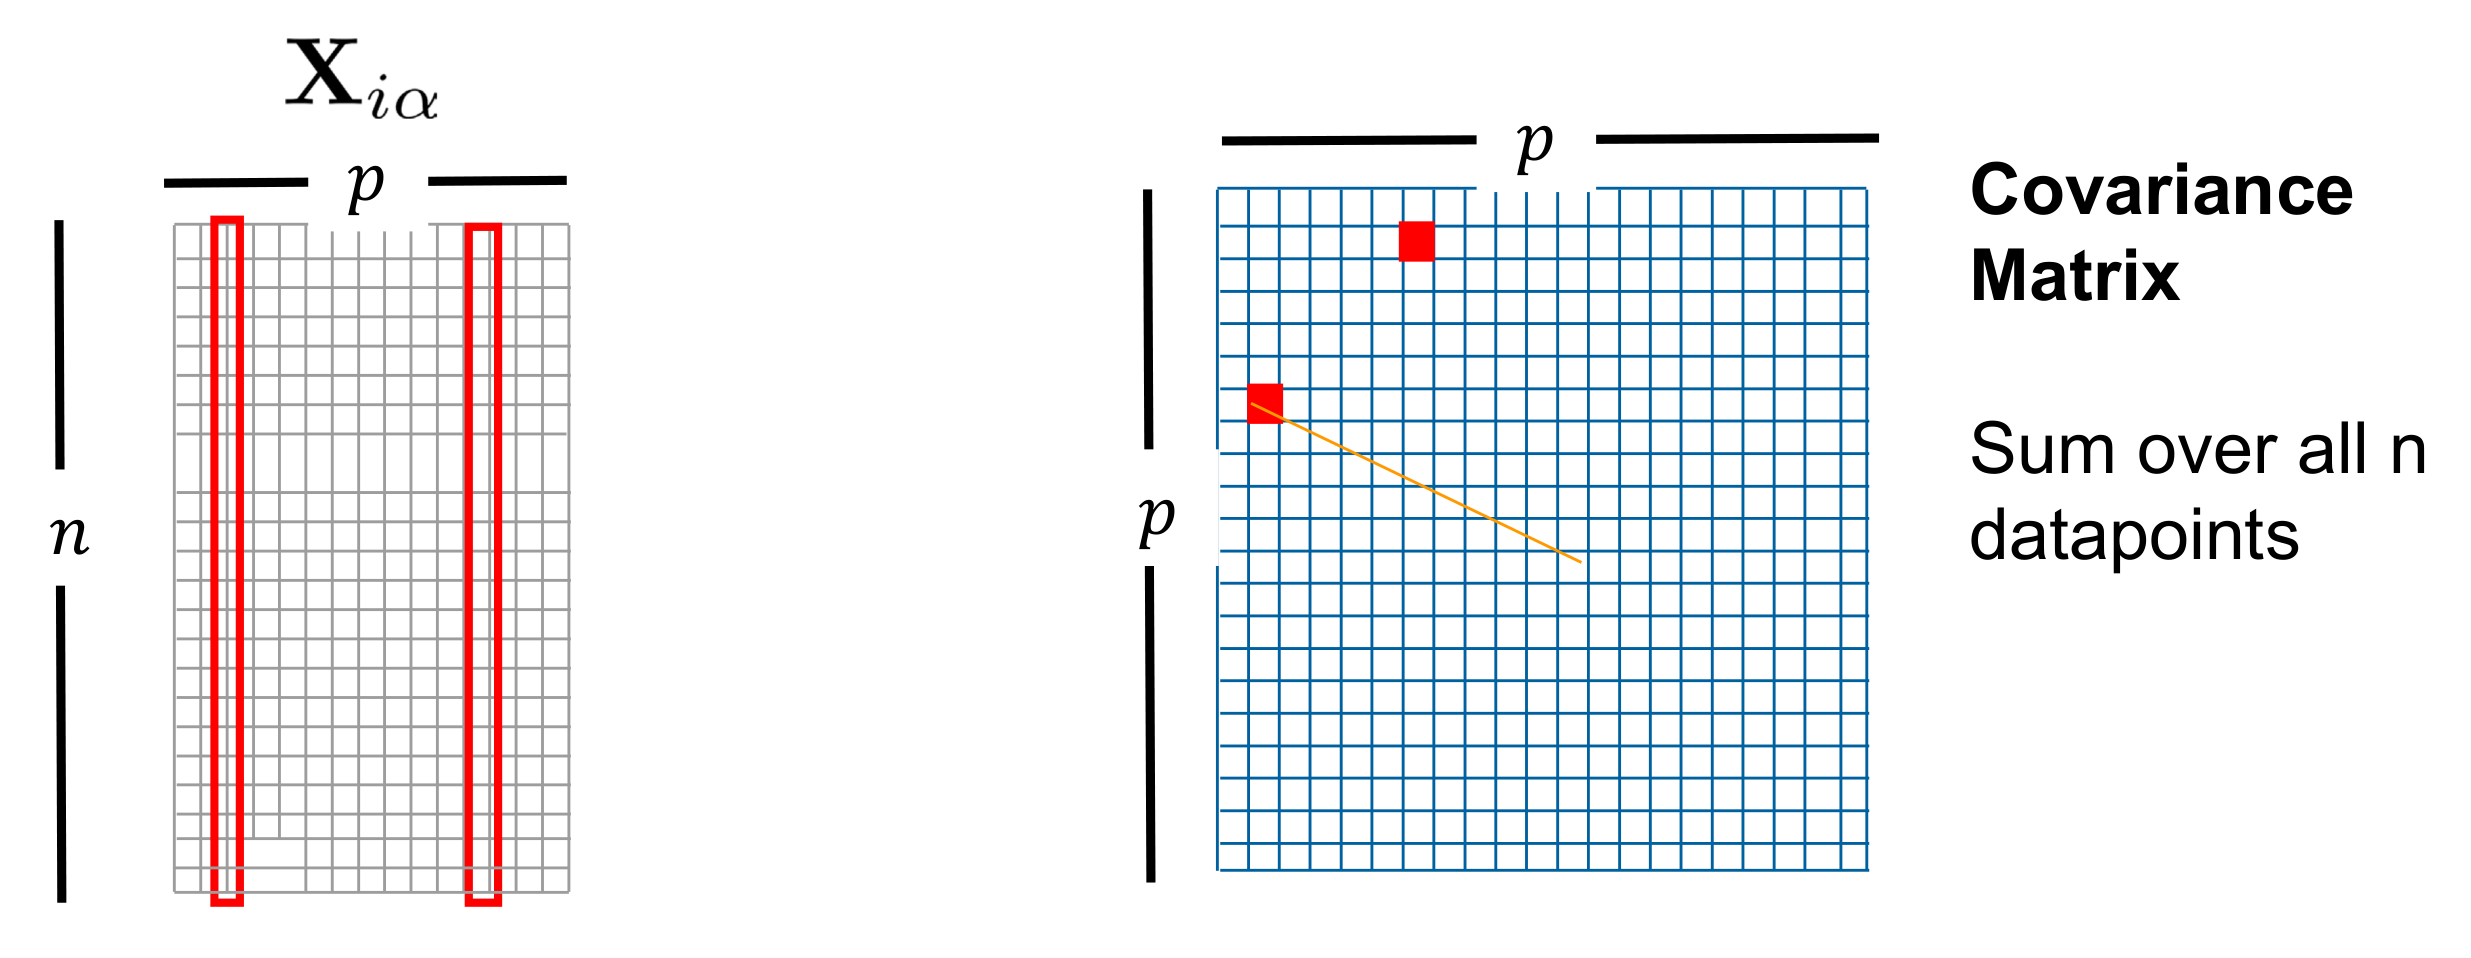
\includegraphics[width=0.7\linewidth]{img/input_covariance_matrix}
\end{center}

\begin{align*}
	\textbf{C}_ij &= \left\langle (\textbf{X}_i - \left\langle \textbf{X}_i \right\rangle) (\textbf{X}_j - \left\langle \textbf{X}_j \right\rangle) \right\rangle\\
	\left\langle \textbf{X}_i \right\rangle &= 0 \Rightarrow \textbf{C} = \textbf{X}^T \textbf{X}
\end{align*}
It turns out that the optimization corresponds to a diagonalization of the covariance matrix $  \textbf{C} = \textbf{U}\textbf{D}\textbf{U}^T$. PCA is a rotation or reflection so that the first principal component has the highest variance, the second is orthogonal to the first and has the second highest variance and so forth. $\textbf{X}$ is the $n\times p$-dimensional data matrix column centred.
\begin{center}
	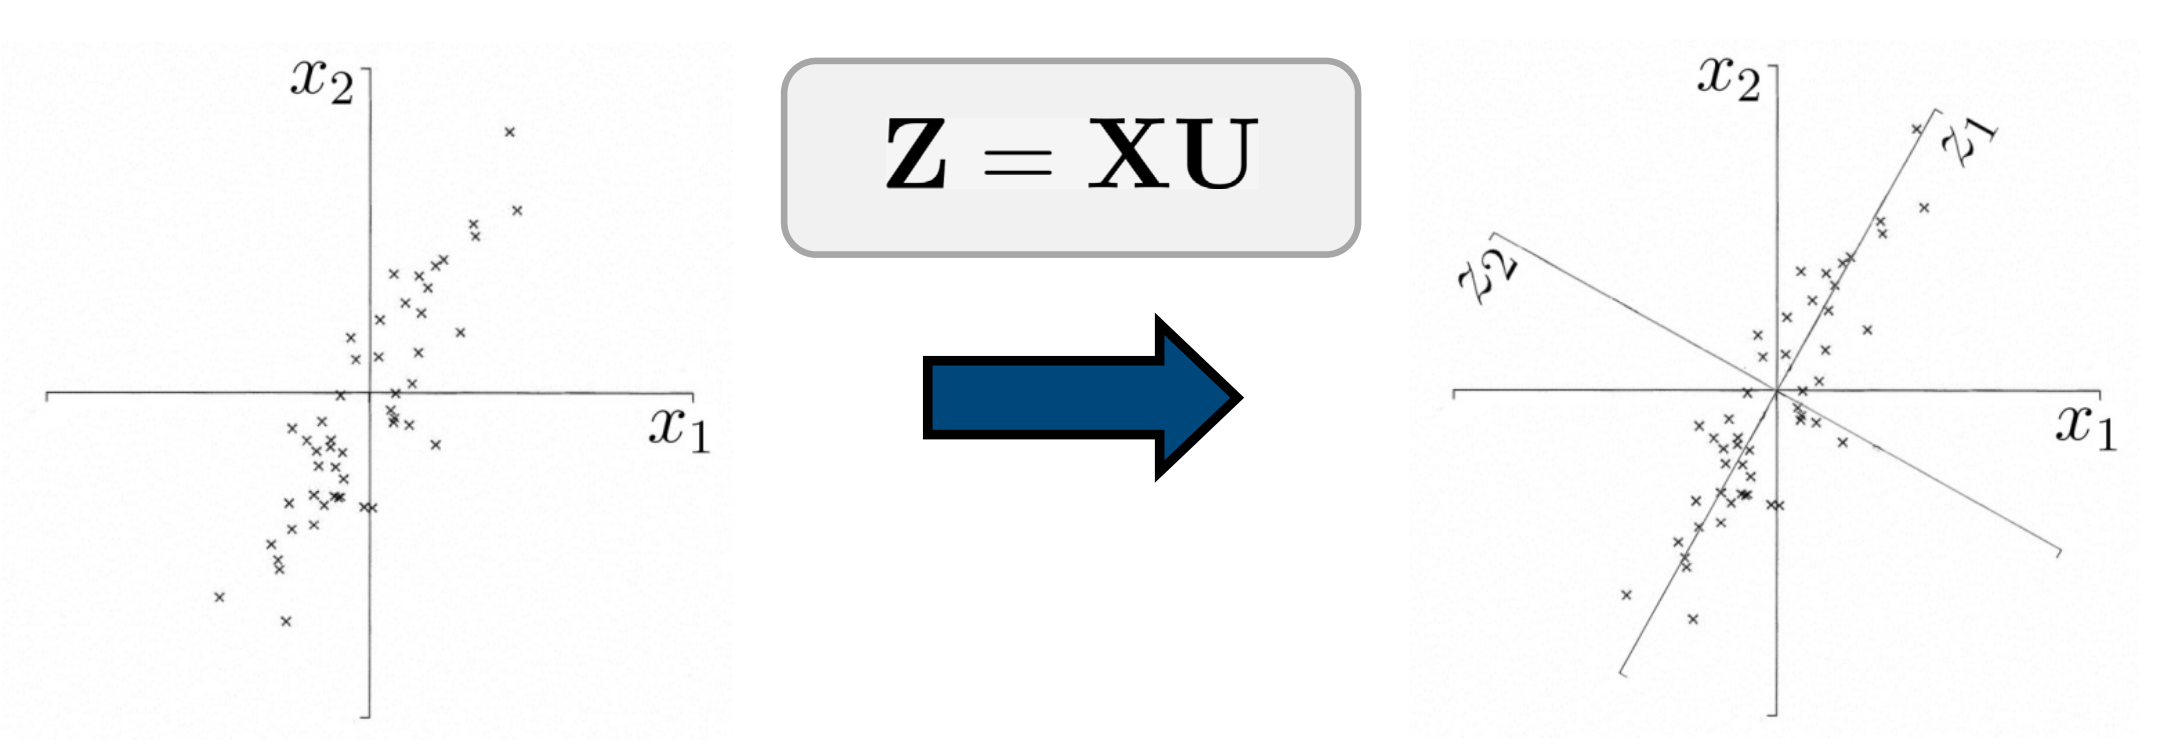
\includegraphics[width=0.7\linewidth]{img/PCA_X}
\end{center}

\subsubsection{Explained Variance Ratio $P_k$}
\begin{minipage}{0.55\linewidth}
	The percentage the first $k$ dimensions contribute to the variance.
	\begin{equation*}
	P_k = \frac{\sum_{i=1}^k \text{var}\left(\textbf{X}_i\right)}{\sum_{j=1}^p \text{var}\left(\textbf{X}_j\right)} = \frac{\sum_{i=1}^{k} \lambda_i}{\sum_{j=1}^{p} \lambda_j}
	\end{equation*}
\end{minipage}
\begin{minipage}{0.4\linewidth}
	\begin{center}
		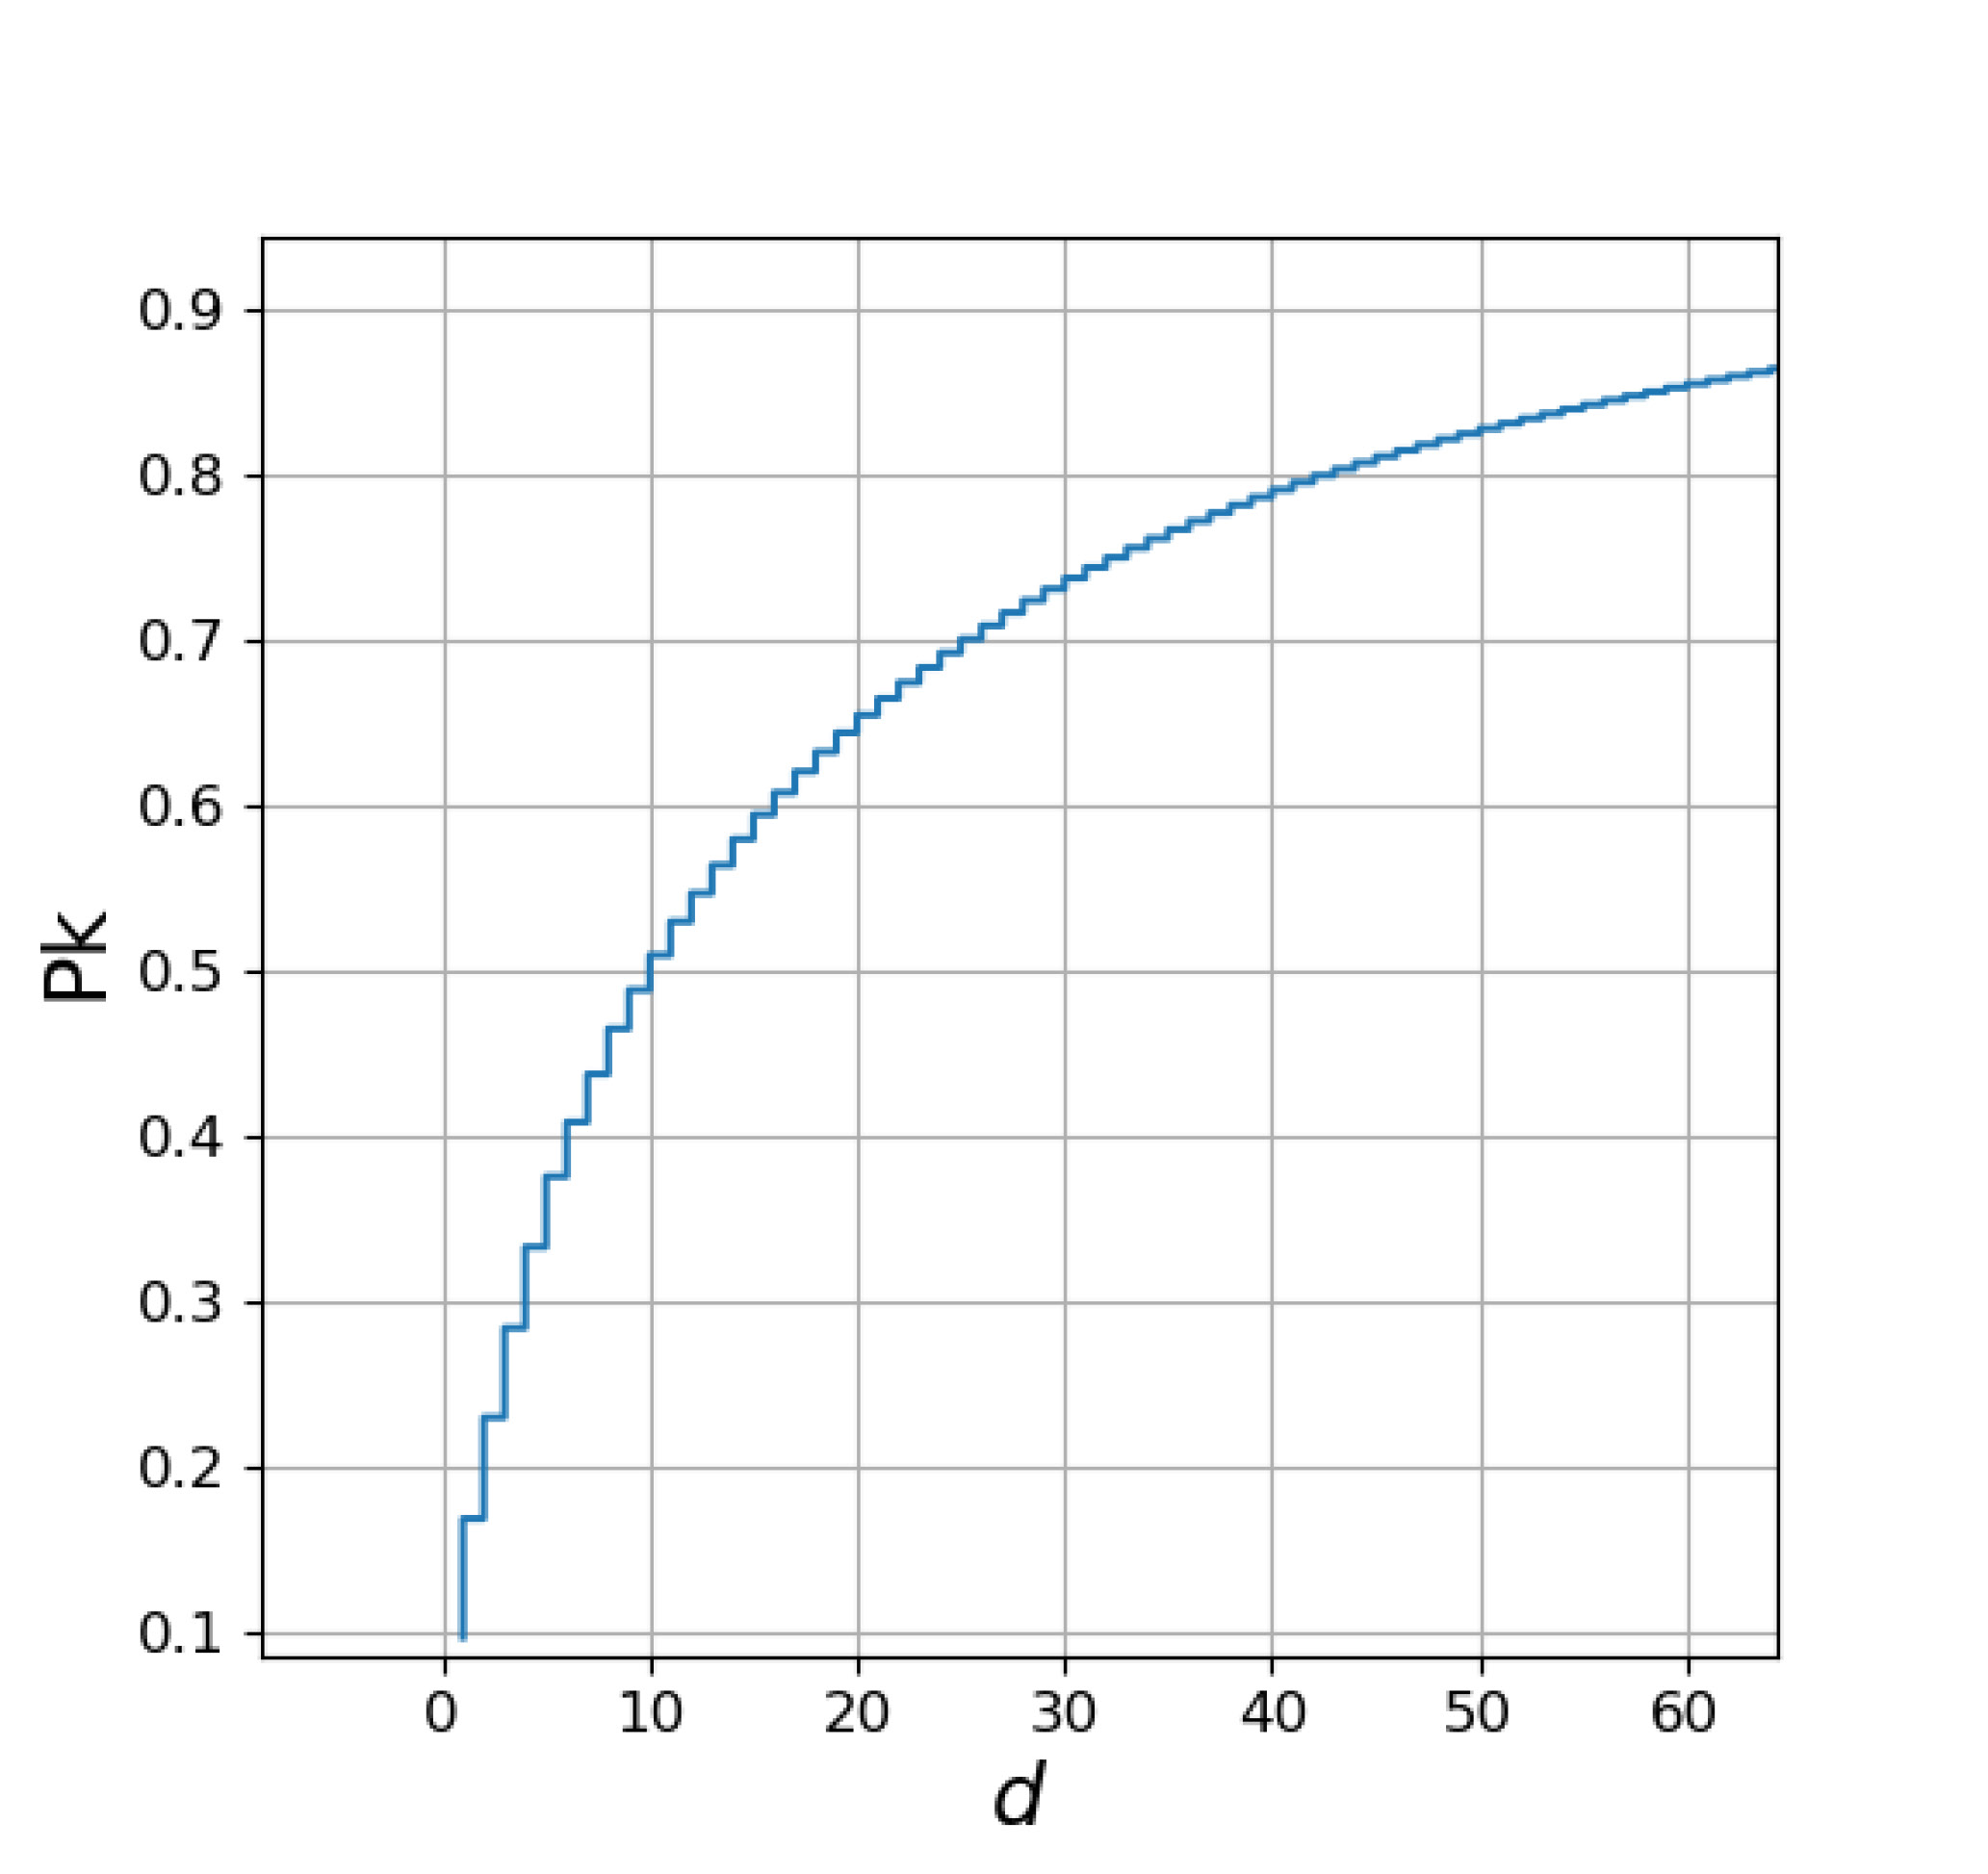
\includegraphics[width=\linewidth]{img/explained_variance_ratio}
	\end{center}
\end{minipage}

\begin{minted}{python}
pca = PCA(n_components=0.80)
pca.explained_variance_ratio_
1 - pca.explained_variance_ratio_.sum
\end{minted}

\subsubsection{Choosing The Right $k$}
The first criterion, the total variance $V_{tot}$, can be calculated as (total variance is preserved under rotation)
\begin{equation*}
	V_{tot} = \sum_{j=1}^{p}\Var{\textbf{X}_j} = \sum_{j=1}^{p} \Var{\textbf{Z}_j} = \sum_{j=1}^{p} \lambda_j
\end{equation*}
While the second criterion, $P_k$ as a function of the dimension, can only be obtained through testing (grid search)
\begin{center}
	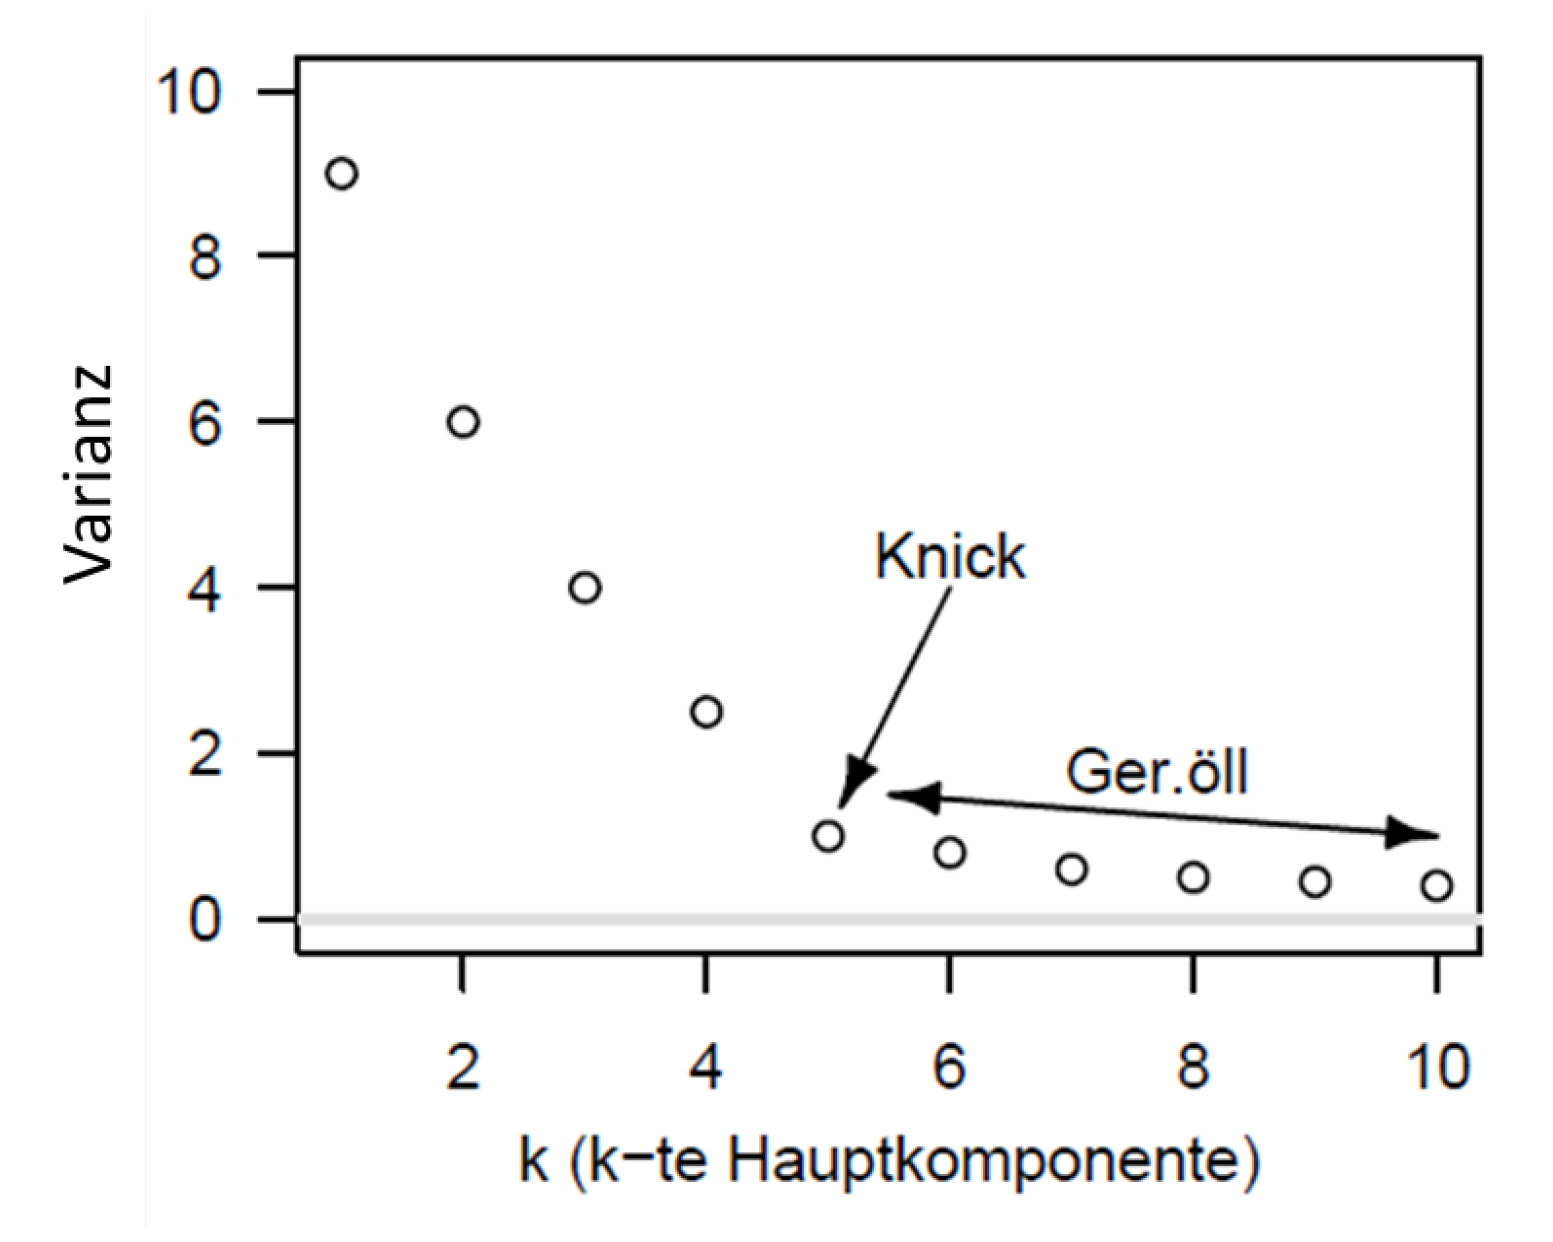
\includegraphics[width=0.4\linewidth]{img/pca_k}
\end{center}

\subsection{Maximum Variance Formulation}
Given $D$-dimensional data vectors $\{\textbf{x}_n\}\ (n=1..N)$ and a data matrix $X_{(D\times N)} = \left[\textbf{x}_1,\dots, \textbf{x}_N\right]$, project the data to an $M$-dimensional subspace with $M<D$ while maximising the variance of the projected data.

Assuming $M=1$, then there is a $D$-dimensional vector $\textbf{u}_1$ that does this. As only the direction defined by this vector and not the magnitude of $\textbf{u}_1$ itself is interesting, the norm is to choose a unit vector so that $\textbf{u}_1^T\textbf{u}_1 = 1$.

The mean $\overline{\textbf{x}}_p$ and variance $\text{Var}_p$ of the projected data are given by
\begin{tabularx}{\linewidth}{m{0.3\linewidth} m{0.7\linewidth}}
	projected data & \[ \samplemean{\textbf{x}}_p = \textbf{u}_1^T\samplemean{\textbf{x}} \]\\
	data mean & \[ \samplemean{\textbf{x}} = \frac{1}{N}\sum_{n=1}^{N}\textbf{x}_n \]\\
	variance of projected data & \[\text{Var}_p = \frac{1}{N}\sum_{n=1}^{N}\{\textbf{u}_1^T\textbf{x}_n - \textbf{u}_1^T\samplemean{\textbf{x}}\}^2 = \textbf{u}_1^T C \textbf{u}_1 \]\\
	data covariance matrix & \[ C = \frac{1}{N}\sum_{n=1}^{N}(\textbf{x}_n - \samplemean{\textbf{x}})(\textbf{x}_n - \samplemean{\textbf{x}})^T \]
\end{tabularx}
\noindent
Maximise $\text{Var}_p$ under the constraint, that the norm of the projection operator is one ($\textbf{u}_1^T\textbf{u}_1 = 1$). Use a Lagrange multiplier $\lambda_1$ to be able to use unconstrained optimisation
\begin{align*}
	 L(\textbf{u}_1, \lambda_1) &= \textbf{u}_1^T C \textbf{u}_1 + \lambda_1(1 - \textbf{u}_1^T\textbf{u}_1) \tag*{\textbf{Lagrange Function}}\\
	\left.\begin{matrix}\frac{\partial L}{\partial \textbf{u}_1} = 0\\ \frac{\partial L}{\partial \lambda_1} = 0\end{matrix}\right\} &\Rightarrow \textbf{u}_1 = \lambda_1\textbf{u}_1\\
	&\Rightarrow \textbf{u}_1^T C \textbf{u}_1 = \lambda_1
\end{align*}
The variance will be a maximum when $\textbf{u}_1$ is set equal to the eigenvector of $C$ having the largest eigenvalue $\lambda_1$. This eigenvector is known as the \textbf{first principal component}.

Additional principal components $\lambda_k$ can be defined in an incremental fashion by choosing each new direction that maximises the variance amongst all possible directions orthogonal to those already considered. The optimal linear projection matrix is then given by $[\textbf{u}_1,\textbf{u}_2,\dots,\textbf{u}_M]$ \parencite[p. 561-565]{bishop2006pattern}.

\subsection{Kernel PCA}
Principal component analysis can be employed in a nonlinear way by means of the kernel trick. Data that inseparable in the input space can be transformed in higher dimensional space where it is linearly separable. For example
\begin{equation*}
	\theta: \R^2 \rightarrow \R^2 : (x_1,x_2) \mapsto (x_1,x_2, x_1^2 + x_2^2)
\end{equation*}
High-dimensional mapping can seriously increase computation time. But by using the \textbf{Kernel-Trick} this can be avoided
\begin{equation*}
	K(x_i,x_j) = \theta(x_i)^T\cdot \theta(x_j)
\end{equation*}
Given any algorithm that can be expressed solely in terms of \textbf{dot products}, this trick allows us to \textbf{construct different non-linear versions} of it.

\subsubsection{Popular Kernels}
\begin{tabularx}{\linewidth}{m{0.3\linewidth} m{0.7\linewidth}}
	Gaussian (RBF) & \[ K(\textbf{x},\textbf{x}') = e^{-\beta\cdot\norm{\textbf{x}-\textbf{x}'}^2} \]\\
	Laplacian & \[ K(\textbf{x},\textbf{x}') = e^{-\gamma\abs{\textbf{x}-\textbf{x}'}_1} \]\\
	Polynomial & \[ K(\textbf{x},\textbf{x}') = (1+\textbf{x}^T\textbf{x}')^p \]\\
	Sigmoid & \[ K(\textbf{x},\textbf{x}') = \tanh(\alpha \textbf{x}^T\textbf{x}' + \delta) \]\\
	Linear Kernel & \[ K(\textbf{x},\textbf{x}') = \textbf{x}^T\textbf{x}' \]\\
\end{tabularx}
\noindent
Kernel Principal Component Analysis (KPCA) extends conventional principal component analysis (PCA) to a high dimensional feature space $D$ using the \textbf{kernel trick}.
\begin{enumerate}
	\item Mapping to a non-linear feature space\quad$x_i\mapsto\theta(x_i)$
	\item Extract the PCA in that space, the result will be non-linear in the original space
\end{enumerate}

\subsection{Manifold Learning}
A collection of methodologies for analyzing high dimensional data based on the hypothesis that data tend to lie near a low dimensional manifold is now called Manifold Learning.

\begin{center}
	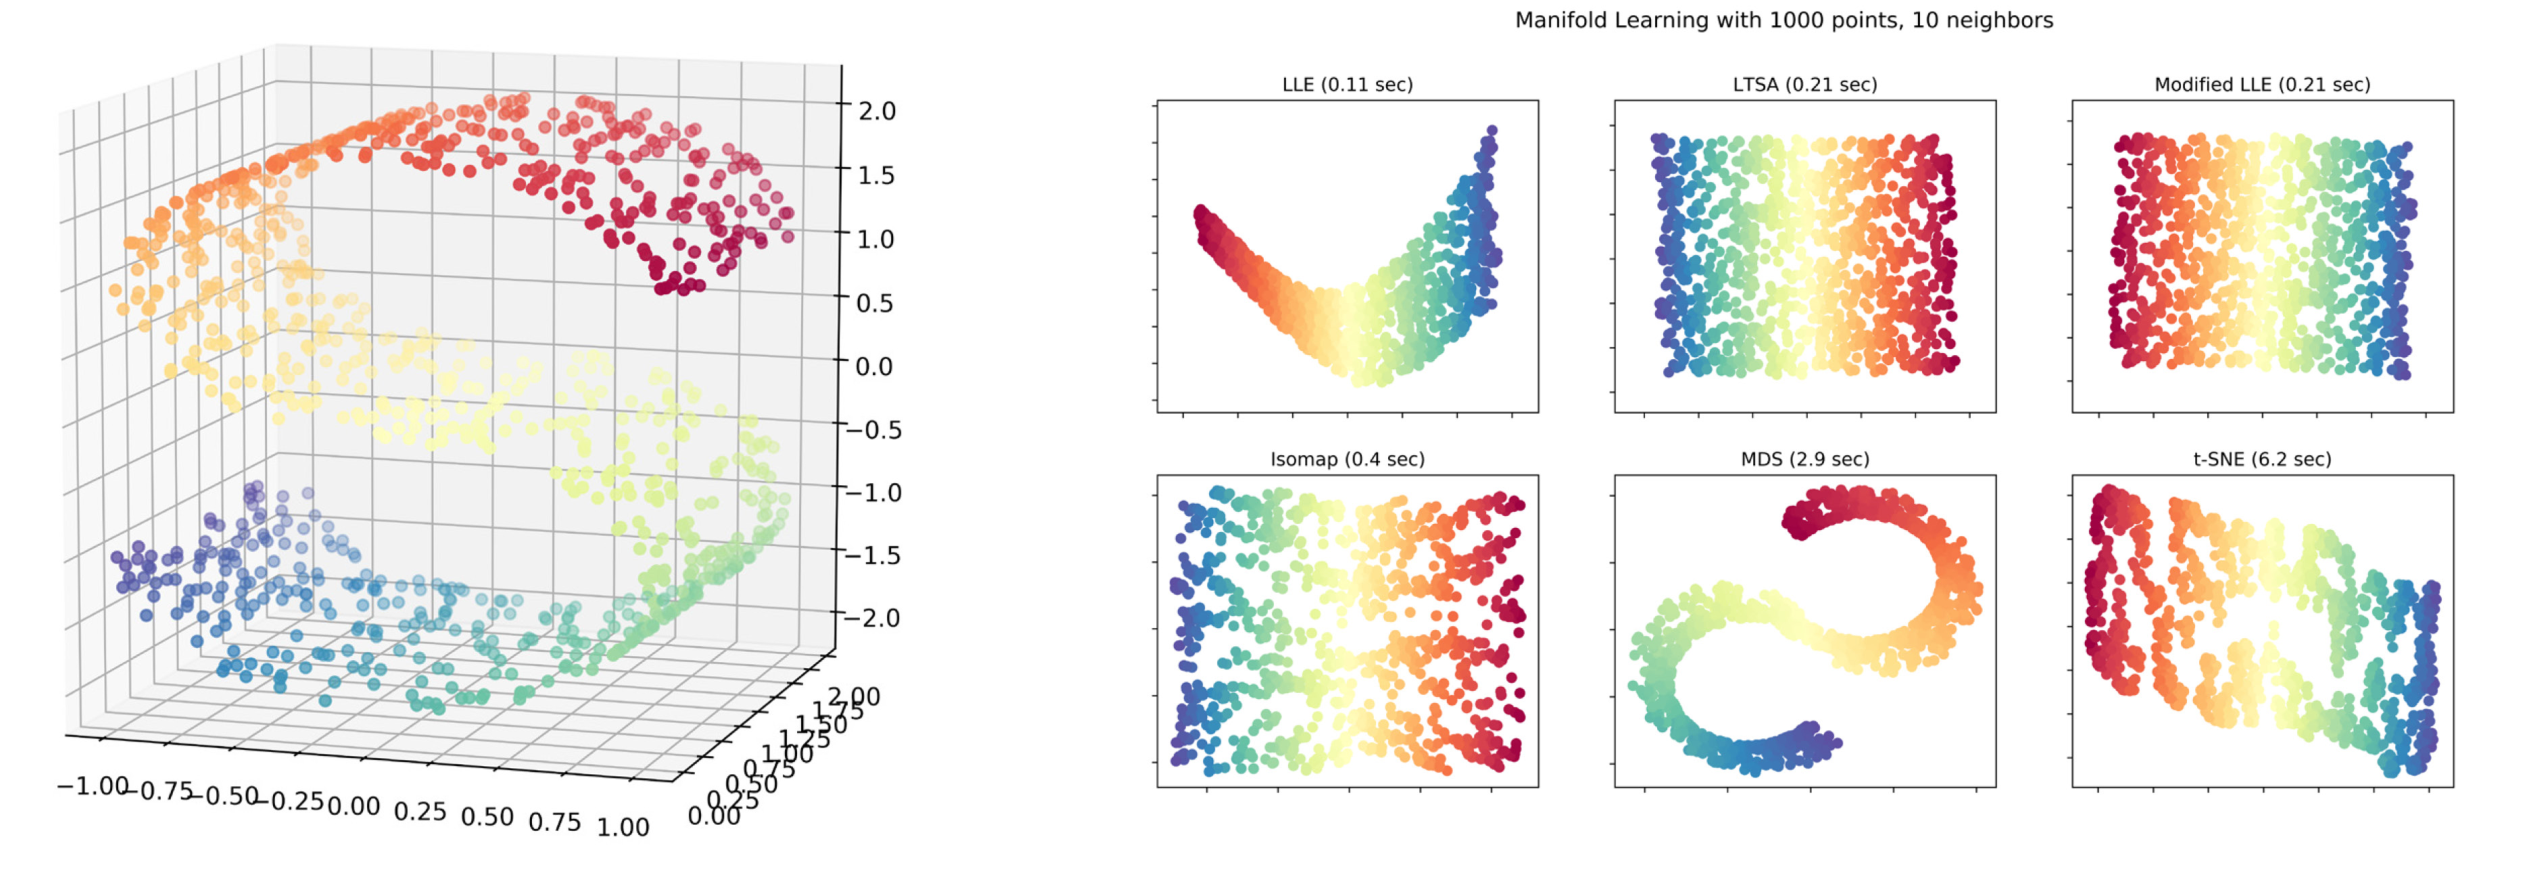
\includegraphics[width=0.8\linewidth]{img/manifold_learning}
\end{center}

\subsection{Similarity-based Methods}
Given data $\vec{\textbf{x}}$ in high dimensional space with distance. Have distances or dissimilarities $d_{ij}$ between many objects in high dimensional space and draw them in low dimensional space ($\R^2,\R^3$).
\begin{center}
	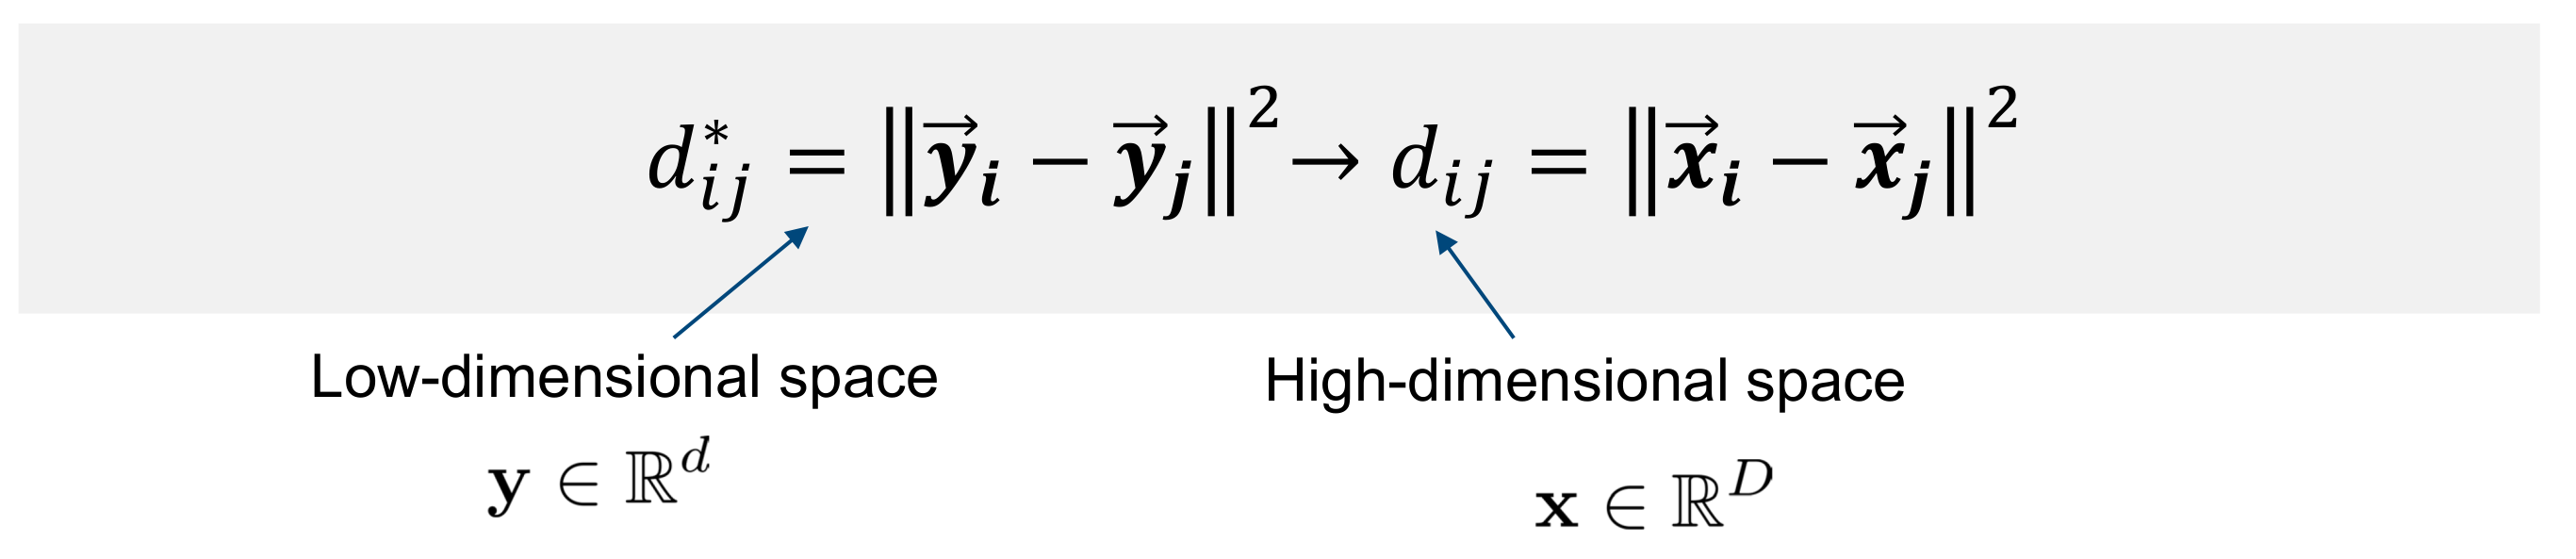
\includegraphics[width=0.8\linewidth]{img/similarity_methods}
\end{center}
The distances in low-dimensional $d_{ij}^*$ should match the original ones $d_{ij}$ in high dimensions as good as possible.

Methods:
\begin{enumerate}
	\item Multi-dimensional Scaling (\textbf{MDS})
	\item Local Linear Embedding (\textbf{LLE})
	\item Isometric Mapping (\textbf{Isomap})
	\item t-Distributed Stochastic Neighbour Embedding (\textbf{t-SNE})
\end{enumerate}
Similarity is based on a metric, a generalized form of distance measure.

\subsubsection{Similarity - A Metric and Non-Metric}
A metric $d(x,y)$ is a generalised distance measure that follows the following axioms
\begin{enumerate}
	\item \textbf{Non-negativity} $ d(x,y) \geq 0 $
	\item \textbf{Coincidence} $ d(x,y) = 0 \Leftrightarrow x = y $
	\item \textbf{Symmetry} $ d(x,y) = d(y,x) $
	\item \textbf{Triangle Inequality} $ d(x,y) + d(y,z) \geq d(x,z) $
\end{enumerate}

\vspace{1em}
\noindent
Examples of metrics
\begin{enumerate}[label=\alph*]
	\item \textbf{Euclidean} and other $L_p$-metrics\\
	Induced metric by the norm of the vector $\norm{x-y}_p$
	\item \textbf{Jaccard Distance}\\
	1 - Jaccard Index
	\item \textbf{Graph Distance}\\
	Shortest path
	\item \textbf{Wasserstein} metric\\
	Between two probability distributions
\end{enumerate}

\subsubsection{Multidimensional Scaling}
MDS reduces dimensionality while trying to preserve the distances between all the instances. It seeks a low-dimensional representation of the data in which the distances respect well the distances in the original high-dimensional space. MDS attempts \textbf{to model similarity or dissimilarity} of the data as distances in a geometric spaces. In general, is a technique used for analysing similarity or dissimilarity data.

Classical MDS takes an input matrix $I$ giving dissimilarities between pairs of items and outputs a coordinate matrix whose configuration minimizes a \textbf{loss function called strain}. Given a matrix $D = [d_{ij}]$ where $d_{ij}$ is the distance between $i$ and $j$, and wanting to find $x_i$, the \textbf{strain} is given by
\begin{align*}
	S_D(x_1,\dots,x_N) &= \left(\frac{\sum_{ij}(d_{ij} - \langle x_i|x_j\rangle)^2}{\sum_{ij}d_{ij}^2}\right)^{\frac{1}{2}}\\
	S_D(x_1,\dots,x_N) &\sim \sum_{i<j}\norm{d_ij - d_{ij}^*}
\end{align*}
MDS attempts to find an embedding from the high dimensional objects in $I$ into $x_i\in\R^N$ such that distances $d_{ij}$ are preserved.

\vspace{1em}
\noindent
\textbf{Steps of A Classical MDS Algorithm}
Classical MDS uses the fact that the coordinate matrix can be derived by an eigenvalue decomposition from $B = XX^T$. And the matrix $B$ can be computed from the proximity matrix $D$ by using \textbf{double centring}

\begin{enumerate}
	\item Set up squared proximity matrix (covariance): $C = D^{(2)} = [d_{ij}^2]$
	\item Apply double centring $B = -\frac{1}{2} HCH^T$ using the \textbf{centring matrix} $H = \mathbb{I}_n - \frac{1}{n} \mathbb{O}^T $ where $n$ is the number of objects and $\mathbb{O}$ the matrix of all ones
	\item Determine the \textbf{$m$ largest eigenvalues} and corresponding \textbf{eigenvectors} $\{u_1,\dots,u_m\}$ of $B$ ($m$ equals the output dimension)
	\item Now calculate $X = U_m (\Delta_m)^{\frac{1}{2}}$, where $U_m$ is the matrix of eigenvectors $[u_1,\dots,u_m]$ and $\Delta_m$ is the diagonal matrix of $m$ eigenvalues of $B$ 
\end{enumerate}
Classical MDS assumes \textbf{Euclidean distances}. So this is not applicable for direct dissimilarity ratings.

Example of a centring matrix in Python
\begin{minted}[fontsize=\small]{python}
H = np.eye(4) - 1/4 * np.ones((4,4))
#   array([
#   [ 0.75, -0.25, -0.25, -0.25],
#   [-0.25,  0.75, -0.25, -0.25],
#   [-0.25, -0.25,  0.75, -0.25],
#   [-0.25, -0.25, -0.25,  0.75]])
C = np.array([[1,2,3,4],[2,1,5,6],[3,5,1,7],[4,6,7,1]])
#   array([
#   [1, 2, 3, 4],
#   [2, 1, 5, 6],
#   [3, 5, 1, 7],
#   [4, 6, 7, 1]])
H*C*H.T
#   array([
#   [-0.375, -0.375,  0.125,  0.625],
#   [-0.375, -2.375,  1.125,  1.625],
#   [ 0.125,  1.125, -3.375,  2.125],
#   [ 0.625,  1.625,  2.125, -4.375]])
\end{minted}

\paragraph{Summary of MDS}
\begin{itemize}
	\item MDS is fast, because it is based on linear algebra
	\item Only distances are needed as input (as all MDS methods)
	\item The formulation as a cost function is valid for Euclidean distances only (internally Eigenvalues are used). If other distances (besides Euclidean) are used, nothing is guaranteed.
	\item MDS tries to preserve the distance between all data points, even if they are far separated.
	\item For Euclidean distances, classical MDS is equivalent to PCA	
\end{itemize}

\subsubsection{Local Linear Embedding}
LLE reduces dimensionality while trying to preserve the distances between close instances only. It describes the local properties of the manifold around a data point $x_i$ by writing the data point as a linear combination (the so-called reconstruction weights $w_{ij}$) of its $k$ \emph{nearest neighbours}
\begin{equation}
	x_i \approx \sum_j w_{ij} x_j
	\label{eq:LLEnearestneighbours}
\end{equation}
In the low dimension LLE attempts to \textbf{retain the reconstruction weights $W$ as well as possible}. Hence, this method fits a hyperplane through the data point $x_i$ and its nearest neighbours, thereby \textbf{assuming that he manifold is locally linear}.

The local linearity assumption implies that the reconstruction weights $ w_{ij} $ of the data points $x_i$ are \textbf{invariant to translation, rotation, and rescaling}. Because of the invariance to these transformations, any linear mapping of the hyperplane to a space of lower dimensionality preserves the reconstruction weights in the space of lower dimensionality.

As a consequence, finding the $d$-dimensional data representation $Y$ amounts to minimising the cost function $\phi$:
\begin{equation*}
	\phi(Y) = \sum_{i}\left(y_i - \sum_{j=1}^{k}w_{ij}y_j\right)^2
\end{equation*}
For each training instance $x_i$, the algorithm identifies its $k$ closest neighbours, then tries to reconstruct $x_i$ as a linear function of these neighbours (see equation \ref{eq:LLEnearestneighbours}). More specifically, it finds the weights $w_{ij}$ such that the squared distance between $x_i$ and $\sum_j w_{ij} x_j$ is as small as possible, assuming $w_{ij} = 0$ if $x_j$ is note one of the $k$ closest neighbours of $x_i$. Thus the first step of LLE is the \textbf{constrained optimisation problem} where $W$ is the weight matrix containing all the weights $w_{ij}$.

The second constraint simply normalises the weights for each training instance $x_i$
\begin{align*}
	\widehat{W} &= \argmin{W}\left\{ \sum_{i=1}^{m}\norm{x_i - \sum_j w_{ij}x_j}^2 \right\}\\
	\text{subject to} \quad &\begin{cases}
	w_{ij} = 0 & \text{if $x_j$ is not one of the $k$-nearest neighbours of $x_i$}\\
	\sum_{j=1}^{m} w_{ij} = 1 & (i=1\dots m)
	\end{cases}
\end{align*}

\subsubsection{Isomap}
Isomap creates a graph by connecting each instance to its nearest neighbours, then reduces dimensionality while trying to preserve the geodesic distances between the instances. It is a \textbf{non-linear method} for dimensionality reduction and finds the that preserves the global, non-linear geometry of the data by \textbf{preserving the geodesic manifold inter-point distances}. A geodesic is the shortest curve along the manifold connecting two points.

This method first approximates the geodesic inter-point distances and then runs MDS to find the projection that preserves these distances. Thus, it uses the same basic idea as PCA, but preserves linearity only locally via small neighbourhoods.

\begin{enumerate}
	\item For each object, find a small set of neighbouring objects and their distances
	\item Compute \emph{all-pairs shortest paths} on the above neighbourhood graph
	\item Run \emph{multidimensional scaling} using the matrix of shortest-path distances
\end{enumerate}

\begin{figure}[H]
	\centering
	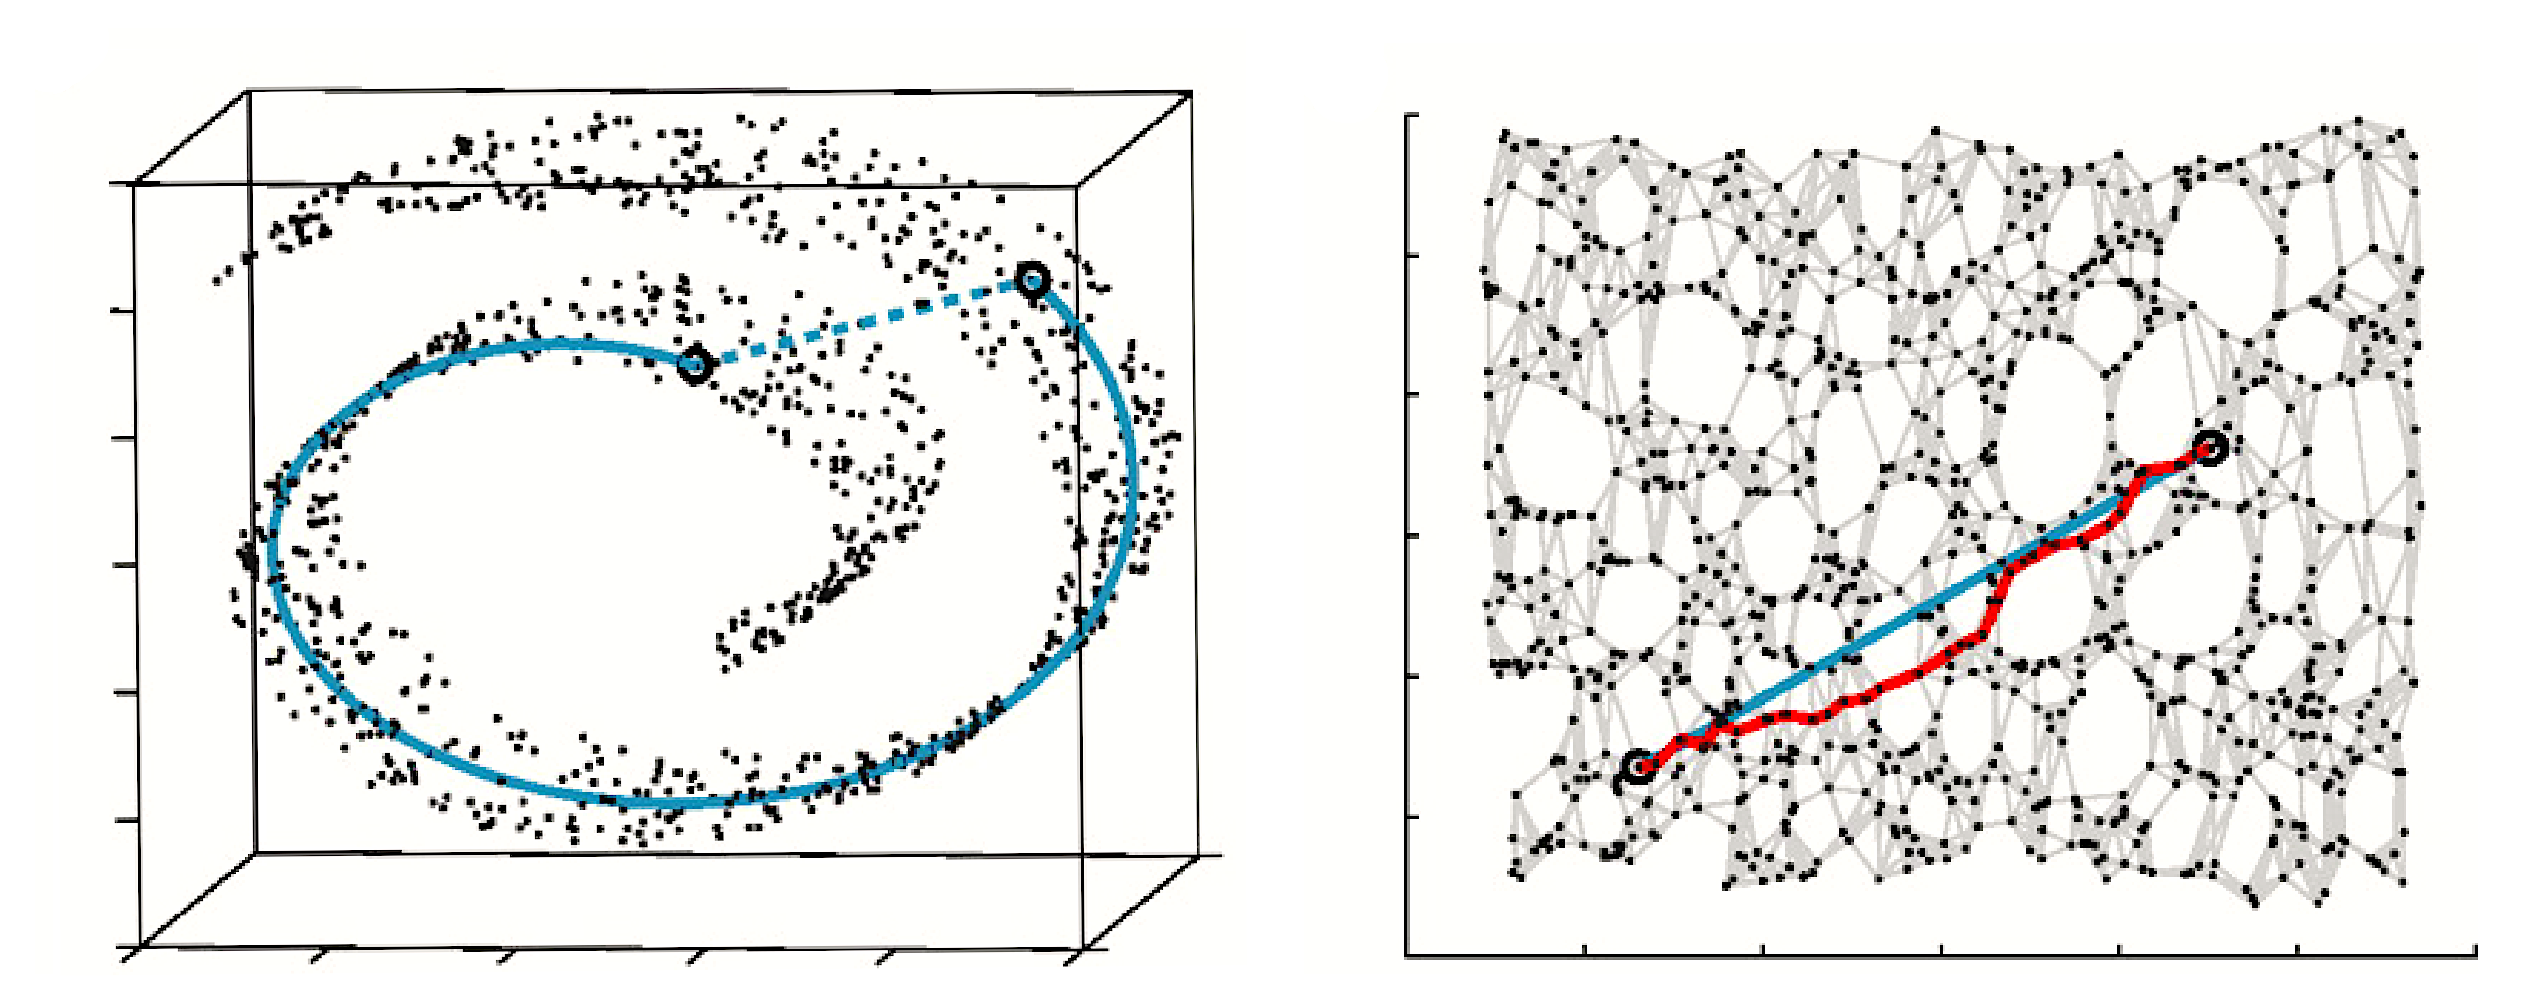
\includegraphics[width=0.8\linewidth]{img/isomap}
	\caption{Graph geodesic: In the field of graph theory, the distance between two vertices in a graph is the number of edges in a shortest path connecting them. This is also known as the geodesic distance.}
	\label{fig:isomap}
\end{figure}

\subsubsection{t-Distributed Stochastic Neighbour Embedding}
t-SNE reduces dimensionality while trying to keep similar instances close and dissimilar instances apart. It is mostly used for visualization, in particular to visualize clusters of instances in high-dimensional space. It is a manifold learning algorithm that in essence constructs a probability distribution $p$ over the dataset $X$, and then another probability distribution $q$ in a lower dimensional data space $Y$, making both distributions as similar to each other as possible.

t-SNE uses a tuneable parameter \textbf{perplexity}, which defines how to balance attention between local and global aspects of the data. The parameter can be understood as a guess about the number of \emph{close} neighbours each point has. This method is incredibly flexible and can often find structures in the data, where other dimensionality reduction algorithms fail to do. Unfortunately, this flexibility is gained at the cost of interpretability.

\begin{enumerate}
	\item In the high dimensional space $X$, create a probability distribution $p_{i|j}$ that dictates the relationships between various neighbouring points $x_i$ and $x_j$
	\item Try to recreate a probability distribution $q_{i|j}$ in a low dimensional space $Y$ that follows that probability distribution $p_{i|j}$ as best as possible. Use Kullback–Leibler divergence as loss function
\end{enumerate}

\paragraph{Stochastic Neighbour Embedding} constructs a probability distribution $q$ in the lower dimensional space using the following formula for pairwise points $y$
\begin{align*}
	p_{i|j} &= \frac{e^{-\frac{\norm{x_i - x_j}^2}{2\sigma_i^2}}}{\sum_{k\neq i}e^{-\frac{\norm{x_i - x_k}^2}{2\sigma_i^2}}}\\
	q_{i|j} &= \frac{e^{-\norm{y_i - y_j}^2}}{\sum_{k\neq i}e^{\norm{y_i - y_k}^2}}
\end{align*}
The goal is to make sure the two probability distributions are as similar as possible. This is achieved by considering the \textbf{Kullback-Leibler divergence}, which is a measure of how different two probability distributions are from one another
\begin{equation}
	\text{KL}(P|Q) = \sum_{i\neq j} p_{i|j} ln\left(\frac{p_{i|j}}{q_{i|j}}\right)
\end{equation}
In essence, the KL divergence is the expected value of the log difference of the probabilities of the data points.

\subsubsection{Linear Discriminant Analysis}
LDA is actually a classification algorithm. During training it learns the most discriminative axes between the classes. These axes can be used to define a hyperplane onto which to project the data. The projection will keep classes as far apart as possible, so LDA is a good technique to reduce dimensionality before running another classification algorithm such as an SVM classifier.

\section{Clustering}
Clustering is finding groups in data. Given $n$ data points, separate them into $K$ clusters ($n$: number of data points, $K$: number of clusters, $\Delta$: a partition $\Delta = \{C_1, C_2,\dots, C_K\}$, $\mathcal{L}(\Delta)$: loss of $\Delta$ to be minimised). There is a differentiation between hard clustering, where each data point is assigned to a unique cluster, and soft clustering, where each data point $i$ is assigned a probability that it is in cluster $k:=\{\gamma_{ki}\}_{k=1:K}$. Clustering is related to vector quantisation.

\subsection{Taxonomy of Clustering}
\begin{itemize}
	\item \textbf{Parametric clustering}: $K$ known
	\item \textbf{Non-parametric clustering}: $K$ determined by algorithm
\end{itemize}
\textbf{Hierarchical Clustering} (HCA) seeks to build a hierarchy of clusters. Strategies for hierarchical clustering generally fall into two types
\begin{itemize}
	\item \textbf{Agglomerative}, a bottom-up approach where each observation starts in its own cluster, and pairs of clusters are merged the longer the algorithm is run
	\item \textbf{Divisive}, a top-down approach where all observations start in one cluster and splits are performed recursively as the algorithm moves down the hierarchy
\end{itemize}
In hierarchical clustering, clusters have a tree like structure or a \emph{parent child relationship}. Here, the two most similar clusters are combined together and continue to combine until all objects are in the same cluster.

\subsubsection{Other Distinctions}
\begin{itemize}
	\item \textbf{Exclusive versus non-exclusive}, where in non-exclusive clusterings points may belong to multiple clusters
	\item \textbf{Fuzzy versus non-fuzzy}, where in fuzzy clustering a point belongs to every cluster with some weight between 0 and 1, who must sum up to 1. Probabilistic clustering has similar characteristics
	\item \textbf{Partial versus complete}, where in the partial case not the whole dataset is used
	\item \textbf{Heterogeneous versus non-heterogeneous}, where clusters can have widely different sizes, shapes or densities
\end{itemize}

\subsection{Hierarchical Clustering}
In order to decide which clusters should be combined or where a cluster should be split, a measure of dissimilarity between sets of observations is required. In most methods of hierarchical clustering, this is achieved by use of an appropriate \textbf{metric} (a measure of distance between pairs of observations), and a \textbf{linkage criterion} which specifies the dissimilarity of sets as a function of the pairwise distances of observations in the sets.

In agglomerative clustering there are $N$ data points at the start that initially form $N$ clusters. The two clusters with the smallest linkage are fused together to form $N-1$ clusters. This is repeated until there is only one single cluster.
\begin{equation*}
	(i,j)_{\text{fused}} = \underset{i\neq j}{\text{argmin}} \left\{ D_{\text{link}})(C_i,C_j) \right\}
\end{equation*}

\vspace{1em}
\noindent
A \textbf{metric} d(x,y) is a generalised distance measure that follows these axioms
\begin{tabularx}{\linewidth}{l X}
	1. Non-negativity & $d(x,y)\geq 0$\\
	2. Coincidence & $d(x,y) = 0 \Leftrightarrow x=y$\\
	3. Symmetry & $d(x,y) = d(y,x)$\\
	4. Triangle inequality & $d(x,y) + d(y,z) \geq d(x,z)$
\end{tabularx}
\begin{itemize}
	\item $L_p$ metric: \quad $d_p(x,y) = \norm{x-y}_p = \sqrt[p]{\sum_i \abs{x_i - y_i}^p}$
	\item $L_\infty$ metric: \quad $\norm{x}_\infty = \max_i\left\{\abs{x_i}\right\}$
	\item $L_1$ metric: \quad $d_1(x,y) = \norm{x-y}_1 = \sum_i\abs{x_i - y_i}$
\end{itemize}
\clearpage
The linkage criterion determines together with a metric $d(x,y)$ when two clusters $A$ and $B$ should be merged together in hierarchical clustering (fusion criterium).
\begin{tabularx}{\linewidth}{m{0.35\linewidth} m{0.35\linewidth} m{0.2\linewidth}}
	\textbf{Names} & \textbf{Formula} & \textbf{Plot}\\
	\hline
	&&\\[-0.5em]
	\textbf{Maximum} or complete-linkage clustering & $ \max\left\{ d(a,b):a\in A, b\in B \right\} $ & 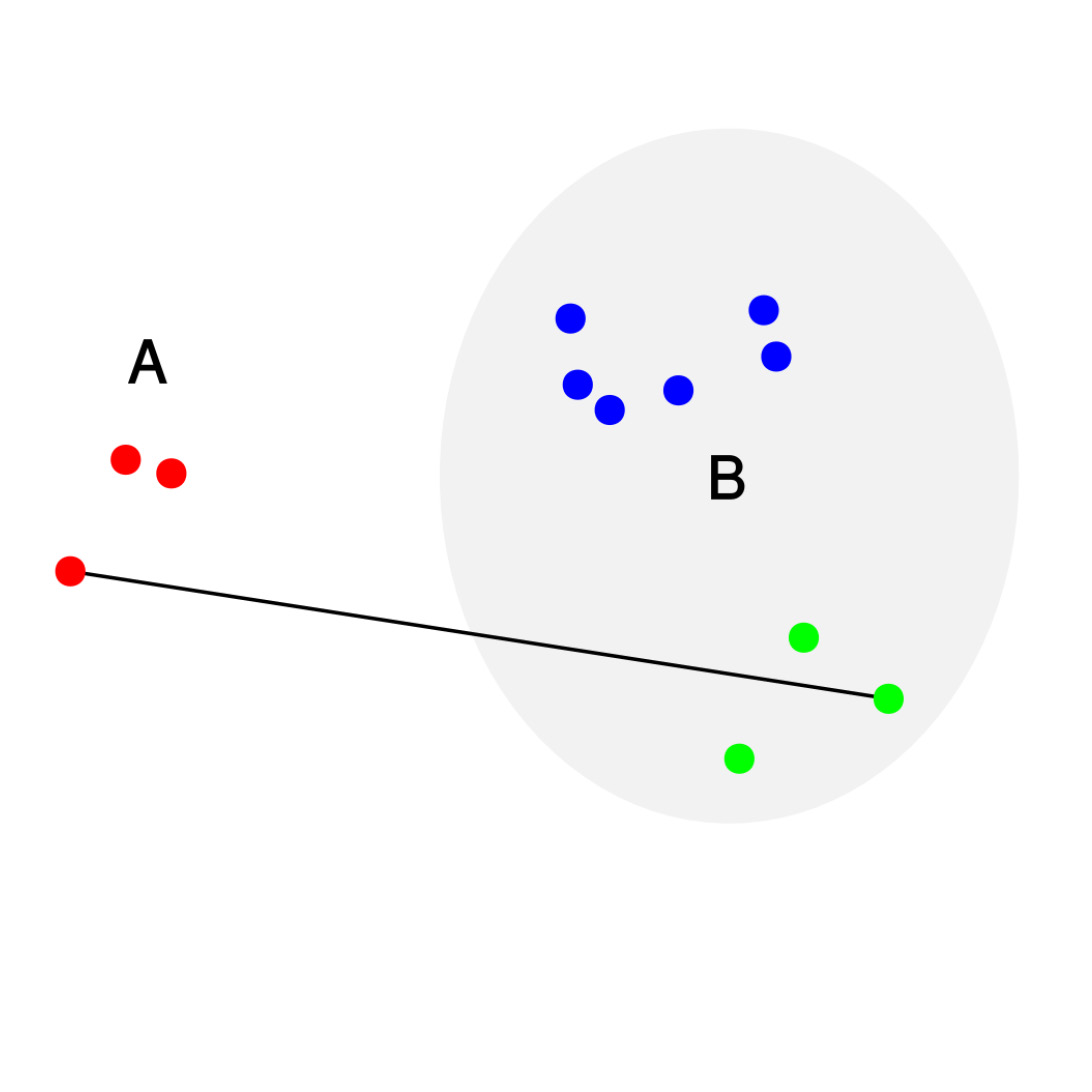
\includegraphics[width=\linewidth]{complete_linkage}\\
	\textbf{Minimum} or single-linkage clustering & $ \min\left\{ d(a,b):a\in A, b\in B \right\} $ & 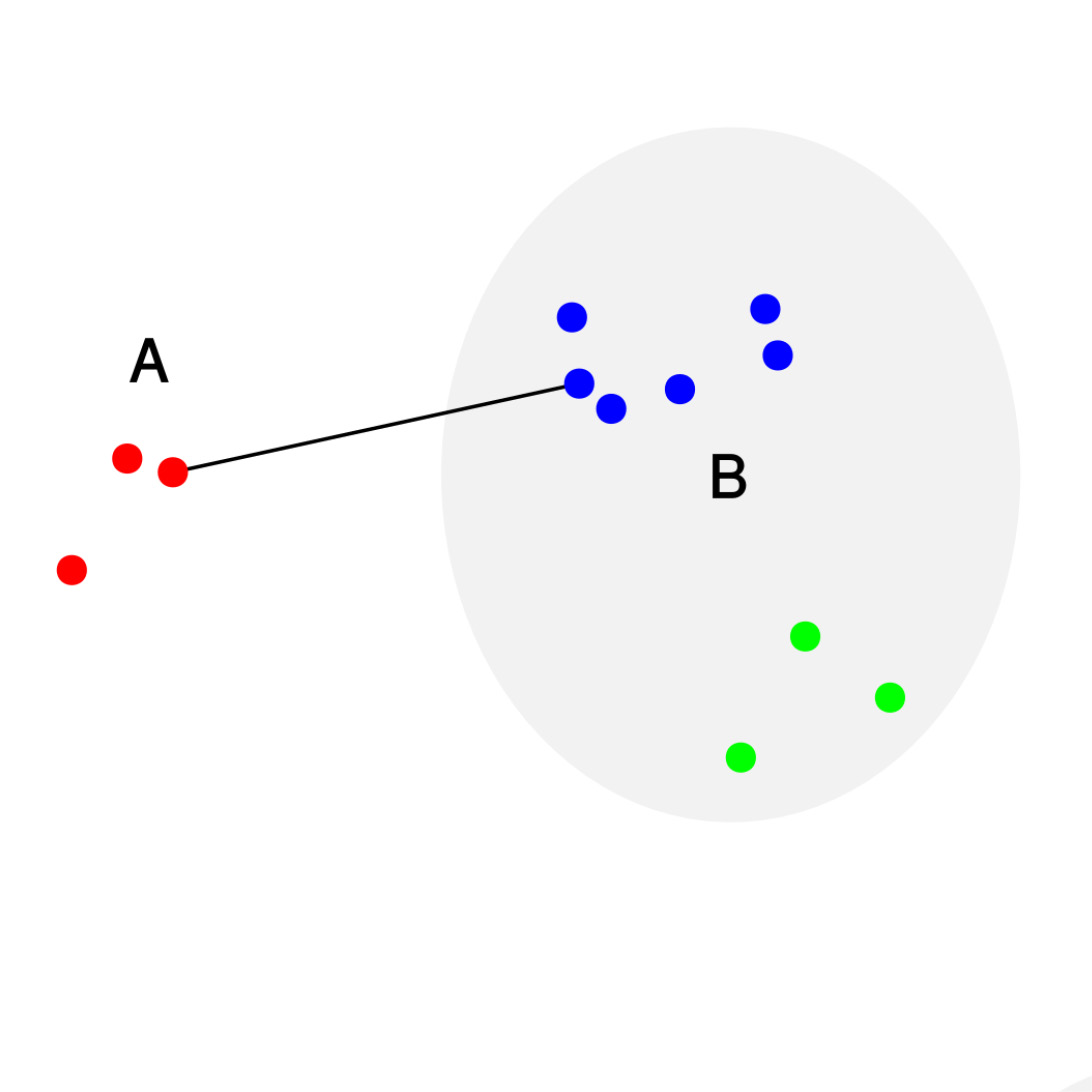
\includegraphics[width=\linewidth]{single_linkage}\\
	\textbf{Mean}, average-linkage clustering or UPGMA & $ \frac{1}{\abs{A}\cdot\abs{B}}\sum_{a\in A}\sum_{b\in B} d(a,b) $ & 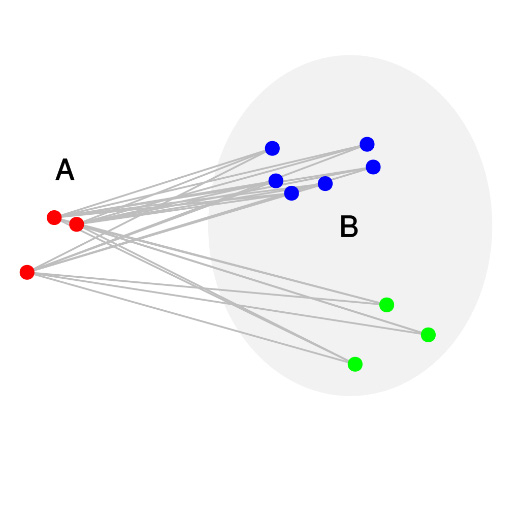
\includegraphics[width=\linewidth]{img/average_linkage}\\
	\textbf{Ward} linkage & $D_{\text{Ward}}(A,B) := \frac{d(\bar{a},\bar{b})^2}{\dfrac{1}{\abs{A}} + \dfrac{1}{\abs{B}}}$; increase of variance when fusing $A$ and $B$ & \\
	\textbf{Maximum} or complete-linkage clustering & $ \norm{c_s - c_t} $, where $c_s$ and $c_t$ are the centroids of clusters $s$ and $t$ & 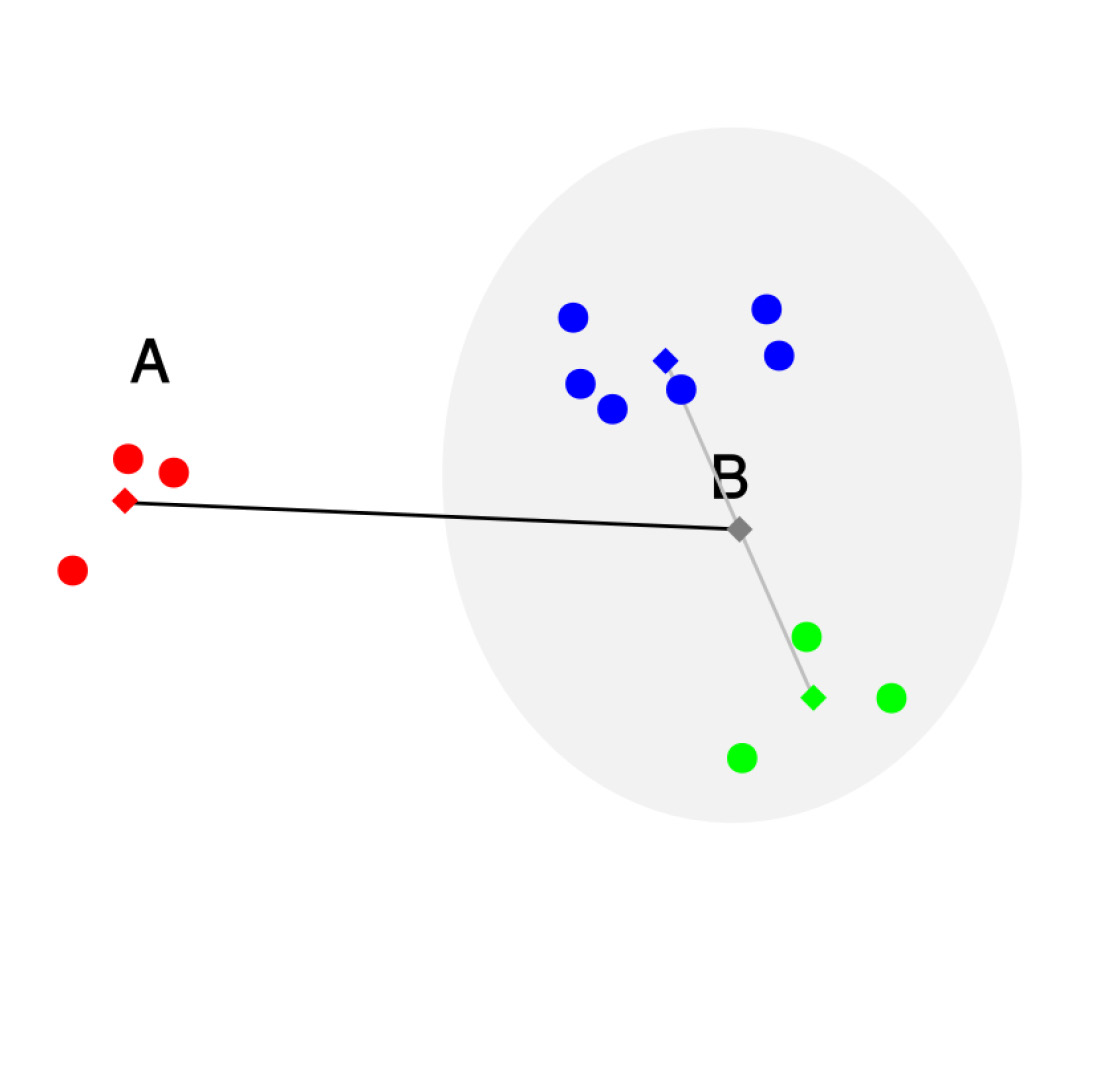
\includegraphics[width=\linewidth]{img/centroid_linkage}
\end{tabularx}

\subsubsection{Basic Form of an Agglomerative Linkage Algorithm}
\textbf{Input}:
\begin{itemize}[nosep]
	\item Distance matrix $D$ between data points
	\item function \texttt{dist} to compute a distance between clusters (which usually takes $D$ as an input)
\end{itemize}
\textbf{Initialisation}: Clustering $\mathcal{C}^{(0)} = \left\{ C_1^{(0)}, C_2^{(0)},\dots, C_n^{(0)} \right\} = \{i\}$
\begin{itemize}
	\item \textbf{While} the current number of clusters is $>1$:
	\begin{itemize}[nosep]
		\item find the two clusters which have the \textbf{smallest distance (linkage)} to each other
		\item \textbf{merge} them to one cluster
	\end{itemize}
	\item \textbf{Output}: Resulting \textbf{dendogram}, which is a tree that represents the hierarchical division of the data set $O$ into ever smaller subsets.
\end{itemize}

\begin{minted}[linenos]{python}
# Import dendrogram and ward clustering from SciPy
from scipy.cluster.hierarchy import dendrogram, ward
X, y = make_blobs(random_state=0, n_samples=12)
#Perform ward clustering on the data in array X. The function ward in SciPy
returns an array with the #distances bridged in agglomerative clustering
linkage_array = ward(X)
# draw a dendrogram
dendrogram(linkage_array)
\end{minted}
\begin{center}
	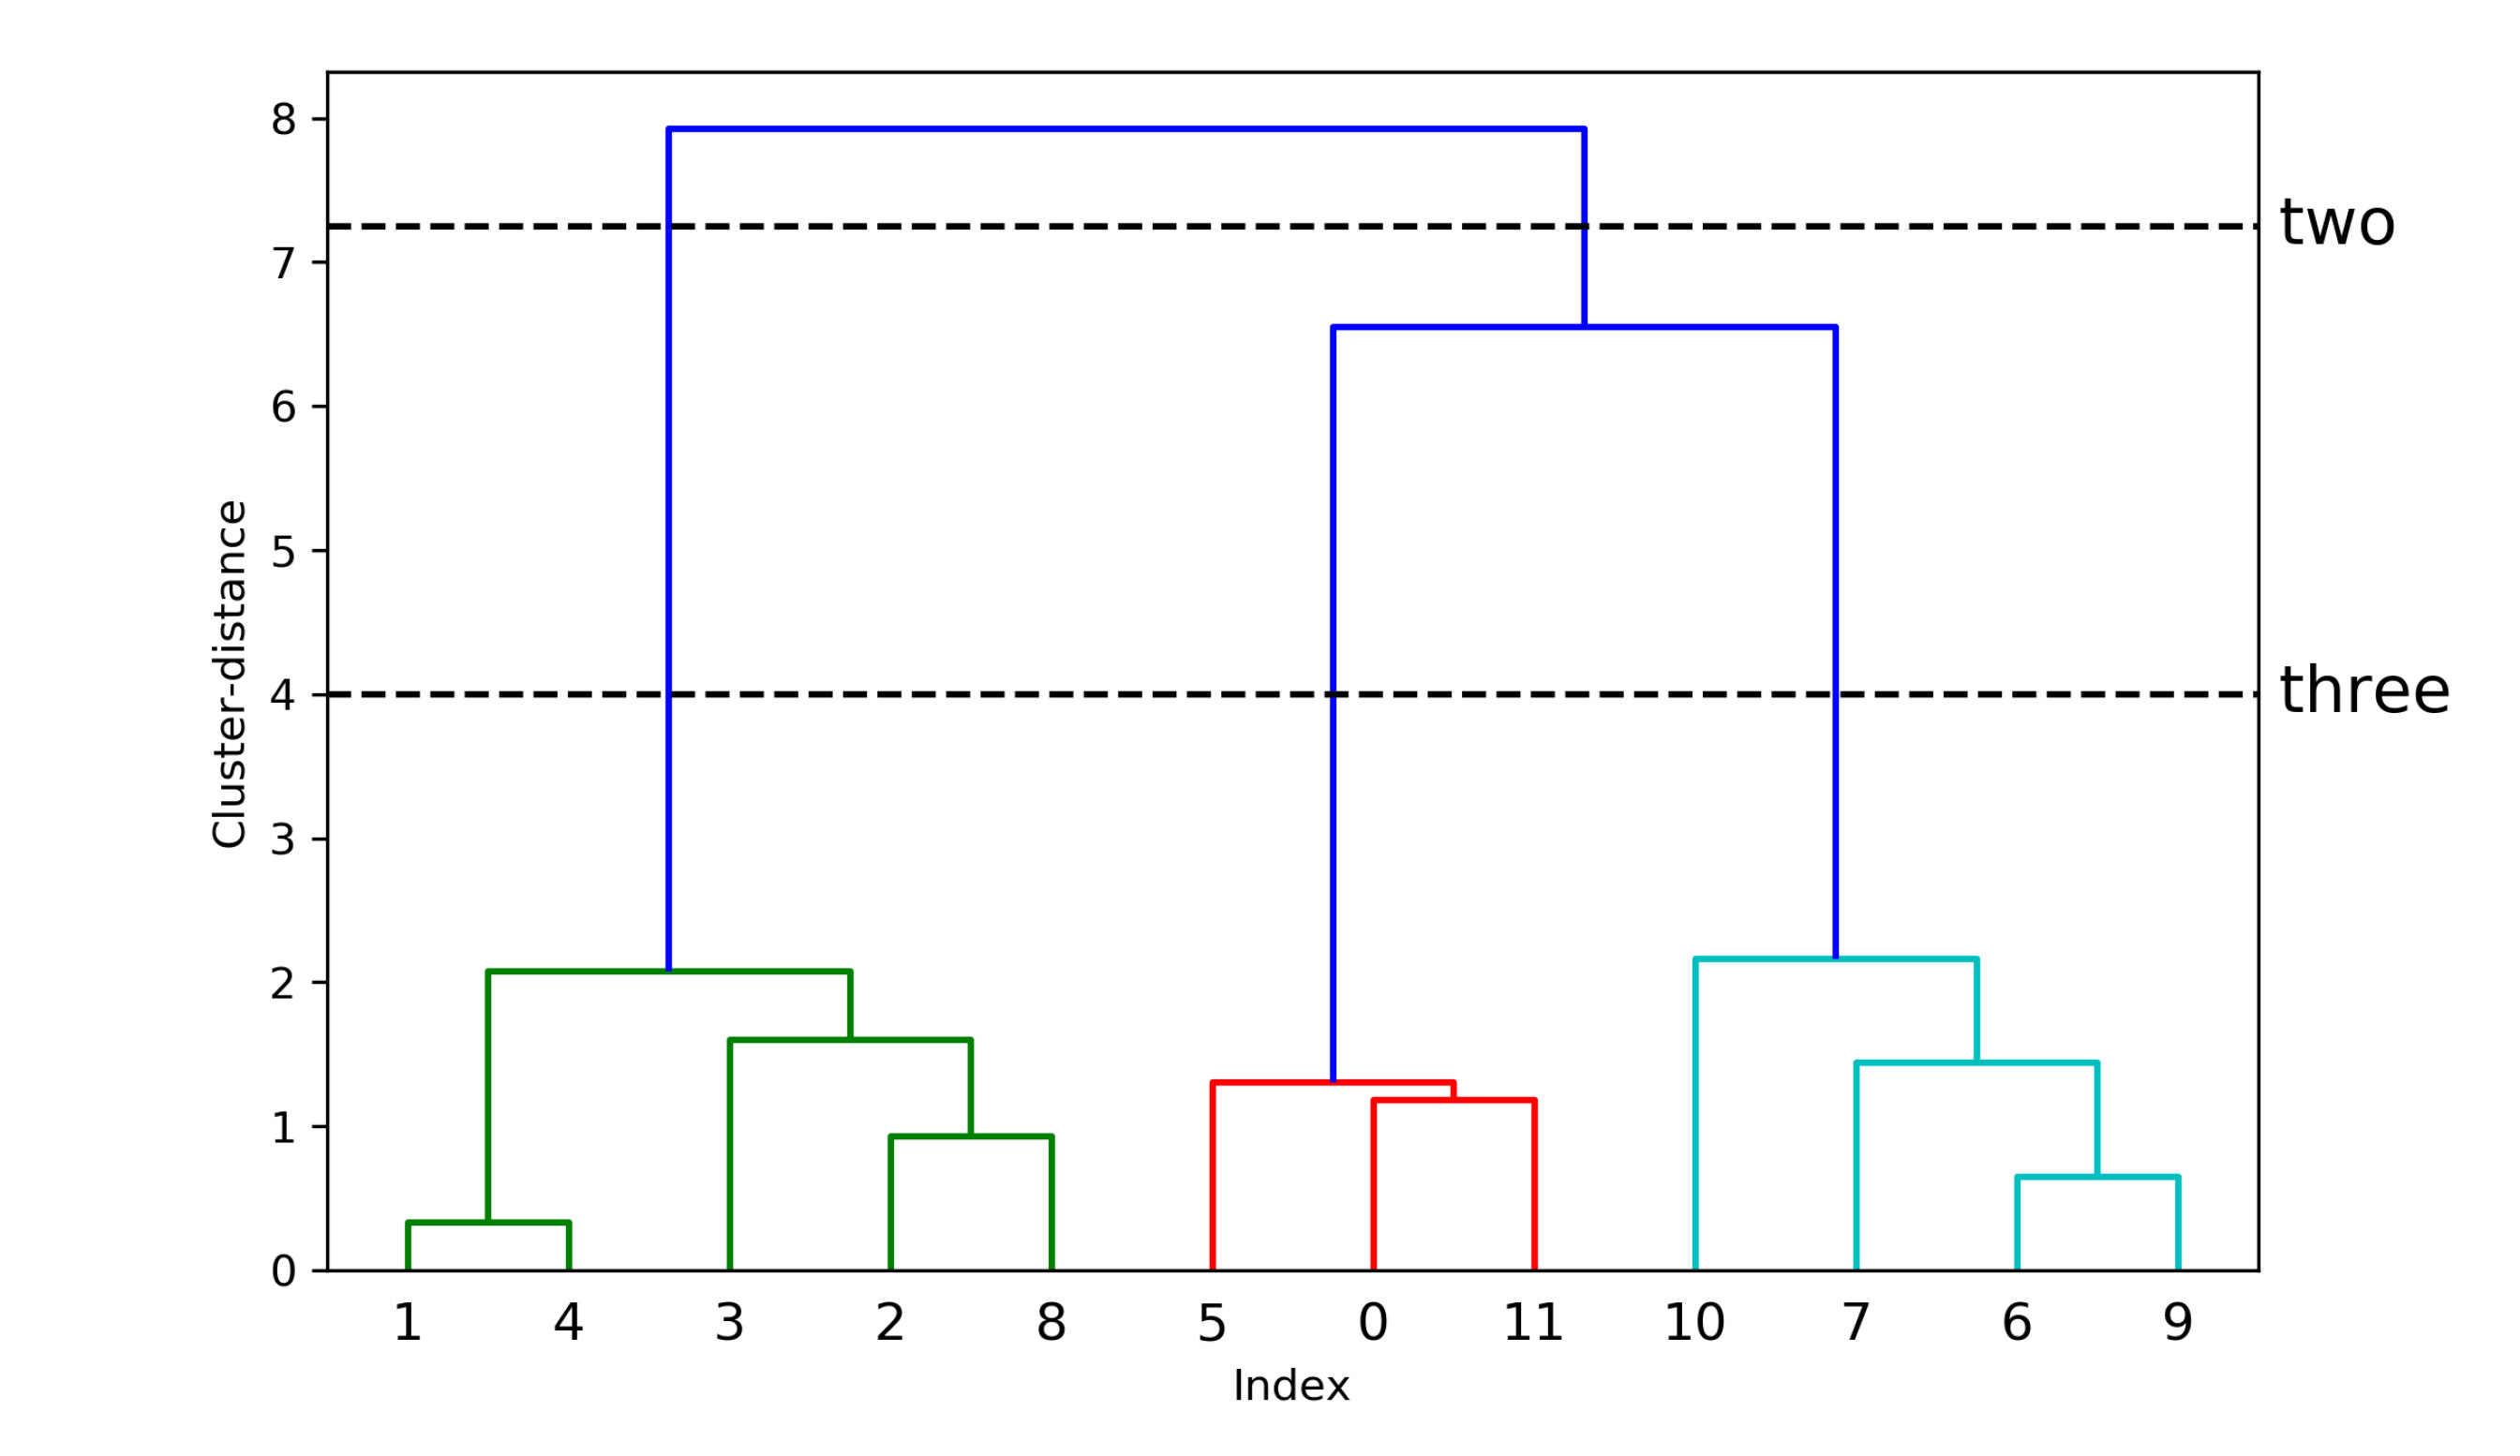
\includegraphics[width=0.7\linewidth]{img/dendrogram}
\end{center}

\subsubsection{Divisive Clustering - Single Linkage Algorithm Based on Minimum Spanning Tree}
\textbf{Input}: Data $D = \{ x_i \}_{i=1:N}$ and number of clusters $K$
\begin{enumerate}
	\item Construct the Minimum Spanning Tree (MST) of $D$
	\item Delete the largest $(K-1)$ edges
\end{enumerate}
\textbf{Cost}:
\begin{align}
	\mathcal{L}(\Delta) &= \underset{k,k'}{\min}d(C_k, C_{k'})\\
	d(A,B) = \underset{x\in A, y\in B}{\min}\norm{x-y}
\end{align}
This method is sensitive to outliers, but the cost can be evaluated in polynomial time $O(n^2)$.

\subsection{K-Means}
\begin{figure}[H]
	\begin{subfigure}{0.45\linewidth}
		\centering
		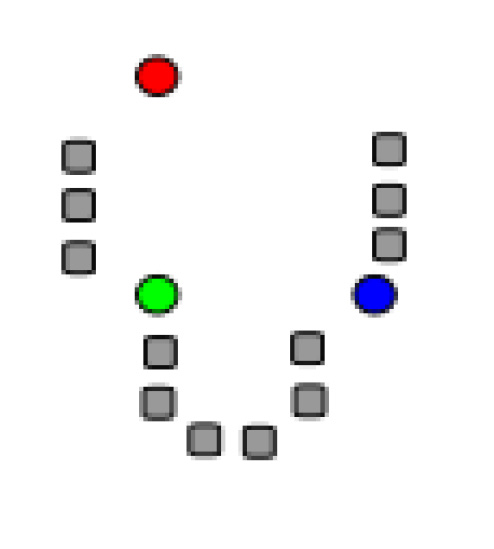
\includegraphics[width=3cm]{kmeans01}
		\caption{$k$ initial "means" are randomly generated within the data domain}
	\end{subfigure}
	\hspace{\fill}
	\begin{subfigure}{0.45\linewidth}
		\centering
		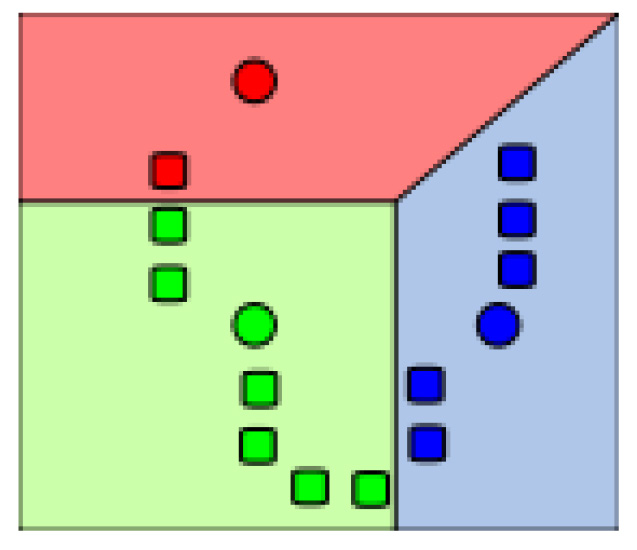
\includegraphics[width=3cm]{kmeans02}
		\caption{$k$ clusters are created by associating every observation with the nearest mean. The partitions here represent the Voronoi diagram generated by the means.}
	\end{subfigure}
	\begin{subfigure}{0.45\linewidth}
		\centering
		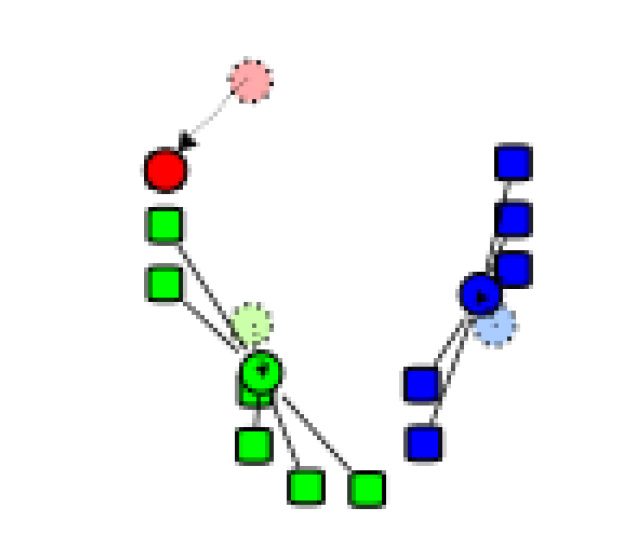
\includegraphics[width=3cm]{kmeans03}
		\caption{The centroid of each of the $k$ clusters becomes the new mean}
	\end{subfigure}
	\hspace{\fill}
	\begin{subfigure}{0.45\linewidth}
		\centering
		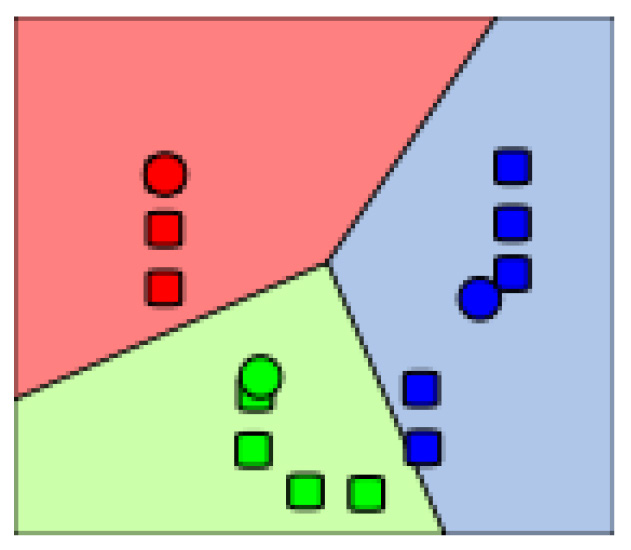
\includegraphics[width=3cm]{kmeans04}
		\caption{The preceding steps are repeated until convergence has been reached}
	\end{subfigure}
\end{figure}

\subsubsection{Algorithm}
\begin{itemize}
	\item \textbf{Input}: Data $D = \{ x_i \}_{i=1:N}$ and number of clusters $K$
	\item \textbf{Initialise}: centers $\mu_1,\mu_2,\dots,\mu_k \in \R^d$ at random
	\item Iterate until convergence
	\begin{enumerate}
		\item \texttt{for} $i=1:n$\\
		$k(i) = \text{argmin}_k\norm{x_i - \mu_k}$ (assign points to cluster to get a new clustering)
		\item \texttt{for} $i=1:n$\\
		\begin{equation*}
			\mu_k = \frac{1}{\abs{C_k}}\sum_{i\in C_k} x_i
		\end{equation*}
		(recalculate centres)
	\end{enumerate}
	\item \textbf{Convergence}: if $\Delta$ does not change after iteration $m$, it will never change after that
\end{itemize}

\subsubsection{Cost Function}
The least-squares cost function is also called \textbf{distortion} (within cluster inertia $W$)
\begin{align*}
	\mathcal{L}(\Delta) &= \sum_{i=1}^{n}\norm{x_i - \mu_{k(i)}}^2\\
	&= \sum_{k=1}^{K}\sum_{i\in C_k} \norm{x_i - \mu_{k(i)}}^2
\end{align*}
The distortion can also be expressed as \textbf{sum of (squared) intra-cluster distances}
\begin{equation*}
	\mathcal{L}(\Delta) = \frac{1}{2} \sum_{k=1}^{K}\sum_{i\in C_k} \norm{x_i - x_j}^2 + \text{constant}
\end{equation*}

\subsubsection{Initialisation}
\textbf{Random Initialisation}
\begin{itemize}[nosep]
	\item Most common: randomly choose some data points as starting centers.
	\item Draw starting points randomly from $\R^d$
	\item Initialize the centers using the solution of an even simpler clustering algorithm
	\item Ideally have prior knowledge, for example that certain points are in different clusters
\end{itemize}

\subsubsection{More Variants}
\begin{itemize}
	\item \textbf{K-Medians}: The median is computed in each single dimension in the Manhattan-distance formulation of the k-medians algorithm
	\item \textbf{Weighted K-Means}: introduce weights for the individual data points
	\item \textbf{Kernel-K-Means}: the kernelized version of K-means
	\item \textbf{Soft K-Means}: no hard assignments, but soft assignments
\end{itemize}

\subsubsection{K-Medoid and K-Maxoid Clustering}
The \textbf{medoid} $\textbf{m}$ of \X coincides with the data point $x_j \in \X$ that is closest to the mean $\mu$. The point $x_j \in X$ with the smallest average distance to all other points in \X is closest to the sample mean $\mu$. The \textbf{maxoid} is the point farthest from the mean and thus the one with the largest average distance to all points closest to the sample mean.
\begin{align*}
	\text{Medoid:}\qquad \textbf{m} &= \argmin{\textbf{x}_l} \frac{1}{n} \sum_{i=1}^{n}\norm{\textbf{x}_l - \textbf{x}_i}^2\\
	\text{Maxoid:}\qquad \textbf{m} &= \argmax{\textbf{x}_l} \frac{1}{n} \sum_{i=1}^{n}\norm{\textbf{x}_l - \textbf{x}_i}^2
\end{align*}
Contrary to the $\mu_k$ in K-Means, the $m_k$ in K-medoids or maxoids are guaranteed to coincide with data points so that \textbf{K-medoids or -maxoids clustering exclusively relies on distance between data points}. All distances evaluated during these methods can therefore be precomputed and stored in a distance matrix $\textbf{D}$ where
\begin{equation*}
	\textbf{D}_{ij} = \norm{\textbf{x}_i - \textbf{x}_j}^2
\end{equation*}

\subsubsection{Heuristics for Result Improvement}
\begin{itemize}
	\item \textbf{Restart} many times with different initializations.
	\item \textbf{Swap} individual points between clusters.
	\item \textbf{Remove a cluster centre}, and introduce a completely new centre instead.
	\item \textbf{Merge clusters} and additionally introduce a completely new cluster centre.
	\item \textbf{Split a cluster in two pieces}, preferably one which has a bad objective function. Then, reduce the number of clusters again, for example by randomly removing one.
	\item Choose $K$ by using the \textbf{elbow method} or preferably by using \textbf{Cross-Validation}
	\begin{itemize}
		\item Repeatedly split the data into training and validation datasets
		\item Cluster the training dataset
		\item Measure average distance to centres on validation data
	\end{itemize}
\end{itemize}

\begin{figure}[tbh]
	\centering
	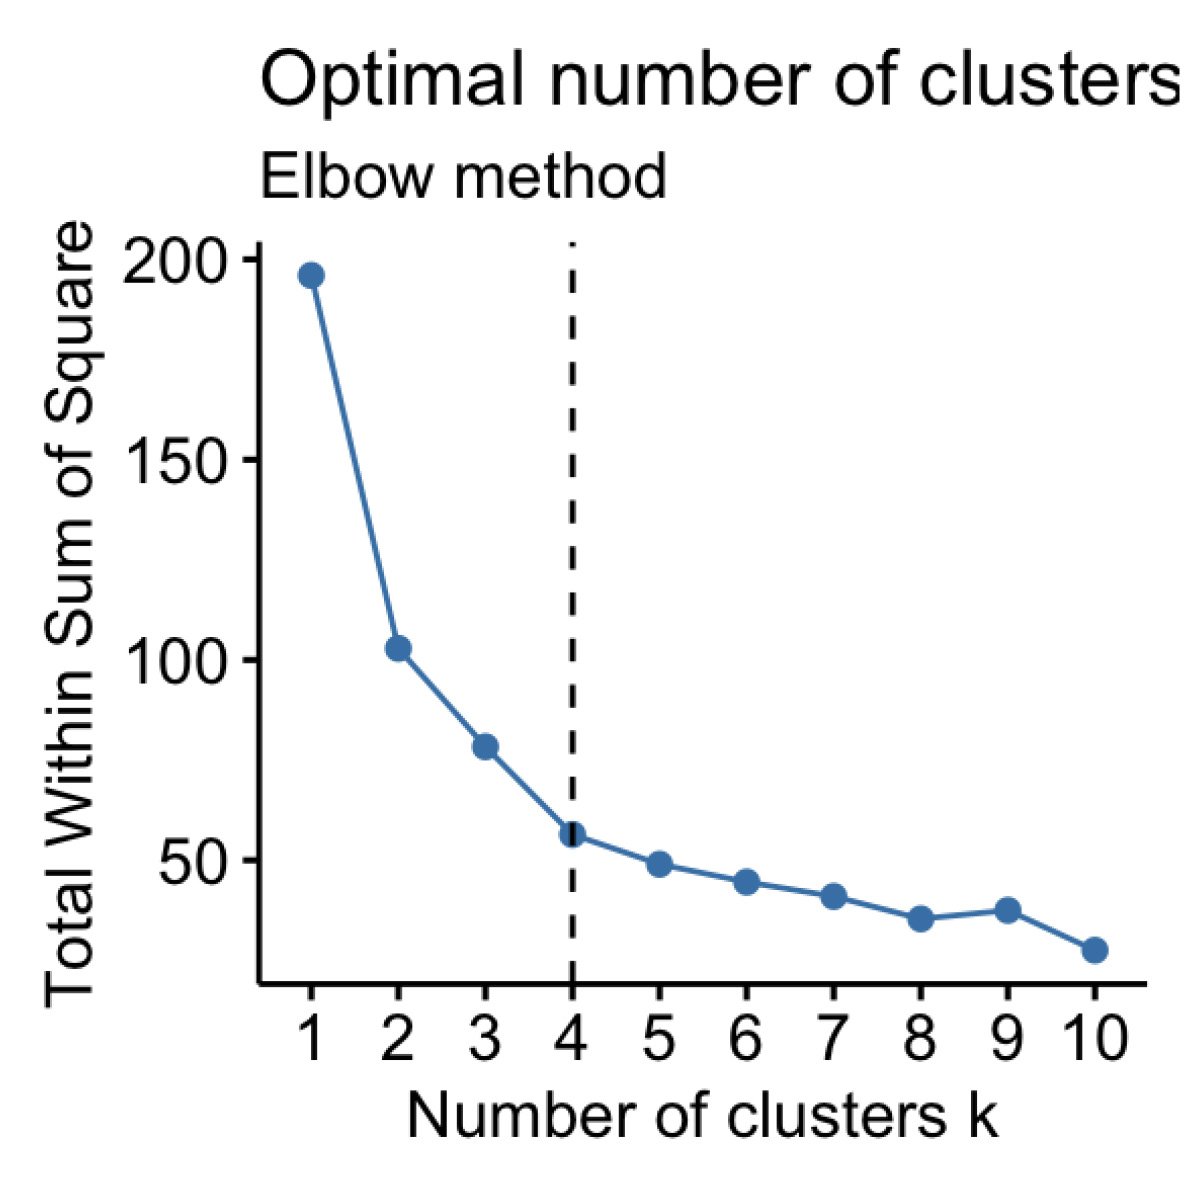
\includegraphics[width=0.4\linewidth]{img/elbow_method_illustration}
	\caption{An example for the elbow method of choosing $K$}
	\label{fig:elbowmethodillustration}
\end{figure}

\subsubsection{Silhouette Method for $K$ Selection}
Given $K$ and $K$ clusters, given any data point $i$, let $a_i$ be the average distance or dissimilarity of $i$ with all other points in the same cluster.
\begin{equation*}
	s_i = \frac{b_i - a_i}{\max(b_i,a_i)} \tag*{\textbf{Silhouette Score} $s_i \in [-1,1]$}
 \end{equation*}
For the Euclidean $k$-means use the Euclidean distance for dissimilarity. $a_i$ measures the fit of $i$ into its cluster and $b_i$ is the smallest average distance of $i$ to other clusters. The score $s_i$ is close to $1$ if point $i$ is in a tight cluster and far away from other clusters. Therefore, $s_i$ is close to $-1$ if $i$ is in a loose cluster and close to other clusters.
\begin{equation*}
	\text{Maximise}\quad \frac{1}{n}\sum_{i=1}^{n}s_i\ \text{over} K
\end{equation*}

\noindent
\begin{minipage}{0.4\linewidth}
	Silhouette analysis can be used to study the separation distance between the resulting clusters.
	\begin{itemize}
		\item[$a_i$:] 5.52
		\item[$b_i$:] 21.82 (because the other cluster is further away by visual inspection)
		\item[$s_i$:] 0.75
	\end{itemize}
	So the $i$th point is in a pretty tight cluster
\end{minipage}
\hfill
\begin{minipage}{0.57\linewidth}
	\includegraphics[width=\linewidth]{img/silhouette_score_example}
\end{minipage}

The silhouette plot displays a measure of how close each point in one cluster is to points in the neighbouring clusters and thus provides a way to assess parameters like number of clusters visually.

The average silhouette method calculates the \textbf{average silhouette of observations} for each $k$. The location of the maximum on the curve of average silhouette as function over the number of clusters $k$ is considered as the appropriate number of clusters.

\begin{center}
	\includegraphics[width=0.9\linewidth]{img/silhouette_plot}
\end{center}

\subsection{Cluster Metrics}

\subsubsection{Inertia $W$}
The \textbf{within-cluster inertia $W$} of the partition $C_K$ is the sum of the \emph{inertia} of the clusters and measures the \textbf{heterogeneity} within the clusters.
\begin{align*}
	W &= \sum_{k=1}^{K} I(C_K)\\
	I(C_K) &= \sum_{i\in C_K} \norm{x_i - \mu_k}^2
\end{align*}
The \textbf{between-cluster inertia $B$} of the partition $C_K$ is the inertia of the gravity centres of the clusters weighted by $\mu_k$ and measures the \emph{separation between the clusters}. A good partition has a \textbf{large between-cluster inertia} and a \textbf{small within-cluster inertia}.

\begin{minted}{python}
Sum_of_squared_distances = []
K = range(1,15) for k in K:
	km = KMeans(n_clusters=k)
	km = km.fit(data_transformed)
	Sum_of_squared_distances.append(km.inertia_)

plt.plot(K, Sum_of_squared_distances, 'bx-')
\end{minted}

\subsubsection{Rand Index Adjusted for Chance (RI and ARI)}
The Rand Index (RI) computes a similarity measure between two clusterings by \emph{considering all pairs of samples and counting pairs that are assigned in the same or different clusters} in the predicted and true clusterings.

Given a set of $n$ elements in $S = \{o_1,\dots,o_n\}$ and two partitions of $S$ to compare, $\textbf{X} = \{X_1,\dots, X_r\}$ a partition of $S$ into $r$ subsets, and $\textbf{Y} = \{Y_1,\dots, Y_s\}$ a partition of $S$ into $s$ subsets, define
\begin{itemize}[nosep]
	\item $a$, the number of pairs of elements in $S$ that are the \textbf{same subset} in $\textbf{X}$ and in the \textbf{same subset} in $\textbf{Y}$
	\item $b$, the number of pairs of elements in $S$ that are \textbf{different subsets} in $\textbf{X}$ and in \textbf{different subsets} in $\textbf{Y}$
	\item $c$, the number of pairs of elements in $S$ that are the \textbf{same subset} in $\textbf{X}$ and in \textbf{different subsets} in $\textbf{Y}$
\end{itemize}
\begin{equation*}
	\text{RI} = \frac{a + b}{a + b + c + d} = \frac{a + b}{\binom{n}{2}} = \frac{\text{TP} + \text{TN}}{\text{TP} + \text{TN} + \text{FP} + \text{FN}}
\end{equation*}
The Rand index RI is ensured to have a value close to $0.0$ for random labelling independent of the number of clusters and samples. It is exactly $1.0$ when the clusterings are identical (up to a permutation).

Since the denominator is the total number of pairs, the Rand index \textbf{RI} represents the \textbf{frequency of occurrence of agreements over the total pairs}, or the probability that $X$ and $Y$ will agree on a randomly chosen pair, or it can be seen as a measure of the percentage of correct decisions made by the algorithm.

The adjusted Rand index ARI is the corrected-for-chance version of the Rand index (permutation model) and is a symmetric model.
\begin{equation*}
	\text{ARI}(X,Y) = \frac{\text{RI} - \ev{\text{RI}}}{\max(\text{RI}) - \ev{\text{RI}}}
\end{equation*}

\subsubsection{Normalised Mutual Information (NMI)}
NMI is a good measure for determining the quality of clustering and an external measure because the class labels of the instances are needed to determine the NMI. As it is normalised, the NMI can be measured and compared between different clusterings having different number of clusters.
\begin{align*}
	\text{NMI} &= \frac{2\cdot I(Y;C)}{H[Y] + H[C]}\\
	I(Y;C) &= H[Y] - \sum_k H[Y|C_k]
\end{align*}
\begin{itemize}[nosep, leftmargin=*, labelindent=5cm, labelsep=0.5cm]
	\item[$I(Y;C)$] mutual information between $Y$ and $C$
	\item[$H\lbrack Y \rbrack$] Entropy of class labels
	\item[$H\lbrack C \rbrack$] Entropy of cluster labels
\end{itemize}
\begin{minted}[breaklines, fontsize=\small]{python}
sklearn.metrics.normalized_mutual_info_score(labels_true, labels_pred, average_method=’warn’)
\end{minted}

\subsubsection{Bayesian Information Criterium (BIC)}
The BIC can measure the efficiency of the parametrised model in terms of predicting the data. It penalises the complexity of the model, here complexity refers to the number of parameters $B = K\cdot d$ used. The BIC can be used to choose the number of clusters according to the intrinsic complexity present in a particular dataset. It is independent of the prior.
\begin{align*}
	\text{BIC} &= \ln{n} \cdot B - 2 \ln{\hat{L}}\\
	&= \ln{n} \cdot (K \cdot d) + W
\end{align*}
\begin{itemize}[nosep, leftmargin=*, labelindent=1.5cm, labelsep=1cm]
	\item[$\hat{L}$] maximised value of the likelihood function of the model $\mathcal{M}$\\
	$\hat{L} = p(x|\hat{\theta},\mathcal{M})$ where $\hat{\theta}$ are the maximum likelihood estimates of the parameters
	\item[$x$] observed data with dimension $d$
	\item[$n$] number of data points
	\item[$B$] number of parameters estimated by the model $\mathcal{M}: B = K\cdot d$
	\item[$W$] within-cluster-inertia $W$ equals to the Residual Sum of Squares
\end{itemize}
\begin{minted}[breaklines, fontsize=\small]{python}
from sklearn import mixture
lowest_bic = np.infty; bic = []
n_components_range = range(1, 7)
for n_components in n_components_range:
	# Fit a Gaussian mixture with EM
	gmm =mixture.GaussianMixture(n_components=n_components, covariance_type='full')
	gmm.fit(X)
	bic.append(gmm.bic(X))
	if bic[-1] < lowest_bic:
		lowest_bic = bic[-1]
		best_gmm = gmm

bic = np.array(bic)
\end{minted}
\begin{figure}[H]
	\centering
	\includegraphics[width=0.8\linewidth]{img/BIC_inertia_plot}
	\caption{An alternative to elbow-curve is the plot of the inertia}
	\label{fig:bicinertiaplot}
\end{figure}

\subsubsection{Density Based Spatial Clustering of Applications with Noise (DBSCAN)}
The basic idea of DBSCAN is that \textbf{clusters form dense regions} in the data and are separated by relatively empty areas. Points within a dense region are called core points. DBSCAN identifies points in densely populated regions of the feature space in which many data points lie close together.

The advantages are that (a) the user \textbf{can't set the number of clusters} beforehand, (b) DBSCAN is able to capture clusters with \textbf{complex shapes} and (c) that it identifies points that do not belong to any of the clusters.

The DBSCAN procedure is slower than the agglomerative clustering and k-Means, but scales relatively well for large data sets.

\begin{itemize}
	\item Two parameters: \texttt{min\_samples} and \texttt{eps}
	\item If at least \texttt{min\_samples} data points are within the distance \texttt{eps} to a given point, this data point is classified as a \textbf{core object}. Core objects that are closer than \texttt{eps} to each other are assigned to the same cluster.
	\item At the start the the algorithm selects any starting point. Then it finds all points at distance \texttt{eps} or closer to this point. If less than \texttt{min\_samples} points are found within the distance \texttt{eps} to the starting point, this point will be classified as \textbf{noise} and not belonging to any cluster.
	\item If there are more than \texttt{min\_samples} points at a distance of \texttt{eps}, the point is used as core object and receives a new cluster designation.
\end{itemize}

\section{Gaussian Mixture Models And The Expectation Maximisation Algorithm}
\subsection{The EM Algorithm: A General-Purpose, Unsupervised Learning Algorithm}
Expectation Maximisation is an iterative method to learn in the presence of unobserved variables. A typical hidden variable is some sort of group or cluster membership. This algorithm has good convergence guarantees.

\begin{enumerate}
	\item Start with a random initial hypothesis
	\item \textbf{E-Step}\\
	Estimate expected values of unobserved variables, assuming the current hypothesis holds
	\item \textbf{M-Step}\\
	Calculate new Maximum Likelihood (ML) estimate of hypothesis, assuming the expected values from (2) hold
	\item Iterate until convergence while always replacing old estimates with new ones
\end{enumerate}

\subsection{K-Means Revisited}
Assume that K is known. The optimisation that leads to the clusters is the following
\begin{flalign*}
	\underset{\textbf{z},\bm{\mu}}{\min}\mathcal{L}(\textbf{z},\bm{\mu}) = \sum_{n=1}^{N}\sum_{k=1}^{K} z_{nk} \norm{\textbf{x}_n - \bm{\mu}_k}^2 &\qquad (\text{K-Means Loss Function})
\end{flalign*}
With $\bm{\mu}_k \in \R^D$, $z_{nk} \in \{0,1\}$, $\sum_{k=1}^{K} z_{nk} = 1$ and where
\begin{alignat*}{2}
\textbf{z}_n &= [z_{n1},z_{n2},\dots,z_{nk}]^T &\qquad& \text{(indicator variable)}\\
\textbf{z} &= [\textbf{z}_1,\textbf{z}_2,\dots,\textbf{z}_N ]^T && \\
\bm{\mu} &= [\bm{\mu}_1,\bm{\mu}_2,\dots,\bm{\mu}_N]^T &&
\end{alignat*}
The indicator variable is an assignment of datapoint $n$ to a certain cluster, also called membership or latent variable (point $n$ belongs to cluster 3, $\textbf{z}_n = [0,0,1,0,\dots,0]^T$).

For fixed centres $\bm{\mu}_k$, the cost is minimised if each sample is mapped to its nearest centre, where the distance is measured in terms of Euclidean distance. In other words, each sample is assigned to \textbf{exactly one centre or cluster}. This is indicated by setting the corresponding indicator variable $z_{nk}$ to 1 and all other ones $z_{nk'}$ to 0. This leads to the very intuitive algorithm
\begin{enumerate}
	\item[(0.)] initialise $\bm{\mu}_k\quad\forall k$
	\item For all $n$, compute $\textbf{z}_n$ given $\bm{\mu}$
	\item For all $k$, compute $\bm{\mu}_k$ given $\textbf{z}$
\end{enumerate}
Calculating the derivative of the cost function with regards to $\bm{\mu}_k$ and solving for the cluster centres yields
\begin{align*}
	\frac{\partial\Likelihood}{\partial\bm{\mu}_k} &= 0\\
	\Rightarrow \bm{\mu}_k = \frac{\sum_{n=1}^{N} z_{nk}\textbf{x}_n}{\sum_{n=1}^{N} z_{nk}}
\end{align*}

\textbf{Convergence} to a \emph{local optimum} is assured since each step decreases the cost (see \cite[Exercise 9.1]{bishop2006pattern}). But note that there is \textbf{no guarantee to reach the globally optimal solution} with this iterative algorithm. K-mean is thus a \textbf{coordinate descent} algorithm
\begin{equation*}
	\underset{\textbf{z},\bm{\mu}}{\min} \Likelihood(\textbf{z},\bm{\mu}) \begin{cases}
	\textbf{z}^{(t+1)} = \argmin{\textbf{z}} \Likelihood(\textbf{z},\bm{\mu}^{(t)})\\
	\bm{\mu}^{(t+1)} = \argmin{\bm{\mu}} \Likelihood(\textbf{z}^{(t)},\bm{\mu})
	\end{cases}
\end{equation*}

\subsection{Probabilistic K-Means}
Assuming that, conditioned that a point is associated to cluster $k$, it is considered a sample for the $D$-dimensional Gaussian with mean $\bm{\mu}_k$ and a covariance matrix $\isocov$, that is the \textbf{likelihood} of a sample $x$ given the cluster assignment $\textbf{z}$ and centres $\bm{\mu}$ is
\begin{equation*}
	p(\textbf{x}|\textbf{z},\bm{\mu}) = \prod_{k=1}^{K}\left[\N{\textbf{x}\middle| \bm{\mu}_k,\isocov}\right]^{z_{nk}}
\end{equation*}
Then, the likelihood for the whole data set is
\begin{equation*}
	p(\textbf{X}|\textbf{z},\bm{\mu}) = \prod_{n=1}^{N}\prod_{k=1}^{K}\left[\N{\textbf{x}\middle| \bm{\mu}_k,\isocov}\right]^{z_{nk}}
\end{equation*}
Calculating the negative logarithm in order to minimise the negative log-likelihood, yields the \textbf{k-means cost function} again
\begin{equation*}
	-\log p(\textbf{X}|\textbf{z},\bm{\mu}) = \sum_{n=1}^{N}\sum_{k=1}^{K}z_{nk}\norm{\textbf{x}_n - \bm{\mu}_k}^2
\end{equation*}

\subsection{Hard and Soft Clustering}
Given a simple data set consisting of class \texttt{heights} $\textbf{X} = \{x_i\}$ with groups $Z = {z_1,z_2}$ separated by gender. Imagine that there are no convenient gender labels associated with each data point. How could the two group means be estimated?

Assume that the observed values $\textbf{X}$ of the \texttt{height} data are drawn from two independent Gaussian distributions with mean $\mu_k$ and variances $\sigma_1^2, \sigma_2^2$. Understanding the range the $z_j$ values can take is important. In \textbf{K-means} the two $z_j$ can only take the values $[0,1]$, which is called \textbf{hard clustering}. In Gaussian Mixture Models, the $z_j$ can take on any value between 0 and 1, which is called \textbf{soft or fuzzy clustering}.

\subsubsection{Clustering with Gaussians}
K-means is equivalent to assuming that the data came from $K$ \emph{spherically symmetric} Gaussians. Instead of isotropic covariances $\isocov$, the full covariance matrices $\bm{\Sigma}_k$ are used to model elliptical clusters.
\begin{equation*}
	p(\textbf{X}|\textbf{z},\bm{\mu},\bm{\Sigma}) = \prod_{n=1}^{N}\prod_{k=1}^{K}\left[\N{\textbf{x}\middle| \bm{\mu}_k,\bm{\Sigma}_k}\right]^{z_{nk}}
\end{equation*}
In K-means each sample belongs to exactly one cluster. This is not always a good choice, especially for points belonging to the boundary. By interpreting $z_n$ as \emph{random variable} taking the values $[1,2,\dots,K]$ with a \emph{prior distribution} that follows a multinomial distribution, define a fractional assignment or \textbf{soft clustering} can be defined.
\begin{align*}
	p(z_n = k) = \pi_k\\
	\pi_k \leq 0\quad k\\
	\sum_{k=1}^{K}\pi_k = 1\\
	p(\textbf{z}) = \prod_{k=1}^{K} (\pi_k)^{z_k}
\end{align*}

\subsection{Gaussian Mixture Models}
A \textbf{Gaussian mixture model} is a probabilistic model that assumes all the data points are generated from a mixture of a finite number $K$ of Gaussian distributions with unknown parameters $(\mu_k, \Sigma_k)$.

One can think of mixture models as generalizing K-means clustering to incorporate information about the covariance structure of the data as well as the centres of the latent Gaussians.
\begin{tabularx}{\linewidth}{m{2cm} X}
	Speed & It is the \textbf{fastest algorithm} for learning mixture models \\
	Agnostic & As this algorithm maximizes only the likelihood, it will not bias the means towards zero, or bias the cluster sizes to have specific structures that might or might not apply. \\
	Singularities & When one has insufficiently many points per mixture, estimating the covariance matrices becomes difficult, and the algorithm is known to diverge and find solutions with infinite likelihood unless one regularizes the covariances artificially.
\end{tabularx}

\begin{figure}[H]
	\begin{subfigure}[t]{0.49\linewidth}
		\includegraphics[width=\linewidth]{img/GMM01}
	\end{subfigure}
	\hfill
	\begin{subfigure}[t]{0.49\linewidth}
		\includegraphics[width=\linewidth]{img/GMM02}
	\end{subfigure}
	\begin{subfigure}[t]{0.49\linewidth}
		\includegraphics[width=\linewidth]{img/GMM03}
	\end{subfigure}
	\hfill
	\begin{subfigure}[t]{0.49\linewidth}
		\includegraphics[width=\linewidth]{img/GMM04}
	\end{subfigure}
\end{figure}

Assume that the samples $\{x_i\}$ are iid samples from a weighted sum of $K$ $D$-dimensional Gaussians. The probability density is characterised by the parameter $\bm{\theta}$
\begin{equation*}
	\bm{\theta} = \{\bm{\mu}, \bm{\Sigma}, \bm{\pi}\}
\end{equation*}
The joint probability density is given by
\begin{align*}
	p(\textbf{X},\textbf{z} | \bm{\mu}, \bm{\Sigma}, \bm{\pi}) &= \prod_{n=1}^{N} p(\textbf{x}_n|z_n,\bm{\mu}, \bm{\Sigma}) \cdot p(z_n|\bm{\pi})\\
	&= \prod_{n=1}^{N}\prod_{k=1}^{K} \left[ \N{\textbf{x}_n\middle|\bm{\mu}_k, \bm{\Sigma}_k} \right]^{z_{nk}} \prod_{k=1}^{K}[\pi_k]^{z_{nk}}
\end{align*}
\textbf{Marginal likelihood}: The $z_n$ are \textbf{latent variables} that can be marginalised out to get a cost function that does not depend on $z_n$.
\begin{equation*}
	p(\textbf{x}_n|\theta) = \sum_{k=1}^{K} \pi_k \N{\textbf{x}_n|\bm{\mu}_k, \bm{\Sigma}_k}
\end{equation*}
\begin{figure}[H]
	\centering
	\includegraphics[width=0.8\linewidth]{img/GMM05}
	\caption{Illustration of a mixture of three Gaussians in a two-dimensional space.\\
	(a) Contours of constant density for each of the mixture components, in which the three components are denoted red, blue and green, and the values of the mixing coefficients are shown below each component. (b) Contours of the marginal probability density $p(\textbf{x})$ of the mixture distribution. (c) A surface plot of the distribution  $p(\textbf{x})$ \parencite{bishop2006pattern}.}
	\label{fig:gmm05}
\end{figure}

\subsubsection{EM Algorithm for GMM}
To determine the unknown parameters the log-likelihood is maximised
\begin{equation*}
	\Likelihood(\theta) = \ln p(\textbf{X}|\bm{\mu}, \bm{\Sigma}, \bm{\pi}) = \sum_{n=1}^{N}\left\{\sum_{k=1}^{K}\pi_k\N{\textbf{x}_n|\bm{\mu}_k, \bm{\Sigma}_k}\right\}
\end{equation*}
Compute the \textbf{cluster assignments} (E-Step)
\begin{equation*}
	\gamma_{nk}^{(t)} = P(z_{nk}|\bm{\theta}^{(t)}, \textbf{x}_n) = \frac{\pi_k^{(t)} \N{\textbf{x}_n|\bm{\mu}_k, \bm{\Sigma}_k}}{\sum_{k=1}^{K}\pi_k^{(t)} \N{\textbf{x}_n|\bm{\mu}_k, \bm{\Sigma}_k}}
\end{equation*}
\textbf{Update the cluster centres, covariances and probabilities} (M-Step)
\begin{align*}
	\bm{\mu}_k^{(t+1)} &= \frac{\sum_{n}\gamma_{nk}^{(t)}\textbf{x}_n}{\sum_{n}\gamma_{nk}^{(t)}}\\
	\pi_k^{(t+1)} &= \frac{1}{N}\sum_n\gamma_{nk}^{(t)}\\
	\bm{\Sigma}_k^{(t+1)} &= \frac{1}{Z^{(t)}} \cdot \sum_n \gamma_{nk}^{(t)} \left(\textbf{x}_n - \bm{\mu}_k^{(t+1)}\right)\left(\textbf{x}_n - \bm{\mu}_k^{(t+1)}\right)^T
\end{align*}
The main difficulty in learning Gaussian mixture models from unlabeled data is that one usually doesn’t know which points came from which \textbf{latent component}.

Expectation-maximisation is a well-founded statistical algorithm to get around this problem by an iterative process.
\begin{itemize}
	\item \textbf{E-Step}\quad First, one assumes random components (randomly centred on data points, learned from k-means, or even just normally distributed around the origin) and computes for each point a probability of being generated by each component of the model.
	\item \textbf{M-Step}\quad Then, one tweaks the parameters to maximise the likelihood of the data given those assignments. Repeating this process is guaranteed to always converge to a local optimum.
\end{itemize}

\subsubsection{GMM Best Practices}
\begin{itemize}
	\item Use log-likelihoods instead of likelihoods\\
	Likelihoods become so small that one ends up with numerical instabilities otherwise
	\item Use a diagonal covariance matrix\\
	Simpler/faster training, same/better results due to more compact model (with more mixtures)
	\item Use a variance limit and beware of curse of dimensionality\\
	Prohibit artifacts through underestimation of components
	\item Find optimal number of mixtures for data via brute force and BIC
	\item Compare models via
	\begin{itemize}
		\item Score-wise (more precise): Generalized Likelihood Ratio (GLR)
		\item Parameter-wise (faster): Earth Mover‘s Distance (EMD) \parencite{beigi1998distance}
	\end{itemize}
\end{itemize}

%% APPENDIX %%

\printbibliography

\end{document}
